


\newpage


\section{Exploration of an Interdisciplinary Scientific Landscape}{Exploration d'un paysage scientifique interdisciplinaire}

\label{app:sec:cybergeo}


%----------------------------------------------------------------------------------------



Les constructions méthodologiques et techniques rendant possible l'analyse épistémologique de~\ref{sec:quantepistemo} ont été menées dans un cadre plus large, notamment débutant avec l'analyse de corpus construits à partir de la revue \textit{Cybergeo}. Nous détaillons ici l'aspect méthodologique des ces analyses.

 
\stars

\textit{Le contenu de cette annexe a été élaboré dans le cadre du projet commun d'analyse quantitative des publications de Cybergeo (voir \ref{app:sec:cybergeonetworks} pour la production commune), initié pour les 20 ans de la revue en mai 2016. Les résultats préliminaires ont été présentés comme~\cite{raimbault2016indirect} à la conférence anniversaire, et le texte de cette annexe est extrait et traduit de~\cite{raimbault2017exploration}.}


\stars



%----------------------------------------------------------------------------------------


\bpar{
Patterns of interdisciplinarity in science can be quantified through diverse complementary dimensions. This paper studies as a case study the scientific environment of a generalist journal in Geography, \emph{Cybergeo}, in order to introduce a novel methodology combining citation network analysis and semantic analysis. We collect a large corpus of around 200,000 articles with their abstracts and the corresponding citation network that provides a first citation classification. Relevant keywords are extracted for each article through text-mining, allowing us to construct a semantic classification. We study the qualitative patterns of relations between endogenous disciplines within each classification, and finally show the complementarity of classifications and of their associated interdisciplinarity measures. The tools we develop accordingly are open and reusable for similar large scale studies of scientific environments.
}{
Les motifs d'interdisciplinarité en science peuvent être quantifiés au travers de diverses dimensions complémentaires. Cette monographie étudie comme cas d'étude l'environnement scientifique d'un journal généraliste en géographie, \emph{Cybergeo}, afin d'introduire une nouvelle méthodologie qui combine analyse du réseau de citation et analyse sémantique. Nous construisons un corpus massif d'environ 200,000 articles avec leur résumés et le réseau de citation correspondant qui fournit une première classification par citations. Les mots-clés pertinents sont extraits pour chaque article par analyse textuelle, permettant la construction d'une classification sémantique. Nous étudions les motifs qualitatifs de relations entre disciplines endogènes au sein de chaque classification, et montrons finalement la complémentarité des classifications et des mesures d'interdisciplinarité associées. Les outils développés en conséquence sont ouverts et réutilisables pour des études similaires à grande échelle d'environnements scientifiques.
}


%%%%%%%%%%%%%%%%%%%%%%%
\subsection{Introduction}{Introduction}
%%%%%%%%%%%%%%%%%%%%%%%



\bpar{
We develop in this paper a case study coupling citation network exploration and analysis with text-mining, aiming at mapping the scientific landscape in the neighborhood of a particular journal. We choose to study an electronic journal in Geography, named \textit{Cybergeo}\footnote{\texttt{http://cybergeo.revues.org/}}, that publishes articles within all subfields of Geography and is in that way multidisciplinary. The choice is initially due to data availability, but ensures several constraints making it highly relevant to the context given above. First of all, the ``discipline'' of Geography is very broad and by essence interdisciplinary~\cite{bracken2016interdisciplinarity} : the spectrum ranges from Human and Critical geography to physical geography and geomorphology, and interactions between these subfields are numerous. Secondly, bibliographical data is difficult to obtain, raising the concern of how the perception of a scientific landscape may be shaped by actors of the dissemination and thus far from objective, and making technical solutions as the ones we will consequently develop here crucial tools for an open and neutral science. Finally it makes a particularly interesting case study as the editorial policy is generalist and concerned with open science issues such as peer-review ethics transparency~\citep{10.1371/journal.pone.0147913}, open data and model practices, as recalled by~\cite{pumain2015adapting}, and this work contributes to these by fostering the opening of reflexivity.
}{
Cette section développe un cas d'étude qui couple exploration et analyse du réseau de citation avec analyse textuelle, dans le but de cartographier le paysage scientifique du voisinage d'un journal particulier. Nous choisissons d'étudier un journal électronique en Géographie, appelé \textit{Cybergeo}\footnote{\texttt{http://cybergeo.revues.org/}}, qui publie des articles dans l'ensemble des champs de la Géographie et est de cette façon multi-disciplinaire. Le choix est initialement dû à la disponibilité des données, mais répond à différentes contraintes le rendant particulièrement pertinent dans le contexte décrit précédemment. Tout d'abord, la ``discipline'' de la Géographie est très large et par essence interdisciplinaire~\cite{bracken2016interdisciplinarity}: le spectre s'étend de la Géographie Humaine et Critique à la Géographie Physique et la géomorphologie, et les interactions entre ces sous-champs sont nombreuses. Dans un second temps, les données bibliographiques sont difficiles à obtenir, soulevant la difficulté de la façon dont un paysage scientifique est perçu peut être influencée par les acteurs de la dissémination et donc loin d'être objectif, ce qui rend ainsi des solutions techniques comme celle que nous développerons en conséquence ici des outils cruciaux pour une science ouverte et neutre. Enfin, il s'agit d'un cas d'étude particulièrement intéressant puisque la politique éditoriale est généraliste et préoccupée par des questions de science ouverte comme la transparence de l'éthique de revue par les pairs~\cite{10.1371/journal.pone.0147913}, les pratiques d'ouverture des données et des modèles, comme rappelé par~\cite{pumain2015adapting}, et ce travail contribue à celles-ci en encourageant l'ouverture de la reflexivité.
}


% idem main text
%\bpar{
%Our approach combine semantic communities analysis with citation network analysis to extract features such as interdisciplinarity measures. Our contribution differs from the previous works quantifying interdisciplinarity as it does not assume predefined domains nor classification of the considered papers, but reconstructs from the bottom-up the fields with the endogenous semantic information. \cite{nichols2014topic} already introduced a close approach, using Latent Dirichlet Allocation topic modeling to characterize interdisciplinarity of awards in particular sciences. \cite{palchykov2016ground} takes a similar approach for papers in physics based on concept extraction from full texts, and show that the endogenous classes differ from the top-down subjects classification. Semantic networks are otherwise well studied in social sciences, such as for example \cite{2015arXiv151003797G} that analyze semantic networks of political debates.
%}{
%Notre approche combine l'analyse de communautés sémantiques avec l'analyse de réseau de citation pour extraire des caractéristiques comme des mesures d'interdisciplinarité. Notre contribution diffère des précédent travaux quantifiant l'interdisciplinarité car elle ne suppose pas de domaines prédéfinis ou de classification des articles considérés, mais reconstruit par le bas les champs avec l'information sémantique endogène. \cite{nichols2014topic} a déjà introduit une approche analogue, en utilisant la modélisation de thématiques par \emph{Latent Dirichlet Allocation} pour caractériser l'interdisciplinarité de prix dans des disciplines particulières. \cite{palchykov2016ground} prend une approche similaire pour des articles en physique en se basant sur l'extraction de concepts à partir des textes complets, et montre que les classes endogènes diffèrent de la classification des sujets par le haut. Les réseaux sémantiques sont par ailleurs largement étudiés en sciences sociales, comme par exemple \cite{2015arXiv151003797G} qui analyse les réseaux sémantiques de débats politiques.
%}


\bpar{
Our contribution is original and significant on at least two aspects :
\begin{enumerate}
	\item we combine endogenous classifications in a network multilayer fashion, using semantic information ;
	\item a large dataset is constructed from scratch to study a journal not referenced in main databases, tackling both data retrieval and large scale data processing issues.
\end{enumerate}
}{
Le contexte méthodologique dans lequel ce travail se situe est développé en~\ref{sec:quantepistemo}. Cette contribution est originale et significative sur au moins deux aspects :
\begin{enumerate}
	\item nous combinons des classifications endogènes dans l'idée d'un réseau multi-couches, en utilisant l'information sémantique ;
	\item un jeux de données massif est construit à partir de rien pour étudier un journal non référencé dans les bases principales, répondant ainsi à des problèmes à la fois liés à la collecte de données et au traitement de données massives.
\end{enumerate}
}


\bpar{
The rest of the paper is organized as follows : we describe in the next section the dataset used and the data collection procedure. We then study properties of the citation network and describe the procedure to construct the semantic classification through text-mining. We finally study complementary measures of interdisciplinarity obtained with the different classifications.
}{
Le reste de cette section est organisée de la façon suivante : nous décrivons d'abord le jeu de données utilisé et la procédure de collecte des données. Nous étudions ensuite les propriétés du réseau de citation et décrivons la procédure pour construire la classification sémantique par analyse textuelle. Nous étudions finalement des mesures complémentaires d'interdisciplinarité obtenues par les différentes classifications.
}



%%%%%%%%%%%%%%%%%%%%%%%
\subsection{Database Construction}{Construction de la base de données}
%%%%%%%%%%%%%%%%%%%%%%%



\bpar{
Our approach imposes some requirements on the dataset used, namely: (i) cover a certain neighborhood of the studied journal in the citation network in order to have a consistent view on the scientific landscape; (ii) have at least a textual description for each node. For these to be met, we need to gather and compile data from heterogeneous sources. We use therefore an application specifically designed, which general architecture is given in Fig.~\ref{fig:cybergeo:fig1}. Source code of the application and all scripts used in this paper are available on the open \texttt{git} repository of the project\footnote{at \texttt{https://github.com/JusteRaimbault/HyperNetwork}}. Raw and processed data are also openly available on Dataverse\footnote{at \texttt{http://dx.doi.org/10.7910/DVN/VU2XKT}}. We recall that an important contribution of this paper is the construction of such an hybrid dataset from heterogeneous sources, and the development of associated tools that can be reused and further developed for similar purposes.
}{
Notre approche impose des contraintes sur le jeu de données utilisé, à savoir : (i) couvrir un certain voisinage du journal étudié dans le réseau de citation pour avoir une vue cohérente sur le paysage scientifique ; (ii) avoir au moins une description textuelle pour chaque noeud. Pour satisfaire celles-ci, nous devons rassembler et compiler des données de sources hétérogènes. Nous utilisons pour cela une application spécifiquement conçue, dont l'architecture générale est donnée en Fig.~\ref{fig:cybergeo:fig1}. Le code source de l'application et l'ensemble des scripts utilisés ici sont disponibles sur le dépôt \texttt{git} ouvert du projet\footnote{à \texttt{https://github.com/JusteRaimbault/HyperNetwork}}. Les données brutes et traitées sont également disponibles de manière ouverte sur Dataverse\footnote{à \texttt{http://dx.doi.org/10.7910/DVN/VU2XKT}}. Nous rappelons qu'une importante contribution de ce travail est la construction d'un tel jeu de données hybride à partir de sources hétérogènes, et le développement d'outils associés qui peuvent être utilisés et étendus dans des cadres similaires.
}


%%%%%%%%%%%%%%%%%%
\begin{figure}
%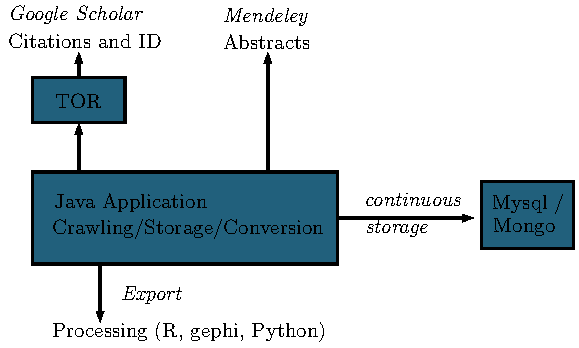
\includegraphics[width=\textwidth]{Figures/Cybergeo/Fig1.pdf}
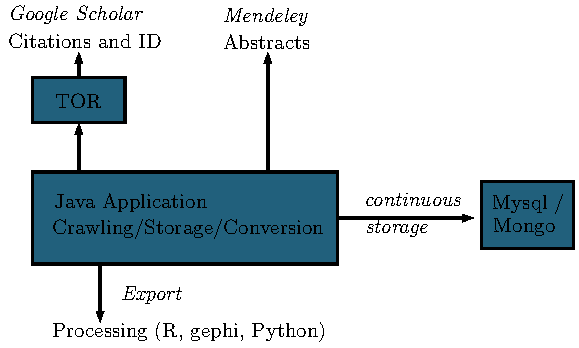
\includegraphics[width=\linewidth]{Figures/Final/B-cybergeo-fig1.pdf}
\appcaption{\textbf{Heterogeneous Bibliographical Data Collection and processing.} Architecture of the application for content (semantic data), metadata and citation data collection. The heterogeneity of tasks requires the use of multiple languages : data collection and management is done in Java, and data stored in databases (Mysql and MongoDB) ; data processing is done in python for Natural Language Processing and in R for statistical and network analyses; graph visualizations are done with Gephi software.\label{fig:cybergeo:fig1}}{\textbf{Collecte et traitement de données bibliographiques hétérogènes.} Architecture de l'application pour la récolte des données de contenu (données sémantiques), des métadonnées et des données de citation. L'hétérogénéité des tâches requière l'utilisation de multiples langages : la collecte et la gestion des données sont faites en Java, et les données sont stockées dans des bases de données (Mysql et MongoDB) ; le traitement des données est effectué en python pour le traitement du langage naturel et en R pour les analyses statistiques et de réseaux ; les visualisations de graphes sont effectuées avec le logiciel Gephi.\label{fig:cybergeo:fig1}}
\end{figure}
%%%%%%%%%%%%%%%%%%




%%%%%%%%%%%%%%%%%%
\subsubsection{Initial Corpus}{Corpus initial}

\bpar{
The production database of \textit{Cybergeo} (snapshot taken in February 2016, provided by the editorial board), provides after pre-processing the initial database of articles, with basic information (title, abstract, publication year, authors). The processed version used is available together with the full database constructed, as a \texttt{mysql} dump, at the address given above. This base provide also bibliographical records of articles that give all references cited by the initial base (\emph{forward citations} for the initial corpus).
}{
La base de production de \textit{Cybergeo} (snapshot pris en février 2016, fournit par l'équipe éditoriale), permet d'obtenir après pré-traitement la base initiale des articles, avec information élémentaire (titre, résumé, année de publication, auteurs). La version traitée que l'on utilise est disponible en même temps que l'ensemble des données construites, comme dump \texttt{mysql}, à l'adresse donnée précédemment. Cette base fournit également les enregistrements de la bibliographie des articles, qui fournissent l'ensemble des références citées par la base initiale (citations \emph{données} par le corpus initial).
}


%%%%%%%%%%%%%%%%%%
\subsubsection{Citation Data}{Données de citation}


\bpar{
Citation data is collected from \texttt{Google Scholar}, that is the only source for incoming citations~\citep{noruzi2005google} in our case as the journal is poorly referenced in other databases\footnote{or was just added as in the case of \textit{Web of Science}, indexing \textit{Cybergeo} since May 2016 only}. We are aware of the possible biaises using this single source (see e.g.~\cite{bohannon2014scientific})\footnote{or \texttt{http://iscpif.fr/blog/2016/02/the-strange-arithmetic-of-google-scholars}}, but these critics are more directed towards search results or possible targeted manipulations than the global structure of the citation network. The automatic collection requires the use of a crawling software to pipe requests, namely \texttt{TorPool}~\citep{torpool} that provides a Java API allowing an easy integration into our application of data collection. A crawler can therethrough retrieve html pages and get backward citation data, i.e. all citing articles for a given initial article. We retrieve that way two sub-corpuses: references citing papers in \textit{Cybergeo} and references \emph{citing the ones cited} by \textit{Cybergeo}. At this stage, the full corpus contains around $4\cdot10^5$ references.
}{
Les données de citation sont collectées à partir de \texttt{Google Scholar}, qui est la seule source pour les citations entrantes~\cite{noruzi2005google} dans notre cas puisque le journal n'est pas référencé dans les autres bases\footnote{ou vient d'y être ajouté comme dans le cas du \emph{Web of Science} qui n'indexe \textit{Cybergeo} que seulement depuis mai 2016}. Nous sommes conscient des possibles biais de l'utilisation de cette source unique (voir par exemple~\cite{bohannon2014scientific})\footnote{ou \texttt{http://iscpif.fr/blog/2016/02/the-strange-arithmetic-of-google-scholars}}, mais ces critiques sont plutôt dirigées vers les résultats de recherche ou de possibles manipulations ciblées que envers la structure globale du réseau de citation. La collecte automatique demande l'utilisation d'un logiciel de collecte pour transférer les requêtes, à savoir \texttt{TorPool}~\cite{torpool} qui fournit une API Java permettant une intégration aisée au sein de notre application de collecte. Un crawler peut ainsi récupérer les pages html et obtenir les citations inverses, c'est-à-dire l'ensemble des articles citant un article initial donné. Nous récupérons de cette manière deux sous-corpus : les références citant des articles dans \textit{Cybergeo} et les références citant celles citées par \textit{Cybergeo}. A ce stade, le corpus complet contient autour de $4\cdot10^5$ références.
}

\bpar{
For the sake of simplicity, we will denote by \emph{reference} any standard scientific production that can be cited by another (journal paper, book, book chapter, conference paper, communication, etc.) and contains basic records (title, abstract, authors, publication year). We work in the following on networks of references, linked by citations.
}{
Pour simplifier, nous appellerons \emph{référence} toute production scientifique standard qui peut être citée par une autre (article de journal, livre, chapitre de livre, article de conférence, communication, etc.) et contient des champs basiques (titre, résumé, auteurs, année de publication). Nous travaillons par la suite sur le réseau de références, reliées par des citations.
}


%%%%%%%%%%%%%%%%%%
\subsubsection{Text Data}{Données textuelles}


\bpar{
A textual description for all references is necessary for a complete semantic analysis. We use for this an other source of data, that is the online catalog of \textit{Mendeley} reference manager software~\cite{mendeley}. It provides a free API allowing to get various records under a structured format. Although not complete, the catalog provides a reasonable coverage in our case, around 55\% of the full citation network. This yields a final corpus with full abstracts of size $2.1\cdot 10^5$. The structure and descriptive statistics of the corresponding citation network is recalled in Fig.~\ref{fig:cybergeo:fig2}.
}{
Une description textuelle pour l'ensemble des références est nécessaire pour une analyse sémantique complète. Nous utilisons pour cela une autre source de données, qui est le catalogue en ligne du logiciel de gestion bibliographique \textit{Mendeley}~\cite{mendeley}. Celui fournit une API gratuite permettant de récupérer divers champs sous un format structuré. Même s'il n'est pas complet, le catalogue fournit une couverture raisonnable dans notre cas, autour de 55\% du réseau de citation complet. Cela correspond à un corpus final avec résumés complets de taille $2.1\cdot 10^5$. La structure et les statistiques descriptives du réseau de citation correspondant sont rappelés en Fig.~\ref{fig:cybergeo:fig2}.
}

%\cite{moreno2016uncertainty} no pb of uncertainty : endogenous classification



%%%%%%%%%%%%%%%%%%
\begin{figure}
%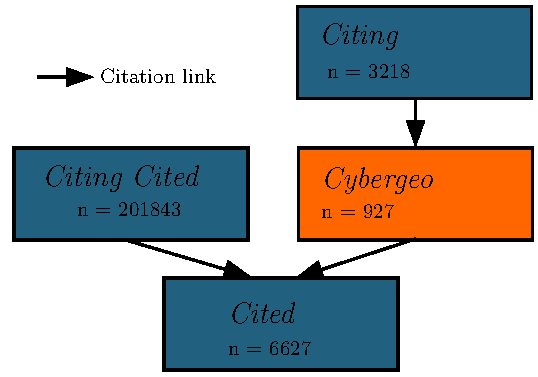
\includegraphics[width=0.6\textwidth]{Figures/Cybergeo/Fig2.pdf}
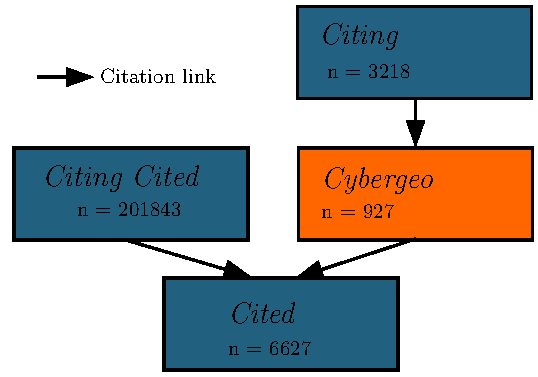
\includegraphics[width=\linewidth]{Figures/Final/B-cybergeo-fig2.pdf}
\appcaption{\textbf{Structure and content of the citation network.} The original corpus of \emph{Cybergeo} is composed by 927 articles, themselves cited by a slightly larger corpus (yielding a stationary impact factor of around 3.18), cite $\simeq 6600$ references, themselves co-cited by more than $2\cdot 10^5$ works for which we have a textual description.\label{fig:cybergeo:fig2}}{\textbf{Structure et contenu du réseau de citation.} Le corpus initial de \emph{Cybergeo} est composé de 927 articles, eux-mêmes cités par un corpus légèrement plus grand (donnant un facteur d'impact stationnaire autour de 3.18), cite $\simeq 6600$ références, elles-mêmes co-citées par plus de $2\cdot 10^5$ travaux pour lesquels nous avons une description textuelle.\label{fig:cybergeo:fig2}}
\end{figure}
%%%%%%%%%%%%%%%%%%









%%%%%%%%%%%%%%%%%%
\subsection{Methods and Results}{Méthodes et Résultats}
%%%%%%%%%%%%%%%%%%



%%%%%%%%%%%%%%%%%%
\subsubsection{Citation Network Properties}{Propriétés du réseau de citation}

\paragraph{Properties}{Propriétés}

% mean(degree(gcitation,which(degree(gcitation,mode="in")>0),mode="in"))
%[1] 121.5615

\bpar{
As detailed above, we are able by the reconstruction of the citation network at depth $\pm 1$ from the original $927$ references of the journal to retrieve around $4\cdot 10^5$ references, on which $2.1\cdot 10^5$ have an abstract text allowing semantic analysis. A first glance on citation network properties provides useful insights. Mean in-degree (that can be interpreted as a stationary integrated impact factor) on references for which it can be defined has a value of $\bar{d}=121.6$, whereas for articles in \textit{Cybergeo} we have $\bar{d}=3.18$. This difference suggests a variety for status of references, from old classical works (the most cited has 1051 incoming citations) to recent less influential works.
}{
Comme détaillé précédemment , nous sommes en mesure de récupérer autour de $4\cdot 10^5$ références par reconstruction du réseau de citation à profondeur $\pm 1$ à partir des $927$ références initiales du journal, parmi lesquelles $2.1\cdot 10^5$ ont un texte de résumé permettant une analyse sémantique. Un premier regard sur les propriétés du réseau de citation fournit des informations utiles. Le degré moyen entrant (qui peut être interprété comme un facteur d'impact stationnaire intégré) pour les références pour lesquelles il peut être défini a une valeur de $\bar{d}=121.6$, tandis que pour les articles de \textit{Cybergeo} nous avons $\bar{d}=3.18$. Cette différence suggère une variété de status de références, de travaux anciens classiques (le plus cité a 1051 citations entrantes) à des travaux plus récents moins influents.
}

%%%%%%%%%%%%%%%%%
\begin{figure}
%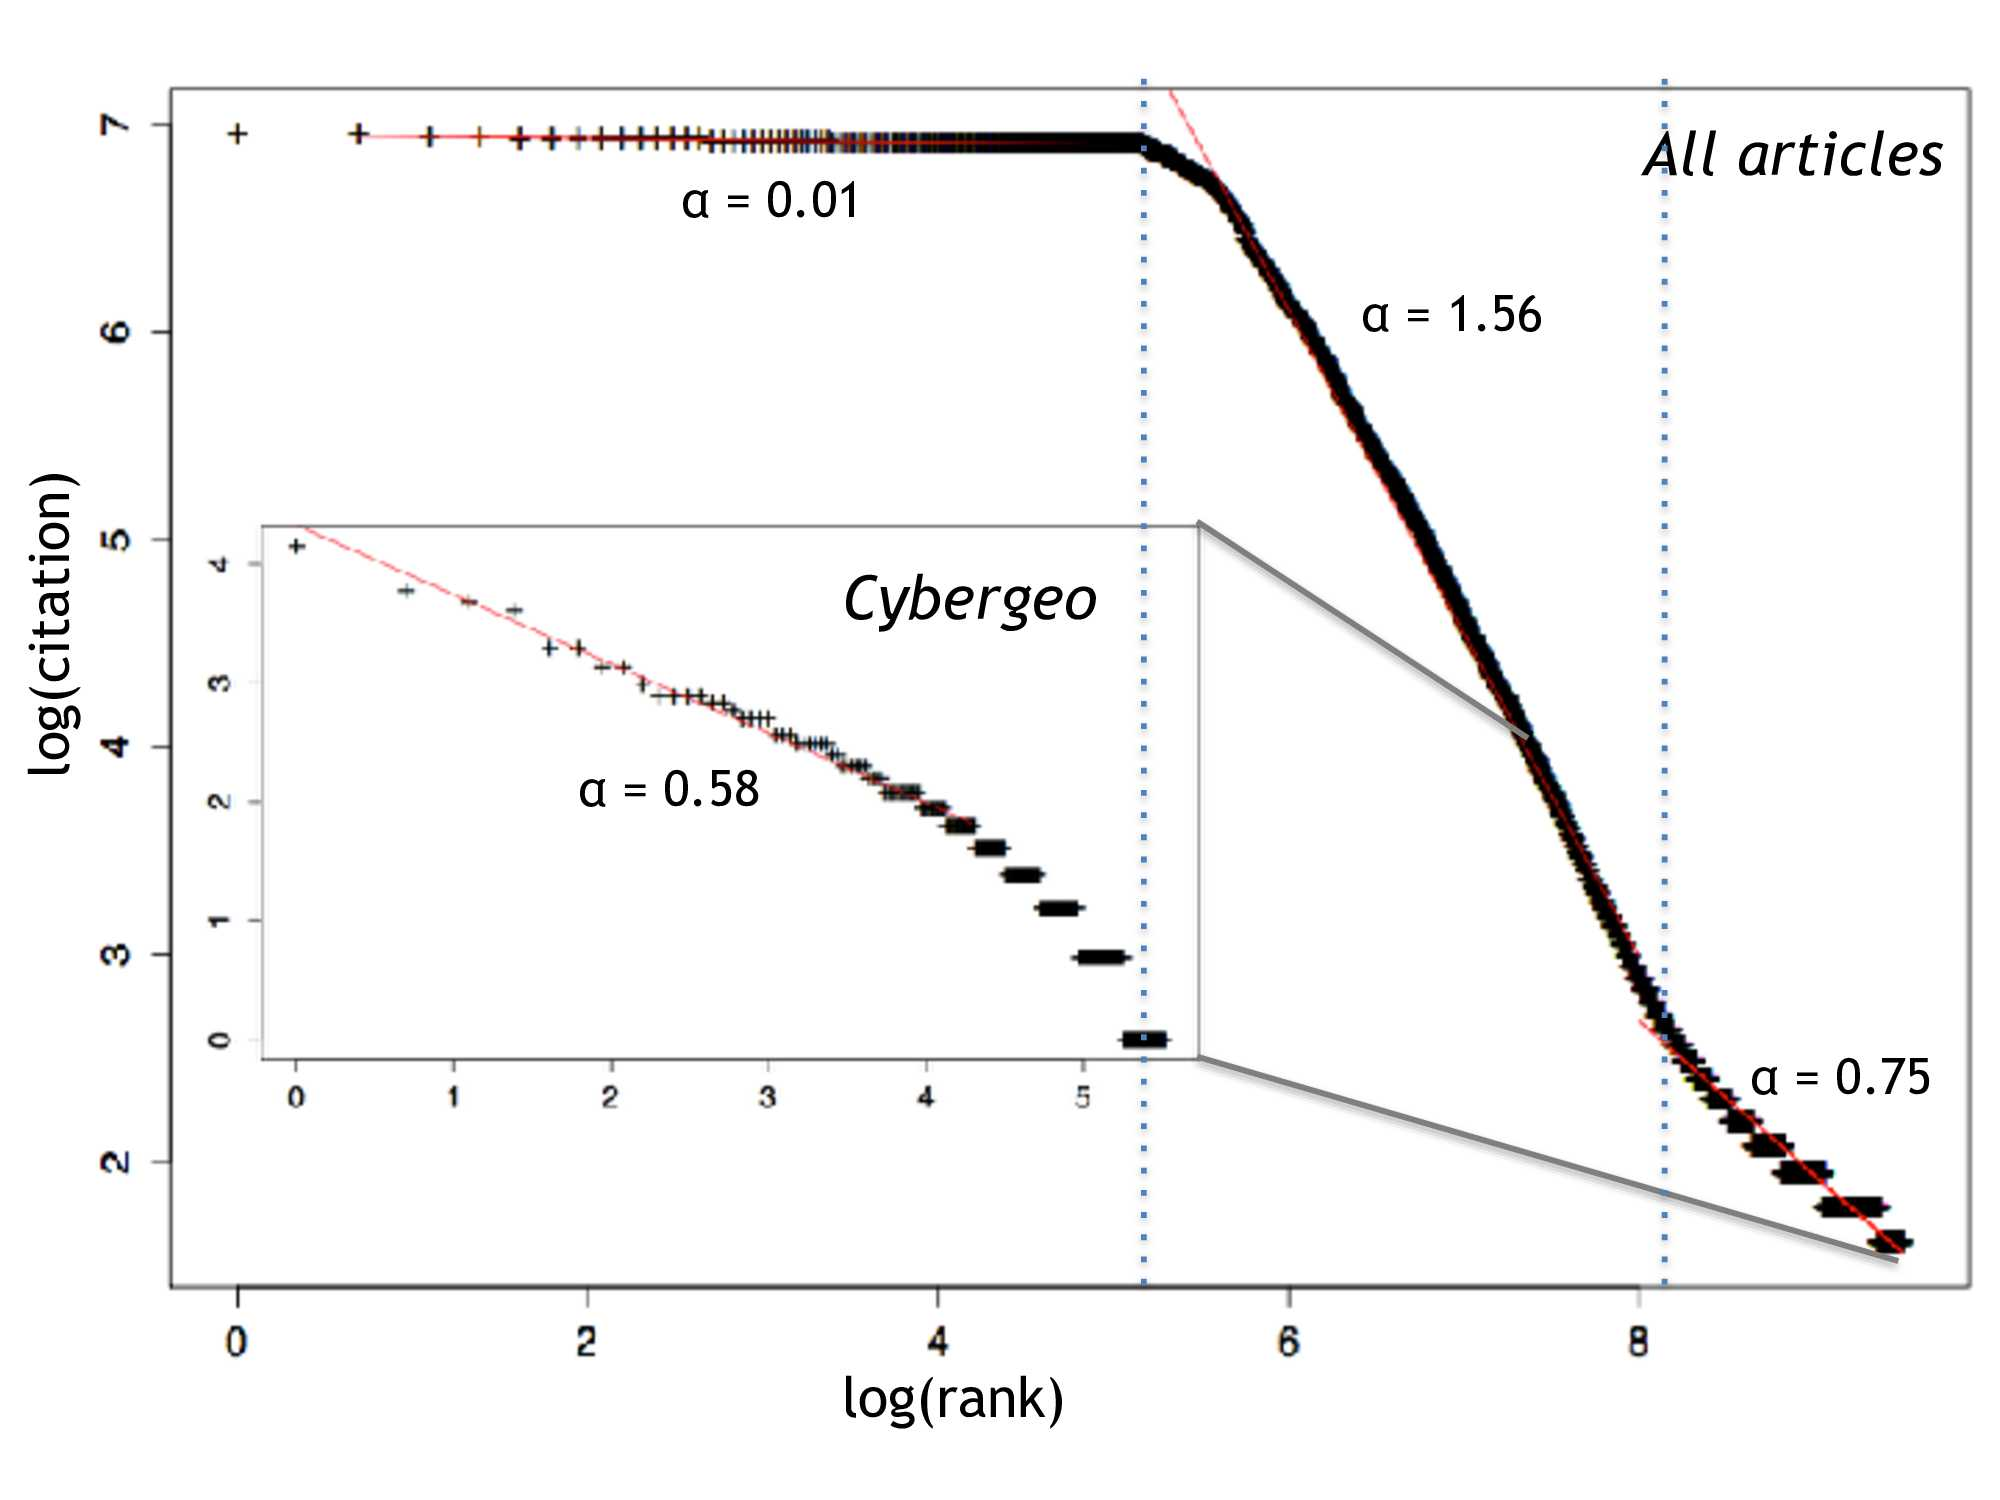
\includegraphics[width=\textwidth]{Figures/Cybergeo/Fig3.jpg}
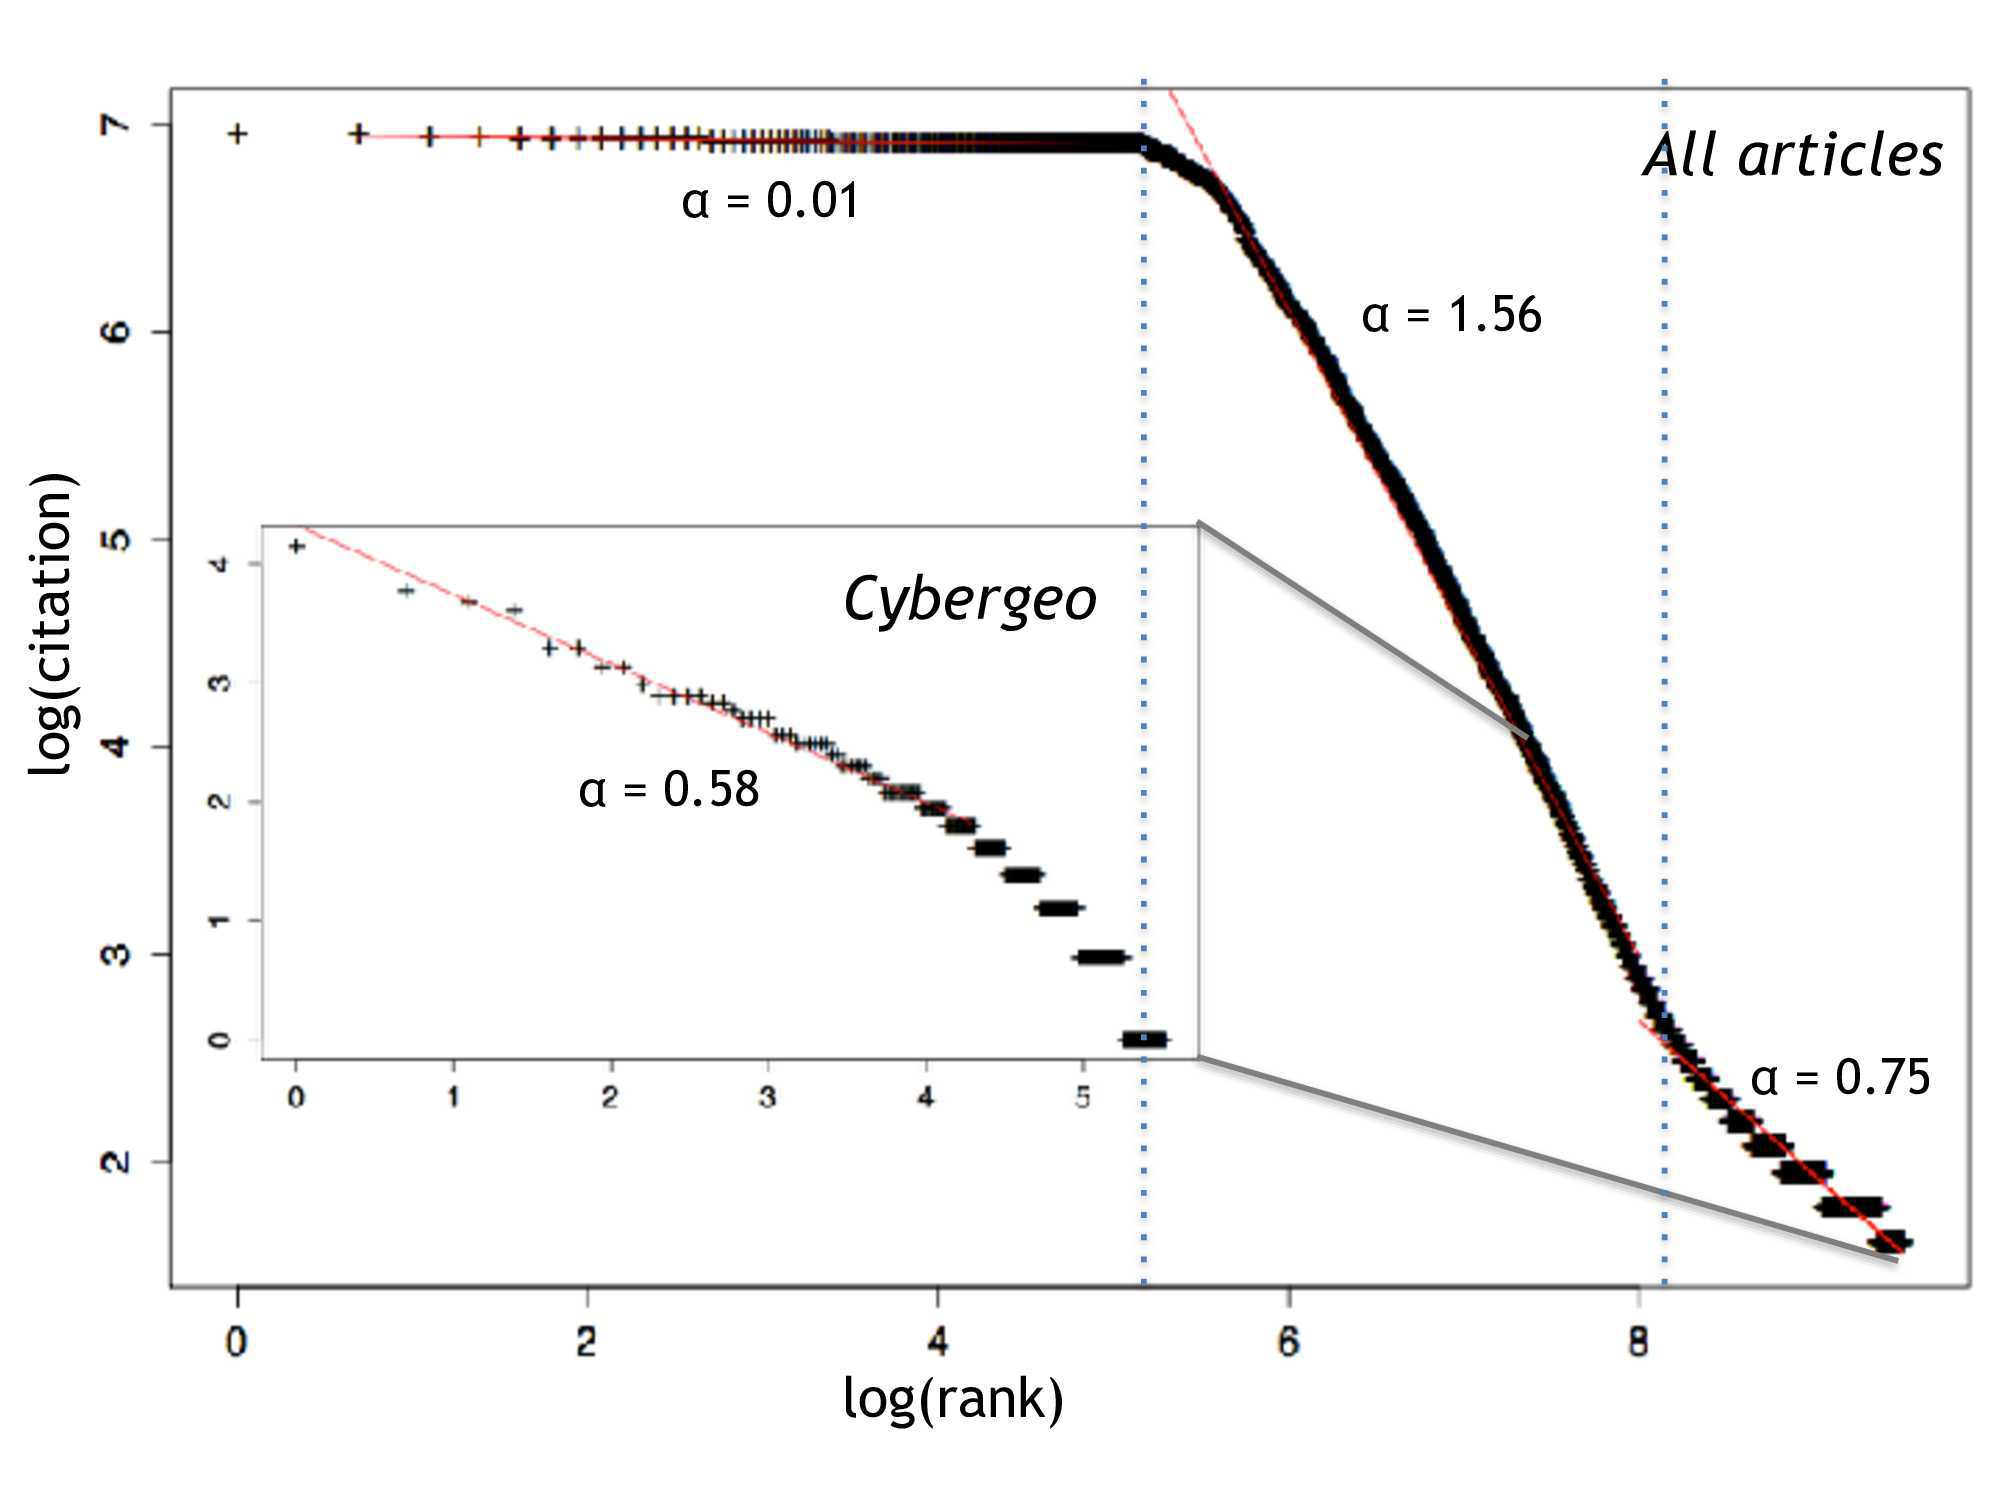
\includegraphics[width=\linewidth]{Figures/Final/B-cybergeo-fig3.jpg}
\appcaption{\textbf{Rank-size plot of citations received.} The plot unveils three superposed citations regimes, corresponding to power laws with different levels of hierarchy. The references in \textit{Cybergeo} (inset plot) are themselves in the tail and less hierarchical.\label{fig:cybergeo:fig3}}{\textbf{Graphe rang-taille des citations reçues.} La courbe dévoile trois régimes de citation superposés, correspondant à des loin puissance avec différents niveaux de hiérarchie. Les références dans \textit{Cybergeo} (graphe en insert) sont elles-mêmes dans la queue et moins hiérarchiques.\label{fig:cybergeo:fig3}}
\end{figure}
%%%%%%%%%%%%%%%%%


\bpar{
This diversity is confirmed by the hierarchical organisation examined in Fig.~\ref{fig:cybergeo:fig3} that unveils three superposed regimes. More precisely, we look at the rank-size plot, given by the logarithm of the number of citations received as a function of the rank of the paper. We find, as expected~\citep{redner1998popular}, localized power-law behaviors. A first set of around 150 references shows a very low hierarchy (rank-size exponent $\alpha = 0.01$) and corresponds to classical references in different disciplines. A second regime ($\alpha = 1.56$) is much more hierarchized, followed by a last regime less hierarchical ($\alpha = 0.75$) containing more recent papers (average publication year mid-2005, against mid-1998 for the second and 1983 for the first).
}{
Cette diversité est confirmée par l'organisation hiérarchique examinée en Fig.~\ref{fig:cybergeo:fig3} qui révèle trois régimes superposés. Plus précisément, nous nous intéressons à la courbe rang-taille, donnée par le logarithme du nombre de citations reçues comme fonction du logarithme du rang de l'article. Nous obtenons, comme attendu \cite{redner1998popular}, des comportements de loi puissance localisés. Un premier ensemble d'environ 150 références présente une hiérarchie très faible (exposant rang-taille $\alpha = 0.01$) et correspond aux références classiques dans différentes disciplines. Un second régime ($\alpha = 1.56$) est bien plus hiérarchisé, suivi par un dernier régime moins hiérarchique ($\alpha = 0.75$) contenant des articles plus récents (année moyenne de publication mi-2005, contre mi-1998 pour le second et 1983 pour le premier).
}


\bpar{
Other topological properties reveal typical patterns of citation practices: for example, the existence of high-order cliques (complete sub-networks) implies citation practices which compatibility with the cumulative nature of knowledge may be questionable~\cite{pumain2005cumulativite}, since these need always to source back the production of knowledge in the most recent works. An exemple of such a clique in shown in Fig.~\ref{fig:cybergeo:fig4}.
}{
D'autres propriétés topologiques révèlent des motifs typiques de pratiques de citation : par exemple, l'existence de cliques (sous-graphes complets) de fort ordre implique des pratiques de citation dont la compatibilité avec la nature cumulative de la connaissance peut être remise en question~\cite{pumain2005cumulativite}, puisque celles-ci doivent toujours trouver la source de la production de connaissance dans les travaux les plus récents. Un exemple de telle clique est montré en Fig.~\ref{fig:cybergeo:fig4}.
}


%%%%%%%%%%%%%%%%%
\begin{figure}
%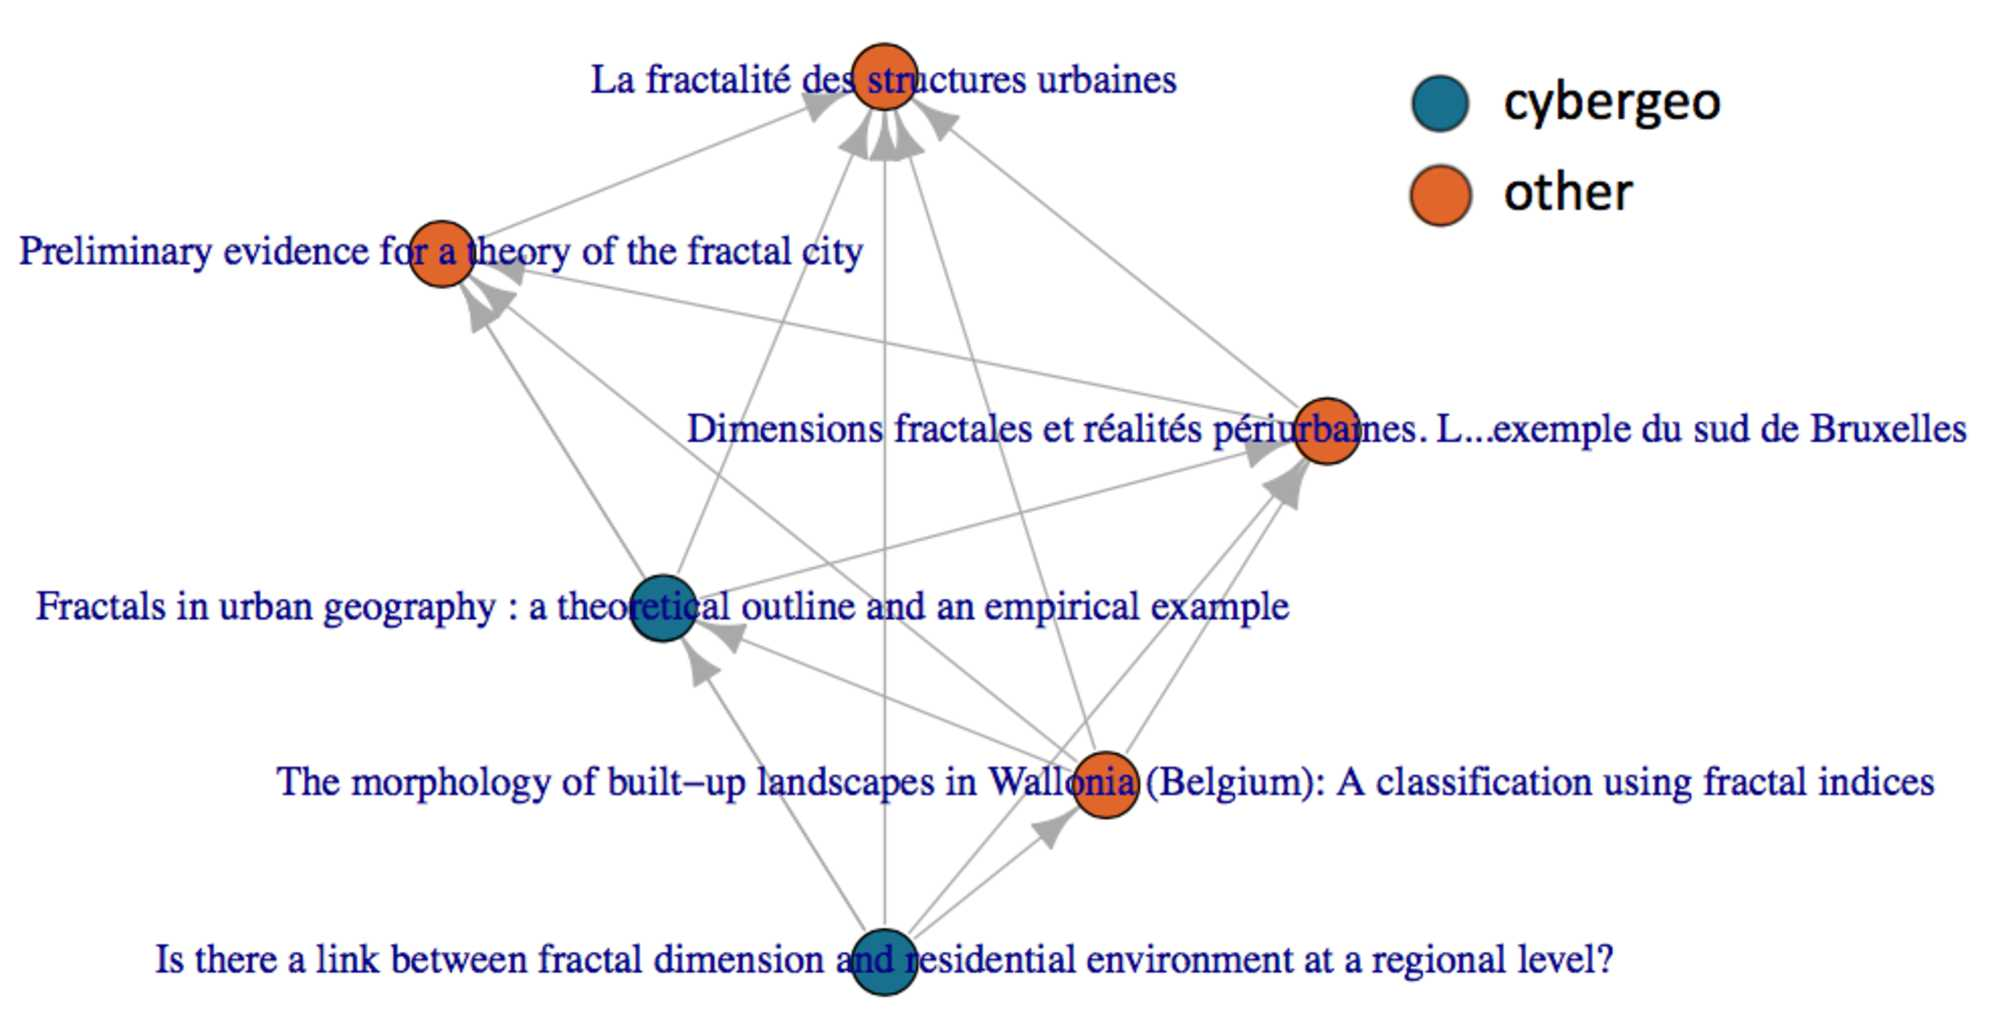
\includegraphics[width=\textwidth]{Figures/Cybergeo/Fig4.jpg}
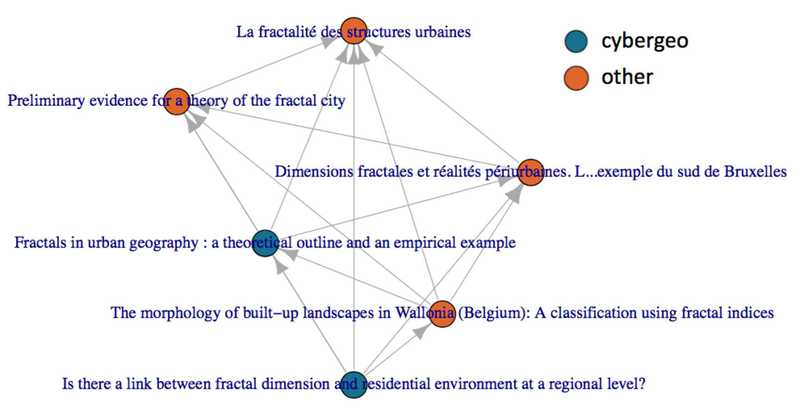
\includegraphics[width=\linewidth]{Figures/Final/B-cybergeo-fig4.jpg}
\appcaption{Example of a maximal clique in the citation network, paper of \texttt{Cybergeo} being in blue. Such topological structure reveal citation practices such as here a systematic citation of previous works in the research niche.\label{fig:cybergeo:fig4}}{\textbf{Exemple d'une clique maximale dans le réseau de citation.} Les articles de \textit{Cybergeo} sont en bleu. Une telle structure topologique révèle certaines pratiques de citation comme ici une citation systématique des travaux précédents dans la niche de recherche.\label{fig:cybergeo:fig4}}
\end{figure}
%%%%%%%%%%%%%%%%%



\paragraph{Citation communities}{Communautés de citation}

\bpar{
The citation network is a first opportunity to construct endogenous disciplines, by extracting citation communities. More precisely, this step aims at finding recurrent patterns in citations that would define a field by its citation practices. In order to be consistent with the particular data structure we have (missing incoming citations for sub-corpuses at maximal depth), we filter the network by removing all nodes with degree smaller than one. This ensures that kept nodes are either at least cited by an other node (and thus there are no missing edges for these nodes) or cite at least two other nodes, what can make ``bridges'' between sub-communities. The resulting network has a size of $\left|V\right| = 107164$ nodes and $\left|E\right| = 309778$ edges. It is visualized in Fig.~\ref{fig:cybergeo:fig5}.
}{
Le réseau de citation est une première opportunité pour construire des disciplines endogènes, par extraction des communautés de citation. Plus précisément, cette étape vise à identifier des motifs récurrents dans les citations, qui définiraient une discipline par ses pratiques de citation. Afin de rester cohérent avec la structure particulière de données que nous avons (citations entrantes manquantes pour les sous-corpus à profondeur maximale), nous filtrons le réseau en supprimant tous les noeuds de degré inférieur à 1. Cela assure que les noeuds restants sont soit au moins cités par un autre noeud (et donc il n'y a pas de liens manquants pour ces noeuds) ou citent au moins deux autre noeuds, ce qui peut faire des ``ponts'' entre sous-communautés. Le réseau obtenu a une taille de $\left|V\right| = 107164$ noeuds et $\left|E\right| = 309778$ liens. Celui-ci est visualisé en Fig.~\ref{fig:cybergeo:fig5}.
}


%%%%%%%%%%%%%%%%%
\begin{figure}
%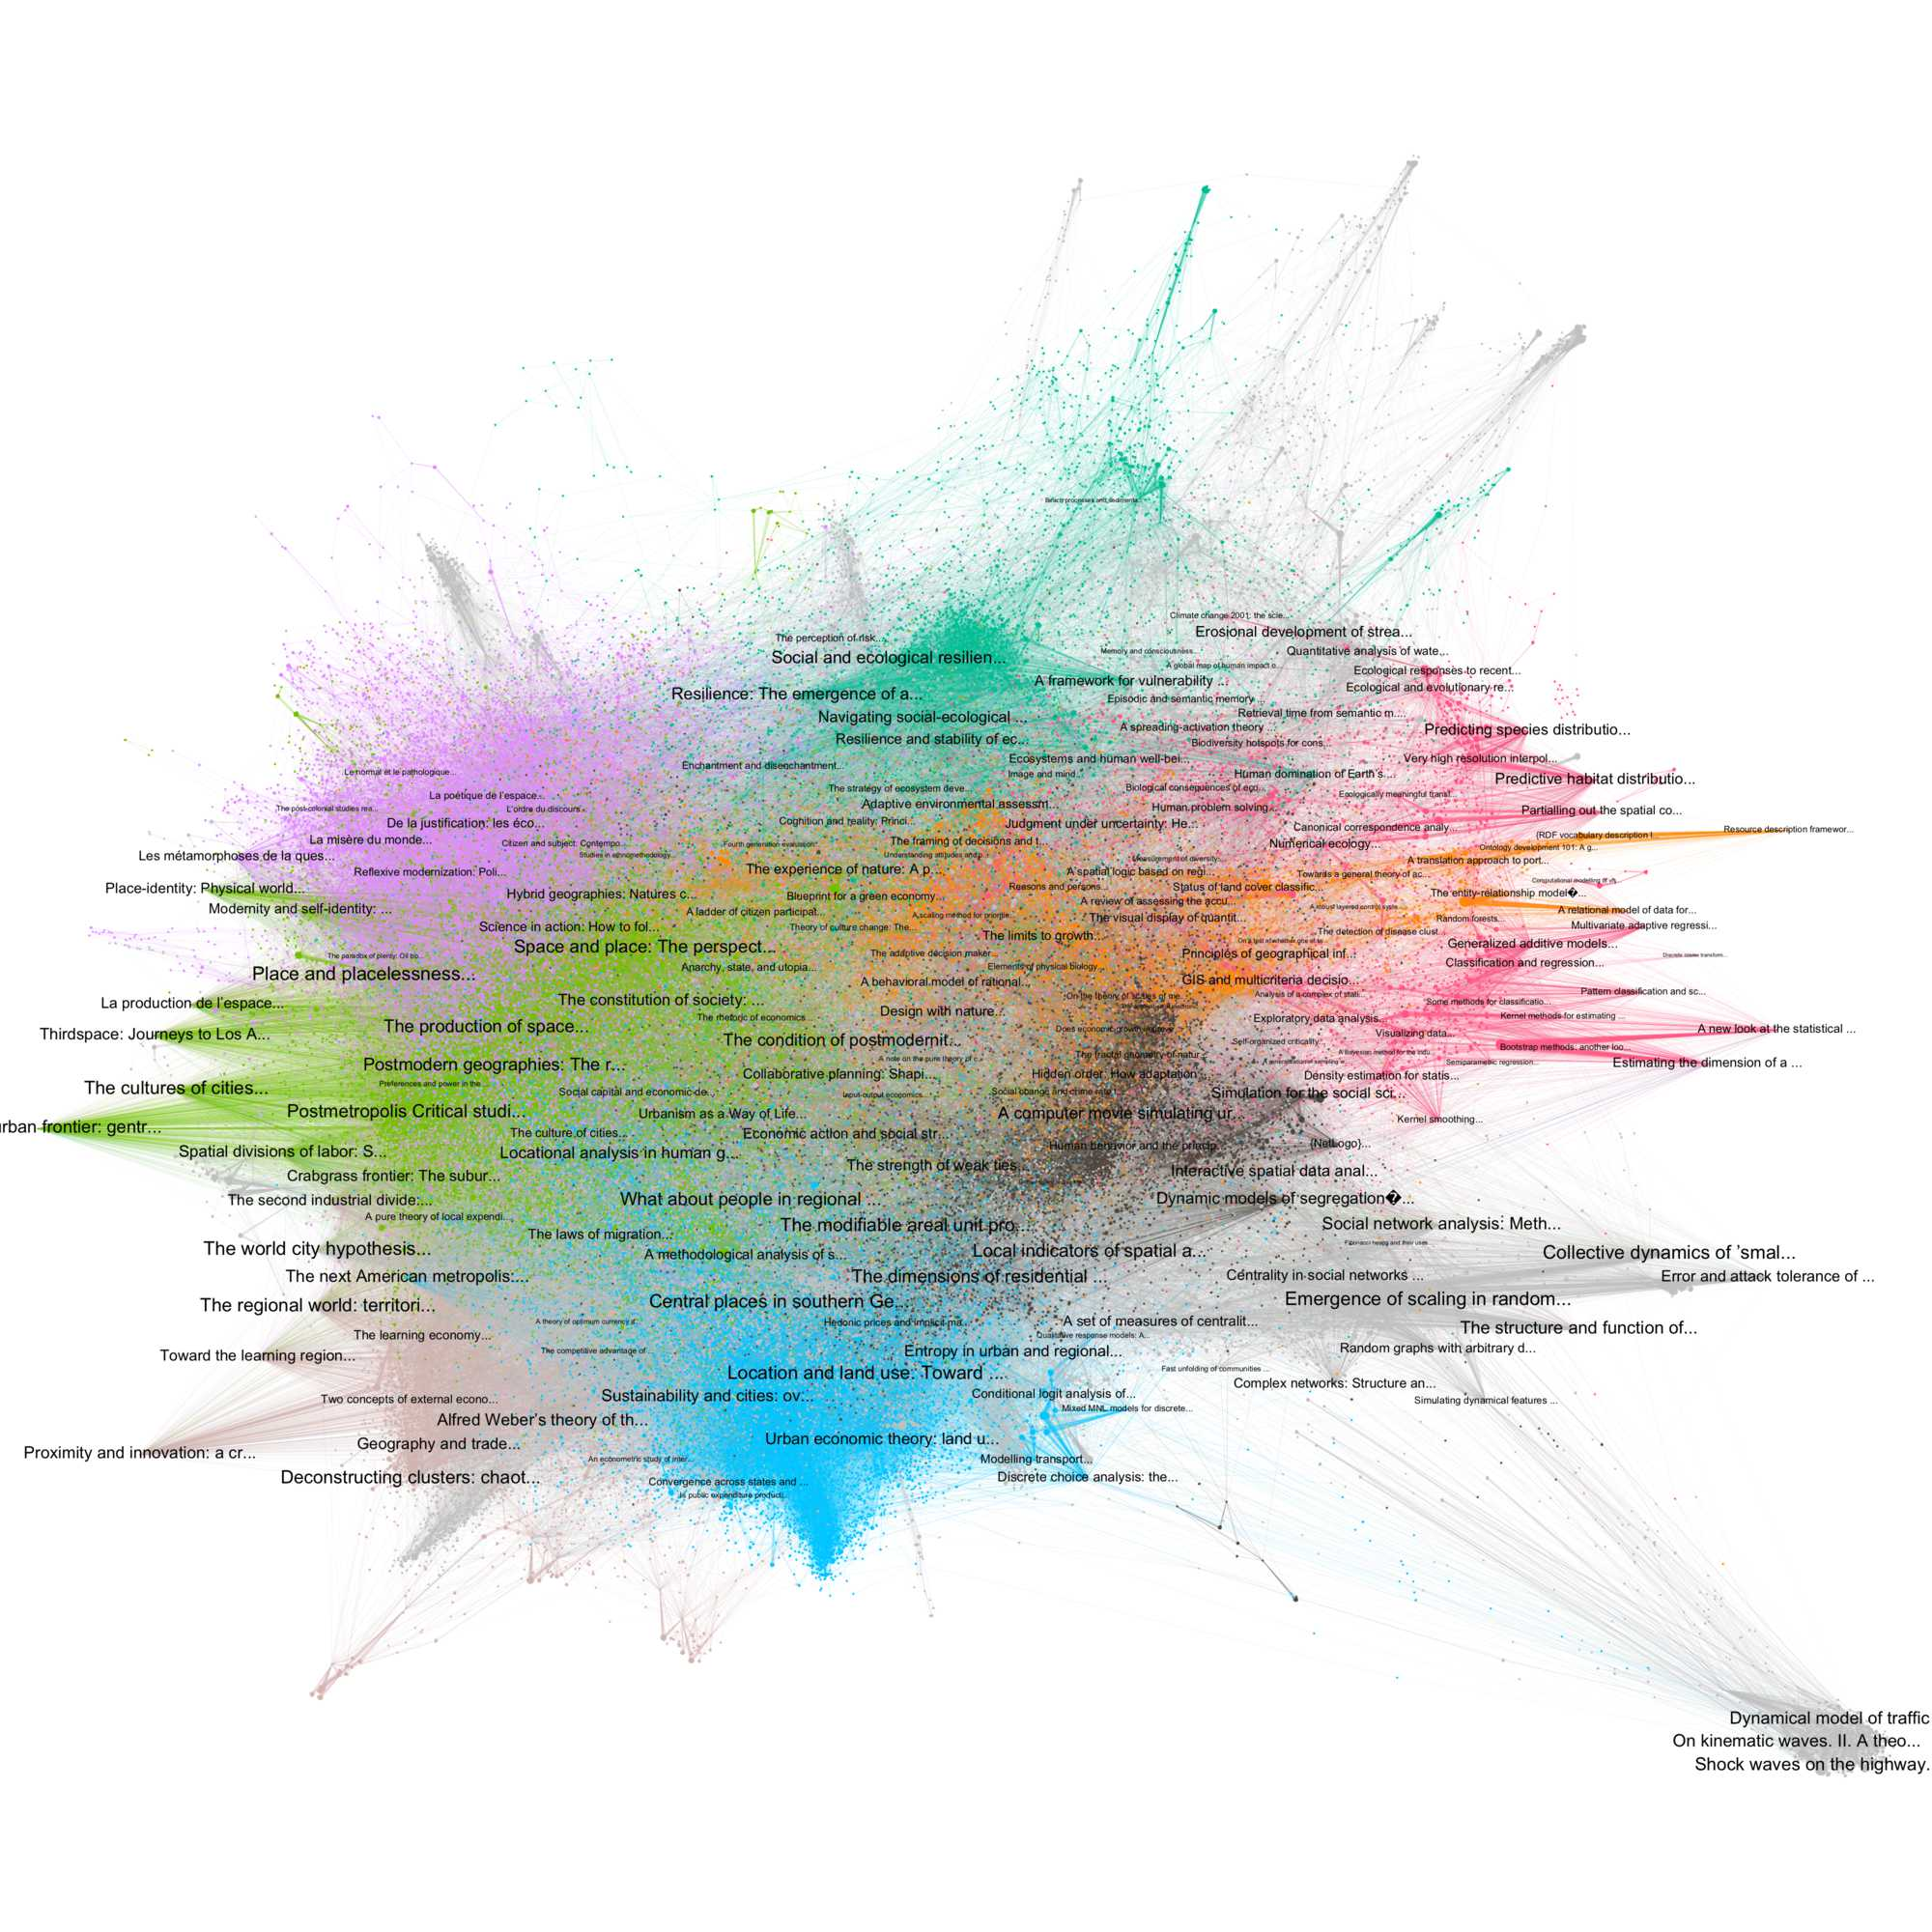
\includegraphics[width=\textwidth]{Figures/Cybergeo/Fig5.jpg}
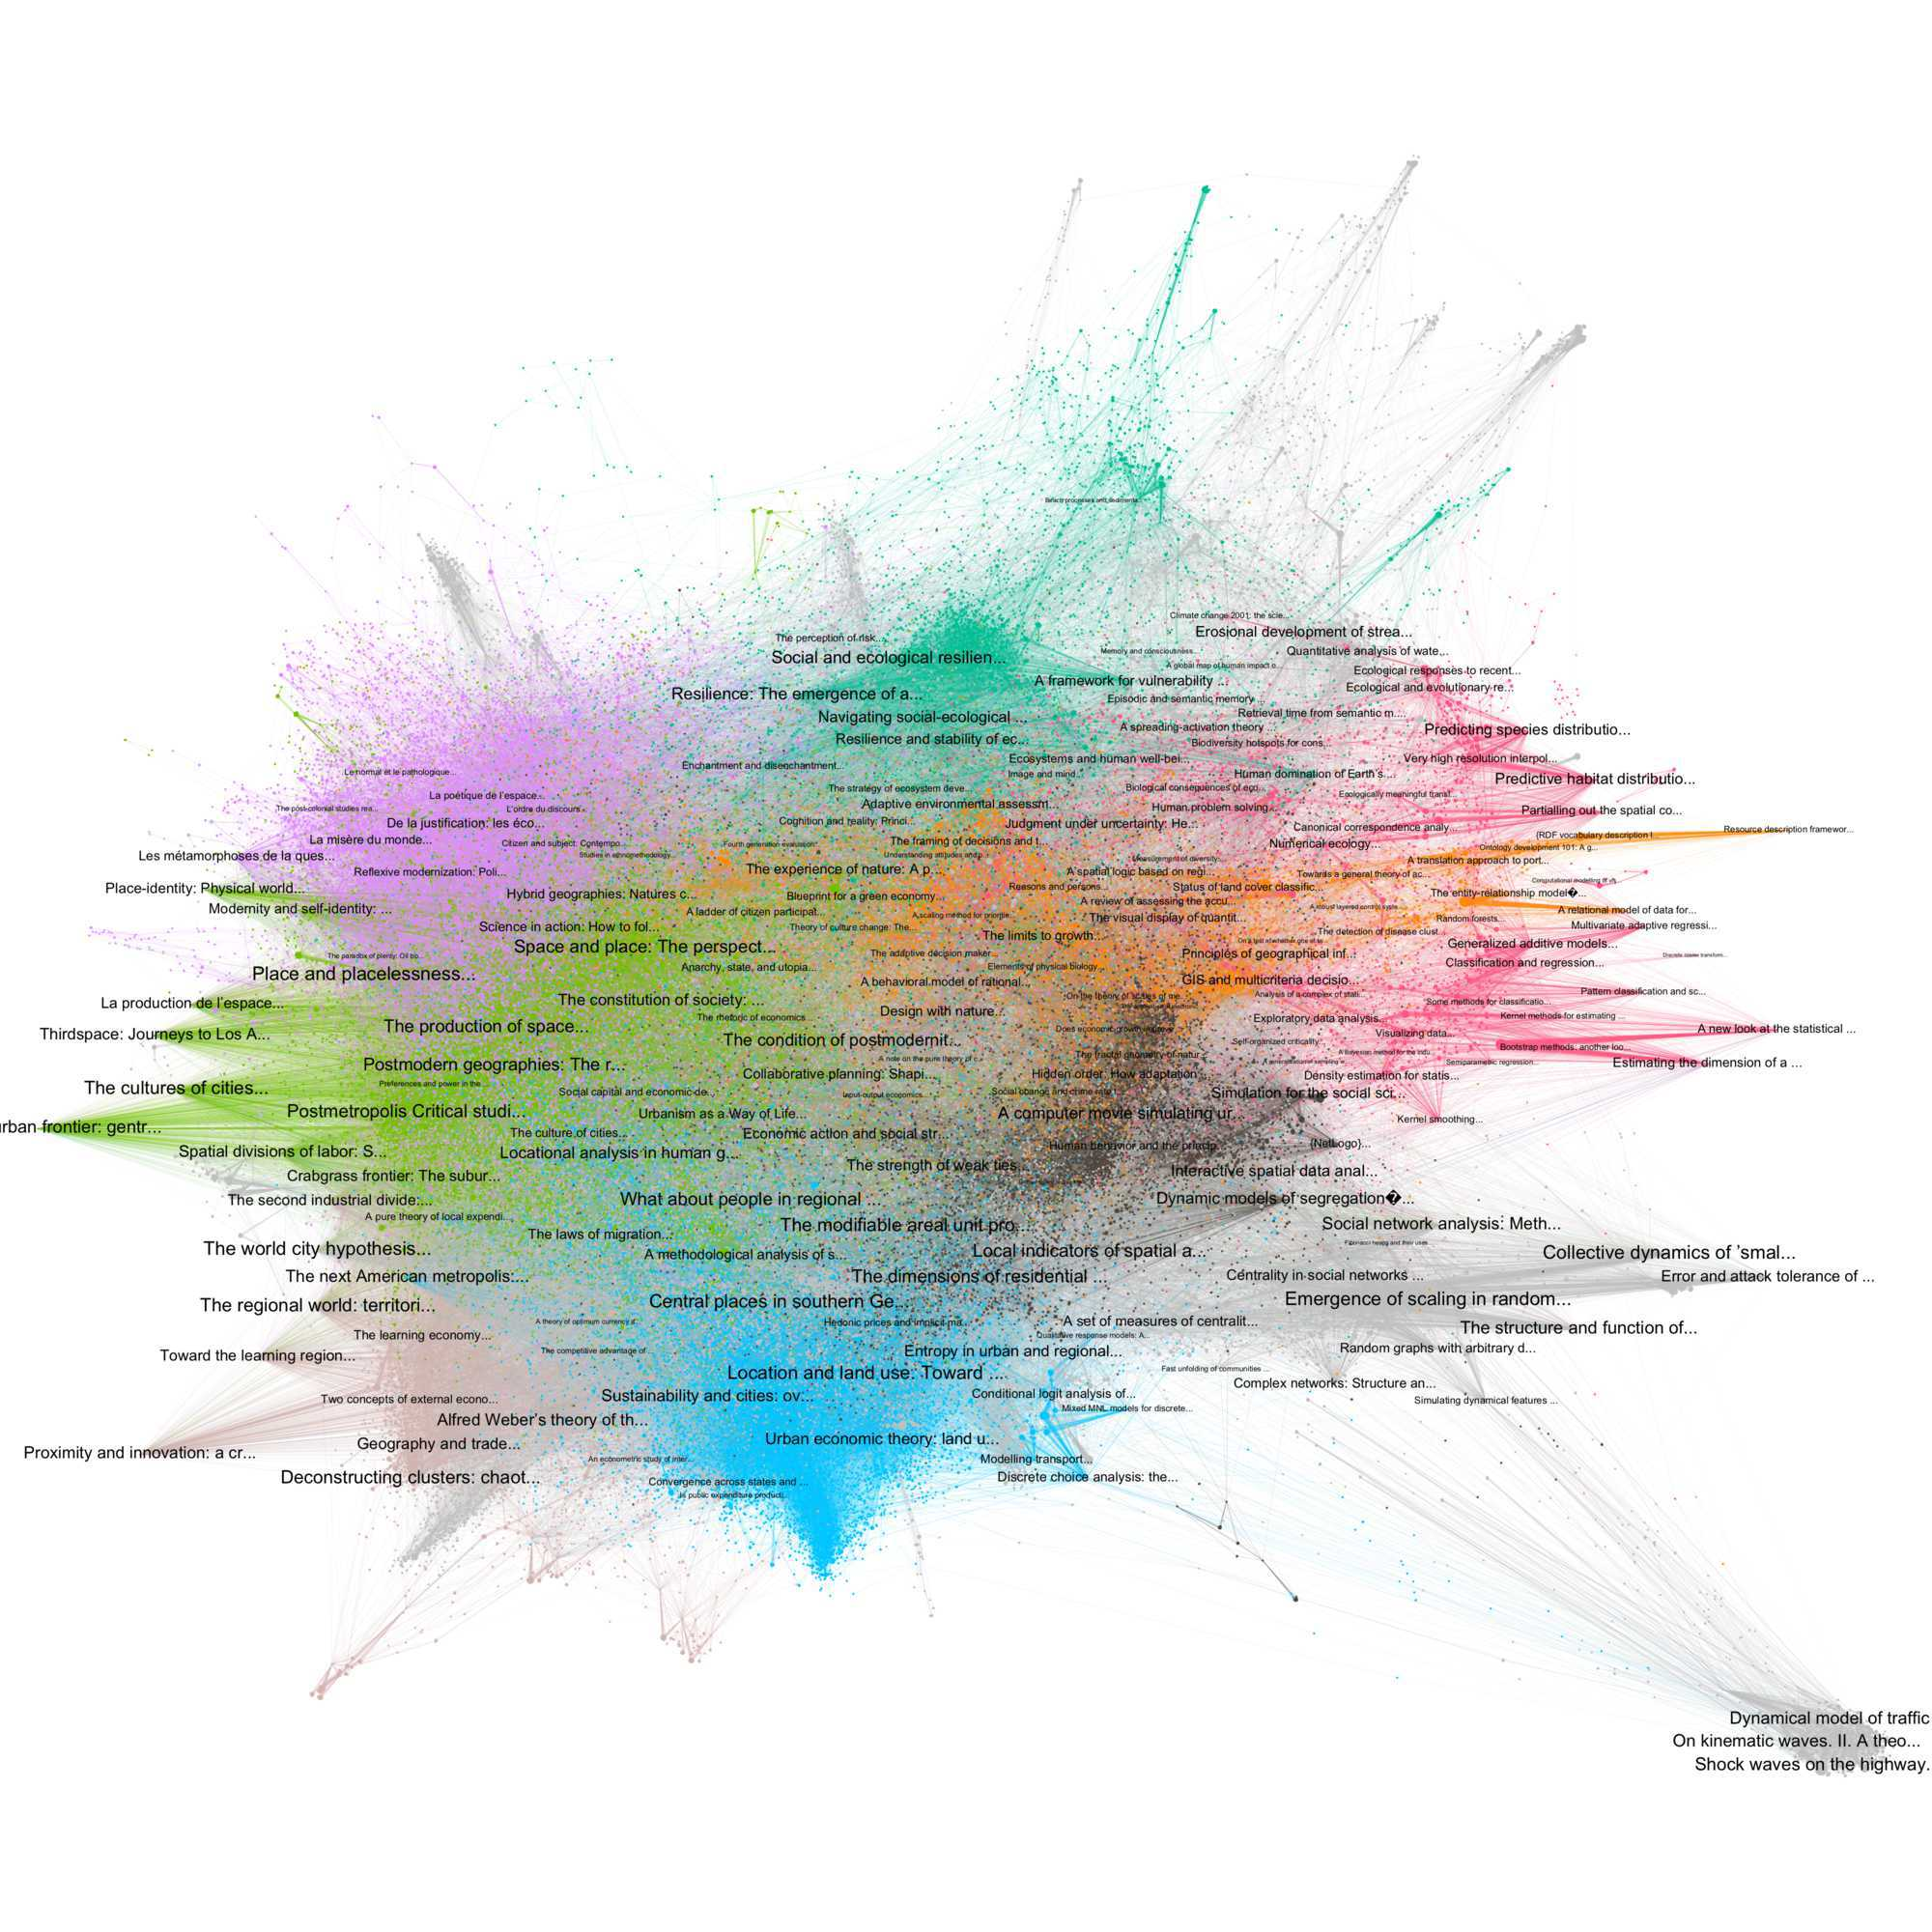
\includegraphics[width=\linewidth]{Figures/Final/B-cybergeo-fig5.jpg}
\appcaption{\textbf{Citation Network.} We show only the ``core'' of the citation network, composed by references with a degree larger than one ($\left|V\right| = 107164$ and $\left|E\right| = 309778$). The community detection algorithm provides 29 communities with a modularity of 0.71. Nodes and edges color gives the main communities (for example ecology in magenta, GIS in orange, Socio-ecology in turquoise, Social geography in green, Spatial analysis in blue). Node labels give shortened titles of most cited papers, size is scaled according to their in-degree. The graph is spatialized using a Force-Atlas algorithm.\label{fig:cybergeo:fig5}}{\textbf{Réseau de citations.} Nous visualisons uniquement le ``coeur'' du réseau de citation, composé des références avec un degré plus grand que 1 ($\left|V\right| = 107164$ et $\left|E\right| = 309778$). L'algorithme de détection de communautés fournit 29 communautés avec une modularité de 0.71. Les couleurs des noeuds et des liens donnent les communautés principales (par exemple l'écologie en magenta, GIS en orange, la Socio-écologie en turquoise, la géographie sociale en vert, l'analyse spatiale en bleu). Les labels des noeuds donnent les titres raccourcis des références les plus citées, la taille étant à l'échelle de leur degré entrant. Le graphe est spatialisé par l'utilisation d'un algorithme Force-Atlas.\label{fig:cybergeo:fig5}}
\end{figure}
%%%%%%%%%%%%%%%%%


\bpar{
We use a standard modularity optimization algorithm to identify communities~\citep{blondel2008fast} in this citation network. It provides 29 communities with a modularity of 0.71. In comparison, a bootstrap of 100 randomisations of links in the network gives an average modularity of $-1.0\cdot 10^{-4} \pm 4.4\cdot 10^{-4}$ which means that communities are highly significant.
}{
Nous utilisons un algorithme standard d'optimisation de modularité pour identifier des communautés~\citep{blondel2008fast} dans ce réseau de citation. Il fournit 29 communautés avec une modularité de 0.71. En comparaison, un bootstrap de 100 tirages aléatoires des liens dans le réseau donne une modularité moyenne de $-1.0\cdot 10^{-4} \pm 4.4\cdot 10^{-4}$ ce qui signifie une forte significativité des communautés.
}

\bpar{
We name the communities by inspection of the titles of most cited references in each. The 14 communities that have a size larger than 2.5\% of the network are : Complex Networks, Ecology, Social Geography, Sociology, GIS, Spatial Analysis, Agent-based Modeling and Simulation (ABMS), Socio-ecology, Urban Networks, Urban Simulation, Urban Studies, Economic Geography, Accessibility/Land-use, Time Geography. These categories do not directly correspond to well-defined disciplines, as some correspond more to methods (ABMS), objects of study (Urban Studies), or paradigms (Complex Networks). Some are ``specializations'' of others : most papers in Urban Studies can also be classified as Critical and Social geography. This way, we construct endogenous disciplines that correspond to \emph{scientific practices} (what is cited) more than their representation (the ``official'' disciplines). The relative positioning of communities in Fig.~\ref{fig:cybergeo:fig5}, obtained with a Force-Atlas algorithm, tells a lot about their respective relations : for example, social geography makes a bridge between Urban Studies and Economic Geography, whereas the connection between Socio-ecology and Urban simulations is done by GIS (what can be expected as geomatics is an interdisciplinary field). GIS also separates and connects two subfield of Ecology, on one side more thematic studies on ecological habitats, and on the other sides statistical methods. These relations already inform qualitatively patterns of interdisciplinarity, in the sense of integration measures. We will also in the following use these communities to situate the semantic classification.
}{
Nous nommons les communautés par inspection des titres des références les plus citées dans chaque. Les 14 communautés qui ont une taille plus grande que 2.5\% du réseau sont : \textit{Complex Networks, Ecology, Social Geography, Sociology, GIS, Spatial Analysis, Agent-based Modeling and Simulation (ABMS), Socio-ecology, Urban Networks, Urban Simulation, Urban Studies, Economic Geography, Accessibility/Land-use, Time Geography}. Ces catégories ne correspondent par directement à des disciplines bien définies, puisque certaines correspondent plus à des méthodes (\textit{ABMS}), des objets d'étude (\textit{Urban Studies}), ou des paradigmes (\textit{Complex Networks}). Certains sont des ``spécialisations'' d'autres : la plupart des travaux en \textit{Urban Studies} peuvent aussi être classifiés comme géographie critique ou sociale. De cette façon, nous construisons des disciplines endogènes qui correspondent à des \emph{pratiques scientifiques} (ce qui est cité) plus qu'à leur représentations (les disciplines ``officielles''). Le positionnement relatif des communautés en Fig.~\ref{fig:cybergeo:fig5}, obtenu par un algorithme de Force-Atlas, en dit long sur leurs relations respectives : par exemple la géographie sociale fait une pont entre les \textit{Urban Studies} et l'économie géographique, tandis que la connection entre socio-écologie et les simulations urbaines est fait par le GIS (ce qui pouvait être attendu car la géomatique est un champ interdisciplinaire). Le GIS sépare également et connecte deux sous-champs de l'écologie, d'une part des études plus thématiques sur les habitats écologiques, et d'autre part des méthodes statistiques. Ces relations informent déjà qualitativement des motifs d'interdisciplinarité, au sens de mesures d'intégration. Nous allons par la suite utiliser ces communautés pour situer la classification sémantique.
}




%%%%
% Core properties :
% |V| = 107164
% |E| = 309778
% Modularity = 0.694



% "Community 24 ; corpus prop 2.12291441155612"
%17103773263010692469                                             Shock waves on the highway    704
%5930190645967036557                              Traffic dynamics: studies in car following    531
%6454619432004957861  On kinematic waves. II. A theory of traffic flow on long crowded roads    671
%15823582570548231219         Dynamical model of traffic congestion and numerical simulation    673
%[1] "Community 10 ; corpus prop 4.16557799260946"
%15243168274213127296                  Social network analysis: Methods and applications    658
%10638755925462666384                            Emergence of scaling in random networks    756
%4992186057191694547  Collective dynamics of \342\200\231small-world\342\200\231networks    758
%12945060519911641528                     The structure and function of complex networks    687
%[1] "Community 16 ; corpus prop 4.81318353178306"
%13398523337335518206                         Predictive habitat distribution models in ecology    566
%13467121252331935431                                               Generalized additive models    418
%11029642873510533673 Predicting species distribution: offering more than simple habitat models    562
%13831040667378725133                                       Estimating the dimension of a model    454
%[1] "Community 17 ; corpus prop 11.8743234668359"
%6052144816936635558                                        Pour une g\303\251ographie du pouvoir    478
%9980715752622498273                      Les mots de la g\303\251ographie: dictionnaire critique    590
%14304156646457097003                    De la justification: les \303\251conomies de la grandeur    440
%2870436522105960522   Les m\303\251tamorphoses de la question sociale: une chronique du salariat    458
%[1] "Community 18 ; corpus prop 5.57556642155948"
%6414662845457641721   The constitution of society: Outline of the theory of structuration    593
%4337430435041504651  Modernity and self-identity: Self and society in the late modern age    493
%7898783771677764446                                        The condition of postmodernity    658
%7835092538327027347     Economic action and social structure: the problem of embeddedness    516
%[1] "Community 6 ; corpus prop 3.60475532828189"
%                                                          titles degree
%12482866708510596998                           The power of maps    575
%1164911542533093357      GIS and multicriteria decision analysis    463
%16457974396311846489  Spatial behavior: A geographic perspective    552
%2954521275884877195                       Deconstructing the map    631
%[1] "Community 3 ; corpus prop 5.13885259975365"
%11531103519383816169 The structure and growth of residential neighborhoods in American cities    692
%62057246354689685                                                        The nature of cities    713
%3545913291616437667                                   Locational analysis in human geography.    627
%17899222184184316747                                       Central places in southern Germany    740
%[1] "Community 14 ; corpus prop 6.66735097607405"
%12954335397668543979  Cellular automata and fractal urban form: a cellular modelling approach to the evolution of urban land-use patterns
%4133663650988164381                                                                       Fractal cities: a geometry of form and function
%1594743421920318397                                                       Growing artificial societies: social science from the bottom up
%14559759739366955015                                   Multi-agent systems for the simulation of land-use and land-cover change: a review
%                     degree
%12954335397668543979    743
%4133663650988164381     747
%1594743421920318397     604
%14559759739366955015    778
%[1] "Community 9 ; corpus prop 1.9829420327722"
%1594126764449801706                                                               Quantitative analysis of watershed geomorphology
%8328827169345207094  Erosional development of streams and their drainage basins; hydrophysical approach to quantitative morphology
%8539006751955791402                                                                              Statistical law of stream numbers
%12081487864131557751                                                  Hypsometric (area-altitude) analysis of erosional topography
%                     degree
%1594126764449801706     382
%8328827169345207094     536
%8539006751955791402     391
%12081487864131557751    408
%[1] "Community 27 ; corpus prop 0.851032063006233"
%10726714213083688457                                Transmission dynamics of the etiological agent of SARS in Hong Kong: impact of public health interventions
%3970869213781401070  Impact of climatic change on the northern latitude limit and population density of the disease-transmitting European tick Ixodes ricinus.
%2455775719744402150                                   Epidemiological determinants of spread of causal agent of severe acute respiratory syndrome in Hong Kong
%8395695762893339661                                                                     Transmission dynamics and control of severe acute respiratory syndrome
%                     degree
%10726714213083688457    475
%3970869213781401070     116
%2455775719744402150     216
%8395695762893339661     430
%[1] "Community 8 ; corpus prop 0.733455264827741"
%932712685133827561   The physiological equivalent temperature\342\200\223a universal index for the biometeorological assessment of the thermal environment
%1480142480183496272                                                                                                                      The urban climate
%17024728103875347383                             A field study of thermal comfort in outdoor and semi-outdoor environments in subtropical Sydney Australia
%833745332327046870                                                         Applications of a universal thermal index: physiological equivalent temperature
%                     degree
%932712685133827561      391
%1480142480183496272     173
%17024728103875347383    153
%833745332327046870      293
%[1] "Community 21 ; corpus prop 6.45272666193871"
%12312403172976436756                                          Social and ecological resilience: are they related?
%932477214288257460   Resilience: The emergence of a perspective for social\342\200\223ecological systems analyses
%5340448582567072501                                     From metaphor to measurement: resilience of what to what?
%1509391713535671469           Navigating social-ecological systems: building resilience for complexity and change
%                     degree
%12312403172976436756    665
%932477214288257460      646
%5340448582567072501     651
%1509391713535671469     579
%[1] "Community 13 ; corpus prop 3.00474039789482"
%                                                           titles degree
%12568908445725112885                             The world cities    629
%14432190559149797085                     A roster of world cities    581
%3966620121471250312   World city network: a global urban analysis    716
%7479248257935000396                     The world city hypothesis    760
%
%[1] "Community 23 ; corpus prop 5.62875592549737"
%3553655105619346230                                                                  The modifiable areal unit problem
%14305556346317738837  A million or so correlation coefficients: three experiments on the modifiable areal unit problem
%15192663253141002697                                    A computer movie simulating urban growth in the Detroit region
%2556056281630746501                                                       Local indicators of spatial association-LISA
%                     degree
%3553655105619346230     741
%14305556346317738837    661
%15192663253141002697    643
%2556056281630746501     724
%[1] "Community 2 ; corpus prop 9.9660333694151"
%                                                                        titles degree
%12738968557765837578                                    The cultures of cities    732
%13746171706822239563     Postmetropolis Critical studies of cities and regions    715
%2116873643451406893   Fortress America: gated communities in the United States    704
%14292387866086321708                                   Place and placelessness    760
%[1] "Community 22 ; corpus prop 7.13579187040424"
%                                                                              
%11080283063311825032  The regional world: territorial development in a global economy    740
%3554088320531351693                                        Location and space-economy    719
%7086787680145296542       Deconstructing clusters: chaotic concept or policy panacea?    726
%[1] "Community 28 ; corpus prop 1.4379829047068"
%
%16044574669948655149     Saharan dust contributions to PM10 and TSP levels in Southern and Eastern Spain
%8425362340869409578   Climats, for\303\252ts et d\303\251sertification de l\342\200\231Afrique tropicale
%1129714354835431503                                                    Nonparametric tests against trend
%1135676043916984792                                A non-parametric approach to the change-point problem
%                     degree
%16044574669948655149    144
%8425362340869409578     160
%1129714354835431503     181
%1135676043916984792     203
%[1] "Community 1 ; corpus prop 1.67500279944758"
%                                                               titles degree
%1627107393903704279         The dimensions of residential segregation    724
%4099483990695182730                             Models of segregation    466
%747074237233961749          Dynamic models of segregation\342\200\240    622
%18105468109972109903 A methodological analysis of segregation indexes    506
%[1] "Community 5 ; corpus prop 9.77847038184465"
%                                                                           titles degree
%13956442331799241731 Location and land use. Toward a general theory of land rent.    748
%15575741556156415962                            How accessibility shapes land use    782
%13897256231045447464                                      Urban spatial structure    783
%5192159686471589942                 Are compact cities a desirable planning goal?    741
%[1] "Community 26 ; corpus prop 1.98760777873166"
%12131824341349033633                                              Connectivity is a vital element of landscape structure
%15969739511774356860      The application of \342\200\231least-cost\342\200\231modelling as a functional landscape model
%3875238890909508946  Promoting ecosystem and human health in urban areas using green infrastructure: a literature review
%15970185536531379583                                                                   Ecosystem services in urban areas
%                     degree
%12131824341349033633    343
%15969739511774356860    262
%3875238890909508946     265
%15970185536531379583    319
%[1] "Community 4 ; corpus prop 1.24575417117689"
%                                                                      titles degree
%17518815146409301085                       Visual methods in social research    309
%3130282044894438080                 Image as a factor in tourism development    222
%6005112106352993762   Understanding and measuring tourist destination images    211
%17773583015280146421    Talking about pictures: A case for photo elicitation    412
%
%[1] "Community 11 ; corpus prop 2.66134149527827"
%15987432381426193038                                                                                           Time in geographic information systems
%4916773650386052166  It\342\200\231s about time: A conceptual framework for the representation of temporal dynamics in geographic information systems
%10741249551199253506                                                                                 A spatial logic based on regions and connection.
%1707686457311089380                                       An event-based spatiotemporal data model (ESTDM) for temporal analysis of geographical data
%                     degree
%15987432381426193038    557
%4916773650386052166     399
%10741249551199253506    339
%1707686457311089380     388
%[1] "Community 12 ; corpus prop 0.0541226531297824"
%
%320633167171028945   \342\200\231Unite Unite Europe\342\200\231The political and cultural structures of Europe as reflected in the Eurovision Song Contest
%8402251348308572830          Comparison of Eurovision Song Contest simulation with actual results reveals shifting patterns of collusive voting alliances.
%2610553645533349879                                                       Save the last dance for me: Unwanted serial position effects in jury evaluations
%10488781352782564265                                                  Save the last dance II: Unwanted serial position effects in figure skating judgments
%                     degree
%320633167171028945       25
%8402251348308572830      24
%2610553645533349879      32
%10488781352782564265     18
%[1] "Community 25 ; corpus prop 0.747452502706133"
%                                                         titles degree
%5749645930528845292           Theorising the rise of regionness     89
%16110139515439702034          The geographical pivot of history    232
%18249508238183354137                            Arctic meltdown     57
%15128616333100707022  Geography and politics in a world divided    112
%[1] "Community 29 ; corpus prop 0.570154156246501"
%
%17875356408399137122 The second demographic transition in Western countries: An interpretation    361
%9773560585688720648                          Europe\342\200\231s second demographic transition    422
%4173326927865475733              La famille en Europe occidentale: divergences et convergences     79
%5987517425216101496                        Family ties in Western Europe: persistent contrasts    248
%[1] "Community 20 ; corpus prop 0.0718524877757456"
%                                                                                                                                    
%18395417624936874618                                                                The development crisis in Vietnam\342\200\231s mountains
%269325805179871458    Doi Moi in the mountains: land use changes and farmers\342\200\231 livelihood strategies in Bac Kan Province, Viet Nam
%8071930996413902082                                                                   Choosing rural road investments to help reduce poverty
%5647127754479004480                                           The spatial distribution of poverty in Vietnam and the potential for targeting
%                     degree
%18395417624936874618     29
%269325805179871458       37
%8071930996413902082      34
%5647127754479004480      17
%
%[1] "Community 7 ; corpus prop 0.0261281773729984"
%5883716409547177886 All or none: no stable hybrid or half-way solutions for launching the learned periodical literature into the postGutenberg galaxy
%9133434386405239110                                                                                         Web journals publishing: a UK perspective
%6281042621755024923                                                                                                 The invisible hand of peer review
%2432100162443594098                                                                             Electronic publishing takes journals into a new realm
%                    degree
%5883716409547177886     19
%9133434386405239110      5
%6281042621755024923     18
%2432100162443594098      4
%
%[1] "Community 15 ; corpus prop 0.0083983427270352"
%[1] titles degree
%<0 rows> (or 0-length row.names)
%
%[1] "Community 19 ; corpus prop 0.0177298346459632"
%15912331793517931633 Les discriminations selon l\342\200\231origine dans l\342\200\231acc\303\250s aux soins
%2939440609801692906                          Etat de sant\303\251 des populations immigr\303\251es en France
%695207205763025392                                         Entre droit aux soins et qualit\303\251 des soins
%1837393795895317408               Sant\303\251 et immigration. Les v\303\251rit\303\251s politiques du corps
%                     degree
%15912331793517931633      7
%2939440609801692906       5
%695207205763025392        5
%1837393795895317408       5
%
%










%%%%%%%%%%%%%%%%%%
\subsubsection{Semantic Communities Construction}{Construction des communautés sémantiques}

\bpar{
We now turn to the methodological details for the construction of the semantic classification. This step adapts the methodology described by~\cite{bergeaud2017classifying}, who construct a semantic classification on patent data.
}{
Nous présentons à présent les détails méthodologiques de la construction de la classification sémantique. Cette étape adopte la méthodologie décrite par~\cite{bergeaud2017classifying}, qui construit une classification sémantique sur données de brevets.
}


%%%%%%%%%%%%%%%%%%
\paragraph{Relevant Keywords Extraction}{Extraction des Mots-clés pertinents}

\bpar{
We recall that our corpus with available text consists of around $2\cdot 10^5$ abstracts of publications at a topological distance shorter than 2 from the journal \textit{Cybergeo} in the citation network. The first important step is to extract relevant keywords from abstracts. Text processing is done with the python library \texttt{nltk}~\citep{bird2006nltk}. We add a particular treatment to the method of~\cite{bergeaud2017classifying}, as our corpus is multilingual: language detection is done with the technique of \emph{stop-words}~\citep{baldwin2010language}. We also use a specific tagger (the function allowing the attribution of grammatical function to words), \texttt{TreeTagger}~\citep{schmid1994probabilistic}, for languages other than English.
}{
Nous rappelons que notre corpus avec des textes disponibles consiste en environ $2\cdot 10^5$ résumés des publications à une distance topologique plus petite que 2 du journal \textit{Cybergeo} dans le réseau de citation. La première étape importante est l'extraction de mots-clés pertinents à partir des résumés. L'analyse textuelle est effectué avec la bibliothèque python \texttt{nltk}~\cite{bird2006nltk}. Nous ajoutons un traitement particulier à la méthode de~\cite{bergeaud2017classifying}, puisque notre corpus est multilingue : la détection de langue est faite par technique des \emph{stop-words}~\citep{baldwin2010language}. Nous utilisons également un tagger spécifique (la fonction permettant l'attribution de fonctions grammaticales aux mots), \texttt{TreeTagger}~\citep{schmid1994probabilistic}, pour les langues autres que l'anglais.
}

\bpar{
To summarize, the keyword extraction workflow goes through the following steps :
}{
En résumé, le flux d'extraction des mots-clés suit les étapes suivantes :
}

\bpar{
\begin{enumerate}
\item Language detection is done using \textit{stop-words}
\item Pos-tagging (detection of word functions) and stemming (extraction of the \emph{stem}) are done differently depending on language :
\begin{itemize}
\item English : \texttt{nltk} built-in pos-tagger, combined to a \emph{PorterStemmer}
\item French or other : use of \texttt{TreeTagger}~\citep{schmid1994probabilistic}
\end{itemize}
\item Selection of potential \textit{n-grams} (keywords of length $n$ with $1 \leq n \leq 4$) following the given grammatical rules: for English $\bigcap \{NN \cup VBG \cup JJ \}$, and for French $\bigcap \{NOM \cup ADJ\}$. Other languages are a negligible proportion of the corpus and are discarded.
\item Estimation of the relevance \textit{n-grams}, by attributing a score following the deviation of the statistical distribution of co-occurrences to a random distribution.
\end{enumerate}
}{
\begin{enumerate}
	\item La détection de la langue est faite par utilisation des \textit{stop-words}
	\item Le \emph{pos-tagging} (détection des fonctions des mots) et le \emph{stemming} (extraction du \emph{stem}) sont effectués différemment selon la langue :
	\begin{itemize}
		\item Anglais : \emph{pos-tagger} intégré à \texttt{nltk}, combiné à un \emph{PorterStemmer}
		\item Français ou autre : utilisation de \texttt{TreeTagger}~\citep{schmid1994probabilistic}
	\end{itemize}
	\item Sélection de \textit{n-grams} potentiels (mots-clés de longueur $n$ avec $1 \leq n \leq 4$) suivant les règles grammaticales données : pour l'anglais $\bigcap \{NN \cup VBG \cup JJ \}$, et pour le français $\bigcap \{NOM \cup ADJ\}$. Les autres langues sont une proportion négligeable du corpus et ne sont pas pris en compte.
	\item Estimation de la pertinence des \textit{n-grams}, par attribution d'un score suivant la déviation des distribution statistiques des co-occurrences à une distribution aléatoire.
\end{enumerate}
}


%%%%%%%%%%%%%%%%%%
\paragraph{Semantic Network}{Réseau sémantique}

\bpar{
We keep at this stage a fixed number $K_W$ of \textit{n-grams}, based on their relevance score, that will be designated as the relevant keywords. We find that for large values of $K_W$, results are not sensitive to the total number of keywords, and take a reasonably large value for computational performance, $K_W = 50,000$. We construct the co-occurrence matrix of the relevant keywords. This co-occurrence matrix provides the semantic network as its adjacency matrix : nodes are keywords, and they are linked according to their co-occurrences.
}{
Nous conservons à cette étape un nombre fixé $K_W$ de \textit{n-grams}, en se basant sur leur score de pertinence, qui seront désignés comme mots-clés pertinents. Nous observons que pour des grandes valeurs de $K_W$, les résultats ne sont pas sensibles au nombre total de mots-clés, et prenons ainsi une grande valeur raisonnable pour la performance computationnelle, $K_W = 50,000$. Nous construisons la matrice de co-occurrence des mots-clés pertinents. Cette matrice de co-occurrence fournit le réseau sémantique comme sa matrice d'adjacence : les noeuds sont les mots-clés, et ils sont reliés en fonction de leurs co-occurrences.
}


%%%%%%%%%%%%%%%%%%
\paragraph{Sensitivity Analysis}{Analyse de sensibilité}

\bpar{
We observe the same phenomenon than in~\cite{bergeaud2017classifying}, that is the existence of nodes with large degree and not specific to a particular field : for example \texttt{model} and \texttt{space} are used in most of subfields of Geography. We also adapt the original filtering procedure, as we do not have here an exogenous information to calibrate parameters. We assume the highest degree terms do not carry specific information on particular classes and can be thus filtered given a maximal degree threshold $k_{max}$. We keep the second filter on a minimal edge weight threshold $\theta_w$. We add the supplementary constraint that keywords are also filtered on a document frequency window $\left[ f_{min},f_{max} \right]$ (number of references in which they appear), what is slightly different from network filtering.
}{
Nous observons un phénomène similaire à celui observé par~\cite{bergeaud2017classifying}, qui est la présence de noeuds avec un grand degré mais non spécifiques à un champ particulier : par exemple \texttt{model} et \texttt{space} sont utilisés dans la majorité des sous-champs de la Géographie. Nous adaptons également la procédure de filtration originale, puisque nous ne disposons pas ici d'information exogène pour calibrer les paramètres. Nous supposons que les termes de plus haut degré ne portent pas d'information sur des classes en particulier et peuvent ainsi être filtrés étant donné un degré maximal $k_{max}$. Nous gardons le second filtre sur un seuil de poids minimal des liens $\theta_w$. Nous ajoutons la contraintes supplémentaires que les mots-clés sont aussi filtrés par leur fréquence d'apparition dans les documents sur une fenêtre $\left[ f_{min},f_{max} \right]$ (nombre de références dans lesquelles ils apparaissent), ce qui est légèrement différent de la filtration du réseau.
}


\bpar{
A sensitivity analysis of resulting network topology to these four parameters is presented in Fig.~\ref{fig:cybergeo:fig6}. Given a filtered network, we detect communities using modularity optimization as before for the citation network. Various properties of the network can be optimized, and we look in particular at its size (number of keywords after filtering), the optimal modularity, the number of communities, and the balance between their sizes (defined as a concentration index $\sum_k s_k^2 / (\sum_k s_k)^2$). This multi-objective optimization problem does not have a unique solution as objectives are contradictory in a complex way, and a compromise point must be chosen. We take a compromise point between modularity and network size, with a high balance and a reasonable number of communities, given by $k_{max} = 1200, \theta_w = 100, f_{min} = 50, f_{max} = 10000$. These values give a network of size 2868, with 18 communities and a modularity of 0.57.
}{
Une analyse de sensibilité de la topologie du réseau résultant à ces quatre paramètres est présentée en Fig.~\ref{fig:cybergeo:fig6}. Etant donné un réseau filtré, nous détectons les communautés en utilisant une optimisation de la modularité comme ci-dessus pour le réseau de citation. Diverses propriétés du réseau peuvent être optimisées, et nous nous intéressons en particulier à sa taille (nombre de mots-clés après filtrage), la modularité optimale, le nombre de communautés, et l'équilibre entre leurs tailles (défini comme un indice de concentration $\sum_k s_k^2 / (\sum_k s_k)^2$). Ce problème d'optimisation multi-objectif ne possède pas de solution unique car les objectifs sont contradictoires de manière complexes, et un point de compromis doit être choisit. Nous prenons un point compromis entre modularité et taille du réseau, avec un fort équilibre et un nombre raisonnable de communautés, donné par $k_{max} = 1200, \theta_w = 100, f_{min} = 50, f_{max} = 10000$. Ces valeurs donnent un réseau de taille 2868, avec 18 communautés et une modularité de 0.57.
}

\bpar{
Note that the small proportion of keywords in French is always separated from the rest of the network as they cannot co-occur with English keywords, and that with these parameter settings no French keywords are kept. All communities described in the following therefore contain only keywords in English.
}{
Notons que la petite proportion de mots-clés en français est toujours séparée du reste du réseau puisqu'ils ne peuvent pas coïncider avec des mots-clés anglais, et qu'avec ces valeurs des paramètres aucun mot-clé français n'est conservé. L'ensemble des communautés décrites par la suite ne contient pour cette raison que des mots-clés en anglais.
}

% values of indicators for this setting
% degree_max edge_th vertices components modularity communities     density   balance freqmin freqmax
%  1200     100     2868         45  0.5723701          18 0.001896004 0.1039183      50   10000



%%%%%%%%%%%%%%%%%%
\begin{figure}
%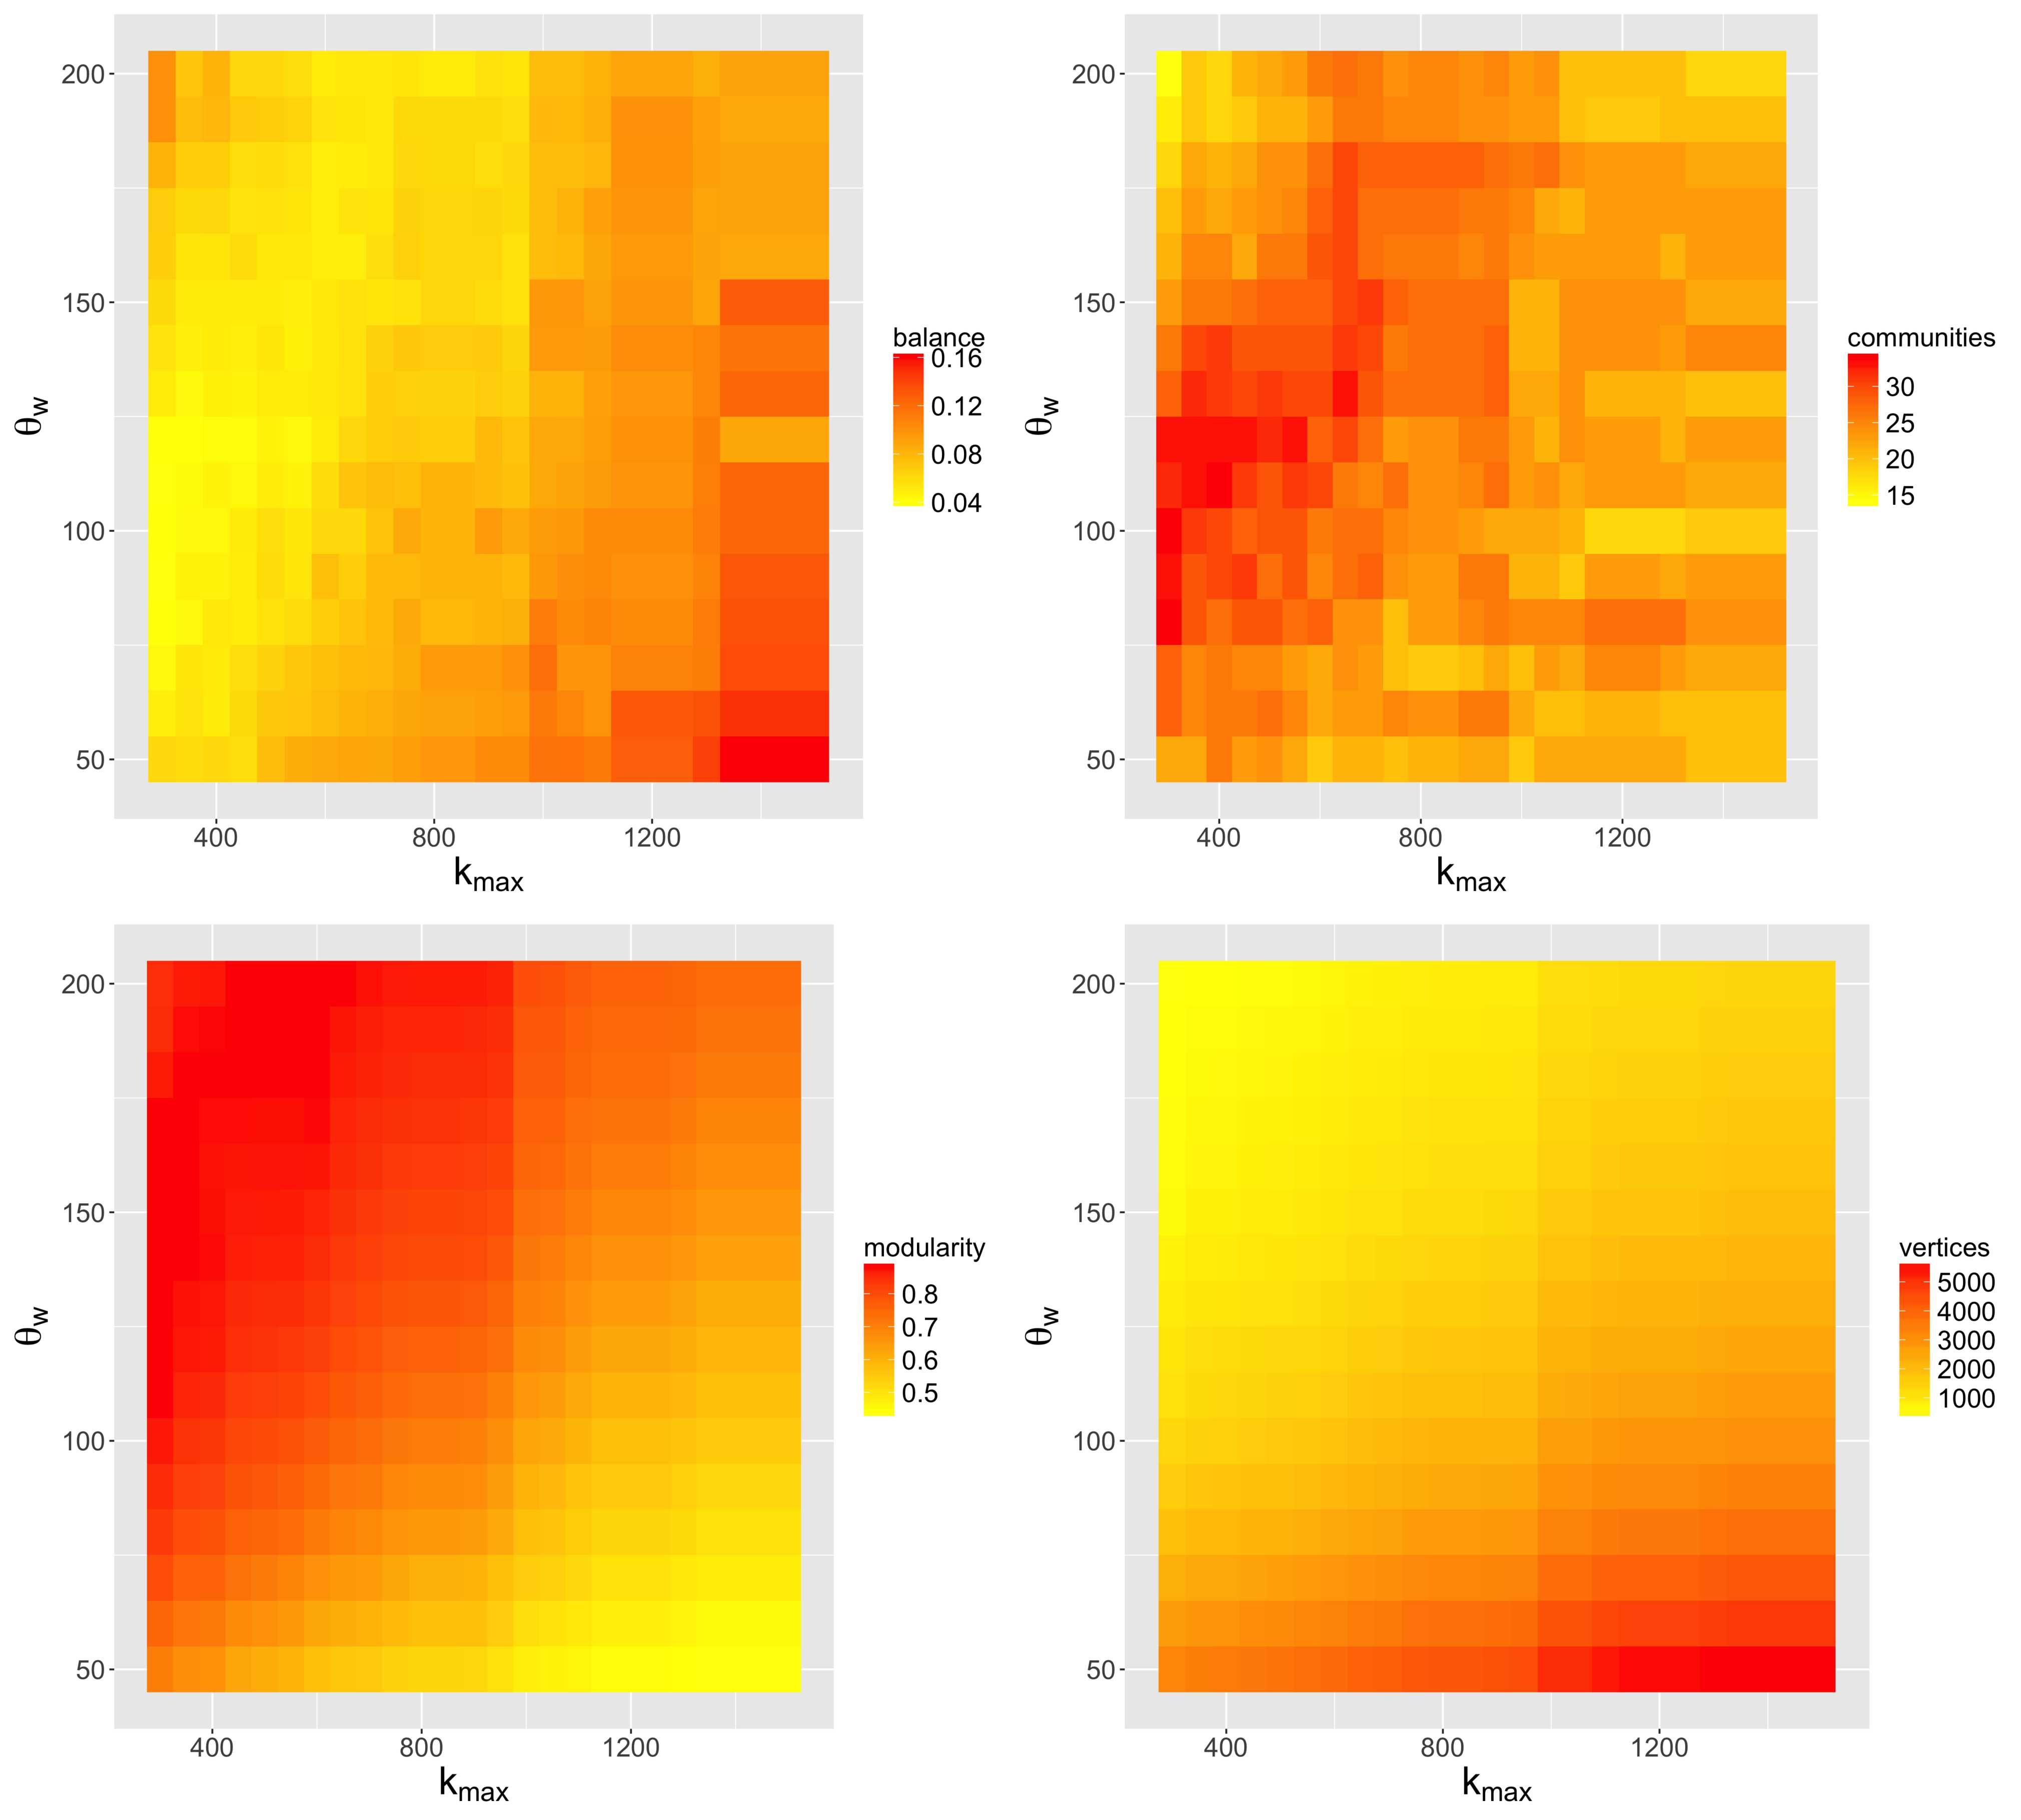
\includegraphics[width=\textwidth]{Figures/Cybergeo/Fig6.jpg}
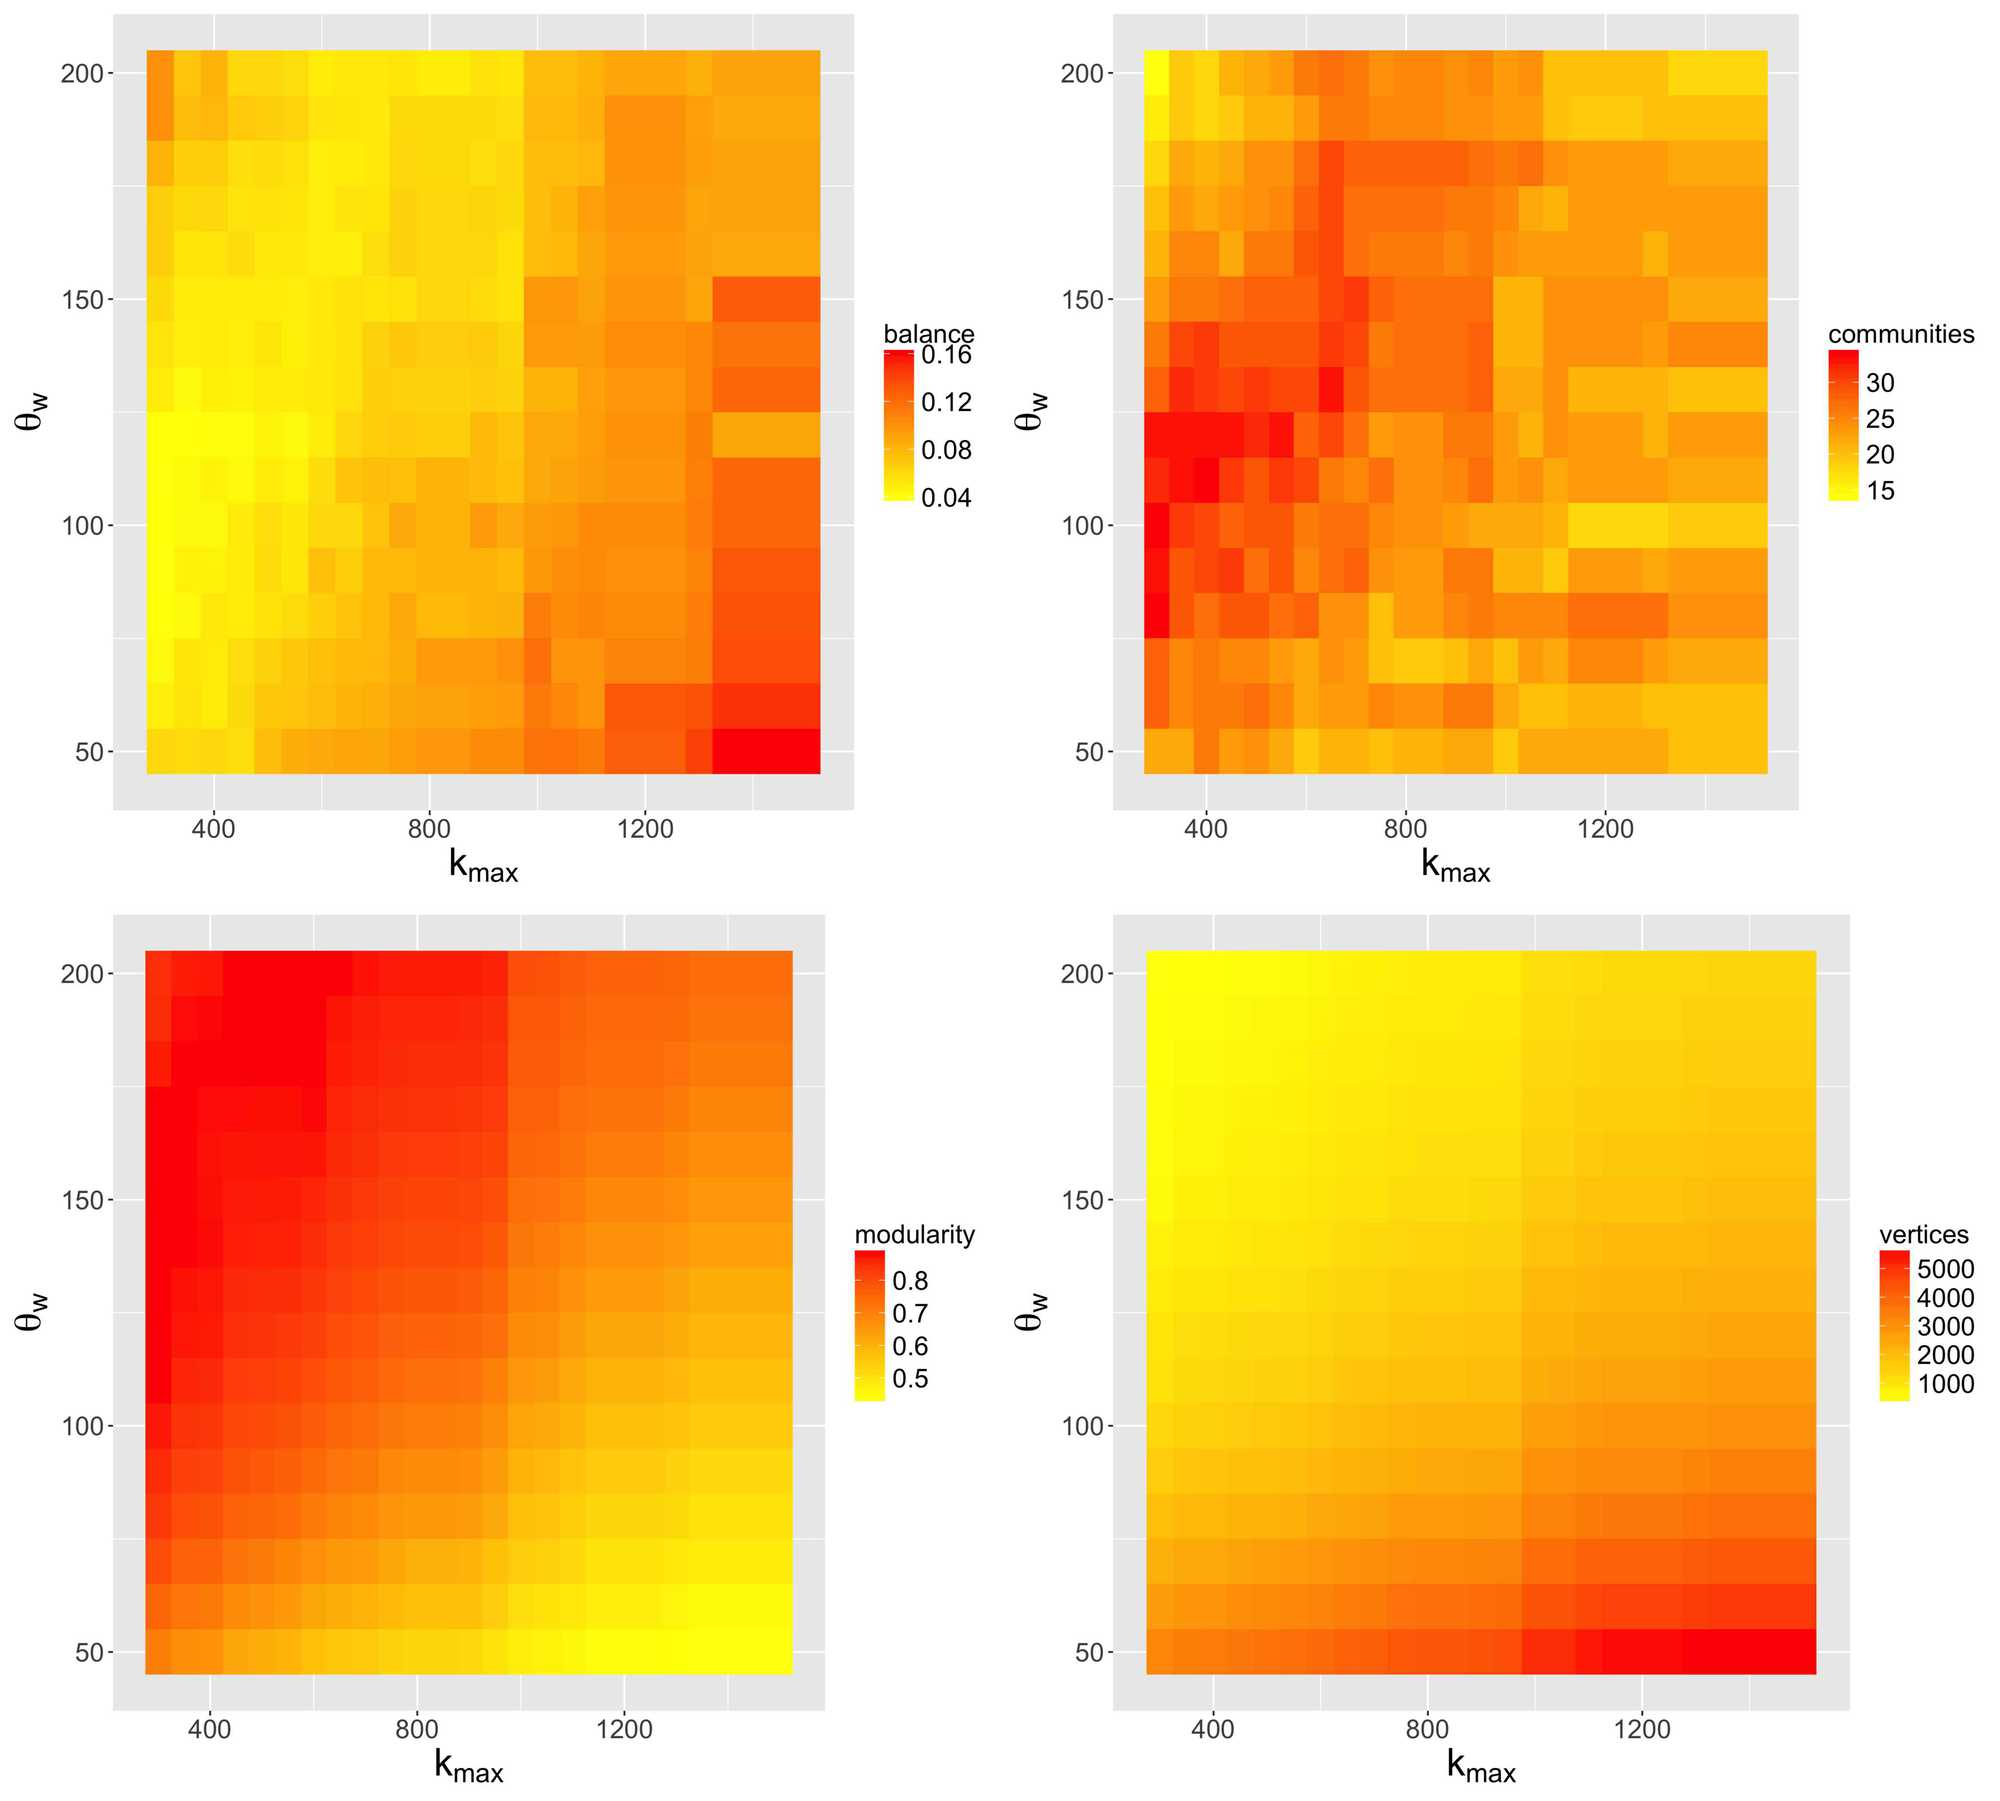
\includegraphics[width=\linewidth]{Figures/Final/B-cybergeo-fig6.jpg}
\appcaption{\textbf{Sensitivity analysis of network indicators to filtering parameters.} We show here 4 indicators (balance between community sizes, modularity of the decomposition, number of communities, number of vertices), as a function of parameters $k_{max}$ and $\theta_w$, at fixed $f_{min} = 50, f_{max} = 10000$. Close values for these two last parameters (in a reasonable range) give similar behavior.\label{fig:cybergeo:fig6}}{\textbf{Analyse de sensibilité des indicateurs de réseau aux paramètres de filtrage.} Nous donnons ici 4 indicateurs (équilibre entre les tailles des communautés, modularité de la décomposition, nombre de communautés, nombre de noeuds), comme fonction des paramètres $k_{max}$ et $\theta_w$, à des valeurs fixées $f_{min} = 50, f_{max} = 10000$. Des valeurs proches pour ces deux derniers paramètres (dans des bornes raisonnables) donne un comportement similaire.\label{fig:cybergeo:fig6}}
\end{figure}
%%%%%%%%%%%%%%%%%%





%%%%%%%%%%%%%%%%%%
\paragraph{Semantic Communities}{Communautés sémantiques}

\bpar{
We obtain therein communities in the semantic network with the optimized filtering parameters. At the exception of a small proportion apparently resulting from noise (representing less than 10 keywords in 3 communities that we remove, i.e. 0.33\% of keywords), communities correspond to well-defined scientific fields, domains, or approaches. Naming is also done by inspection of the most relevant keywords in each community, in order to stick here to a certain level of supervision.
}{
Nous obtenons ainsi des communautés dans le réseau sémantique avec les paramètres de filtration optimisés. A l'exception d'une petite proportion s'apparentant apparemment à du bruit (représentant moins de 10 mots-clés dans 3 communautés que nous supprimons, i.e. 0.33\% des mots-clés), les communautés correspondent à des champ scientifiques, domaines, ou approches bien définis. La dénomination est également faite par inspection des mots-clés les plus pertinents dans chaque communauté, afin de se tenir ici à un certain niveau de supervision.
}

%%%%%%%%%%%%%%%%%%
\begin{table}
\appcaption{\textbf{Semantic communities reconstructed from community detection in the semantic network.}\label{tab:cybergeo:domains}}{\textbf{Composition des communautés sémantiques.} Elles sont construites par détection de communautés dans le réseau sémantique.\label{tab:cybergeo:domains}}
\hspace{-1cm}
\begin{tabular}{lll}
\hline\noalign{\smallskip}
Name & Size & Keywords  \\
\noalign{\smallskip}\hline\noalign{\smallskip}
Political sciences/critical geography & 535 & \texttt{decision-mak, polit ideolog, democraci, stakehold}\\%, neoliber} \\
Biogeography & 394 & \texttt{plant densiti, wood, wetland, riparian veget} \\
Economic geography & 343 &  \texttt{popul growth, transact cost, socio-econom, household}\\%, household incom} \\
Environnment/climate & 309 & \texttt{ice sheet, stratospher, air pollut, climat model} \\
Complex systems & 283 & \texttt{scale-fre, multifract, agent-bas model, self-organ} \\
Physical geography & 203 & \texttt{sedimentari, digit elev model, geolog, river delta} \\
Spatial analysis & 175 & \texttt{spatial analysi, princip compon analysi, heteroscedast}\\%, factor analysi} \\
Microbiology & 118 & \texttt{chromosom, phylogenet, borrelia} \\
Statistical methods & 88 & \texttt{logist regress, classifi, kalman filter, sampl size} \\
Cognitive sciences & 81 & \texttt{semant memori, retrospect, neuroimag} \\
GIS & 75 & \texttt{geograph inform scienc, softwar design, volunt gi}\\%volunt geograph inform, spatial decis support} \\
Traffic modeling & 63 & \texttt{simul model, lane chang, traffic flow, crowd behavior} \\
Health & 52 & \texttt{epidem, vaccin strategi, acut respiratori syndrom}\\%, hospit} \\
Remote sensing & 48 & \texttt{land-cov, landsat imag, lulc} \\
Crime & 17 & \texttt{crimin justic system, social disorgan, crime} \\
\noalign{\smallskip}\hline
\end{tabular}
\end{table}
%%%%%%%%%%%%%%%%%%


%%%%%%%%%%%%%%%%%%
\begin{figure}
%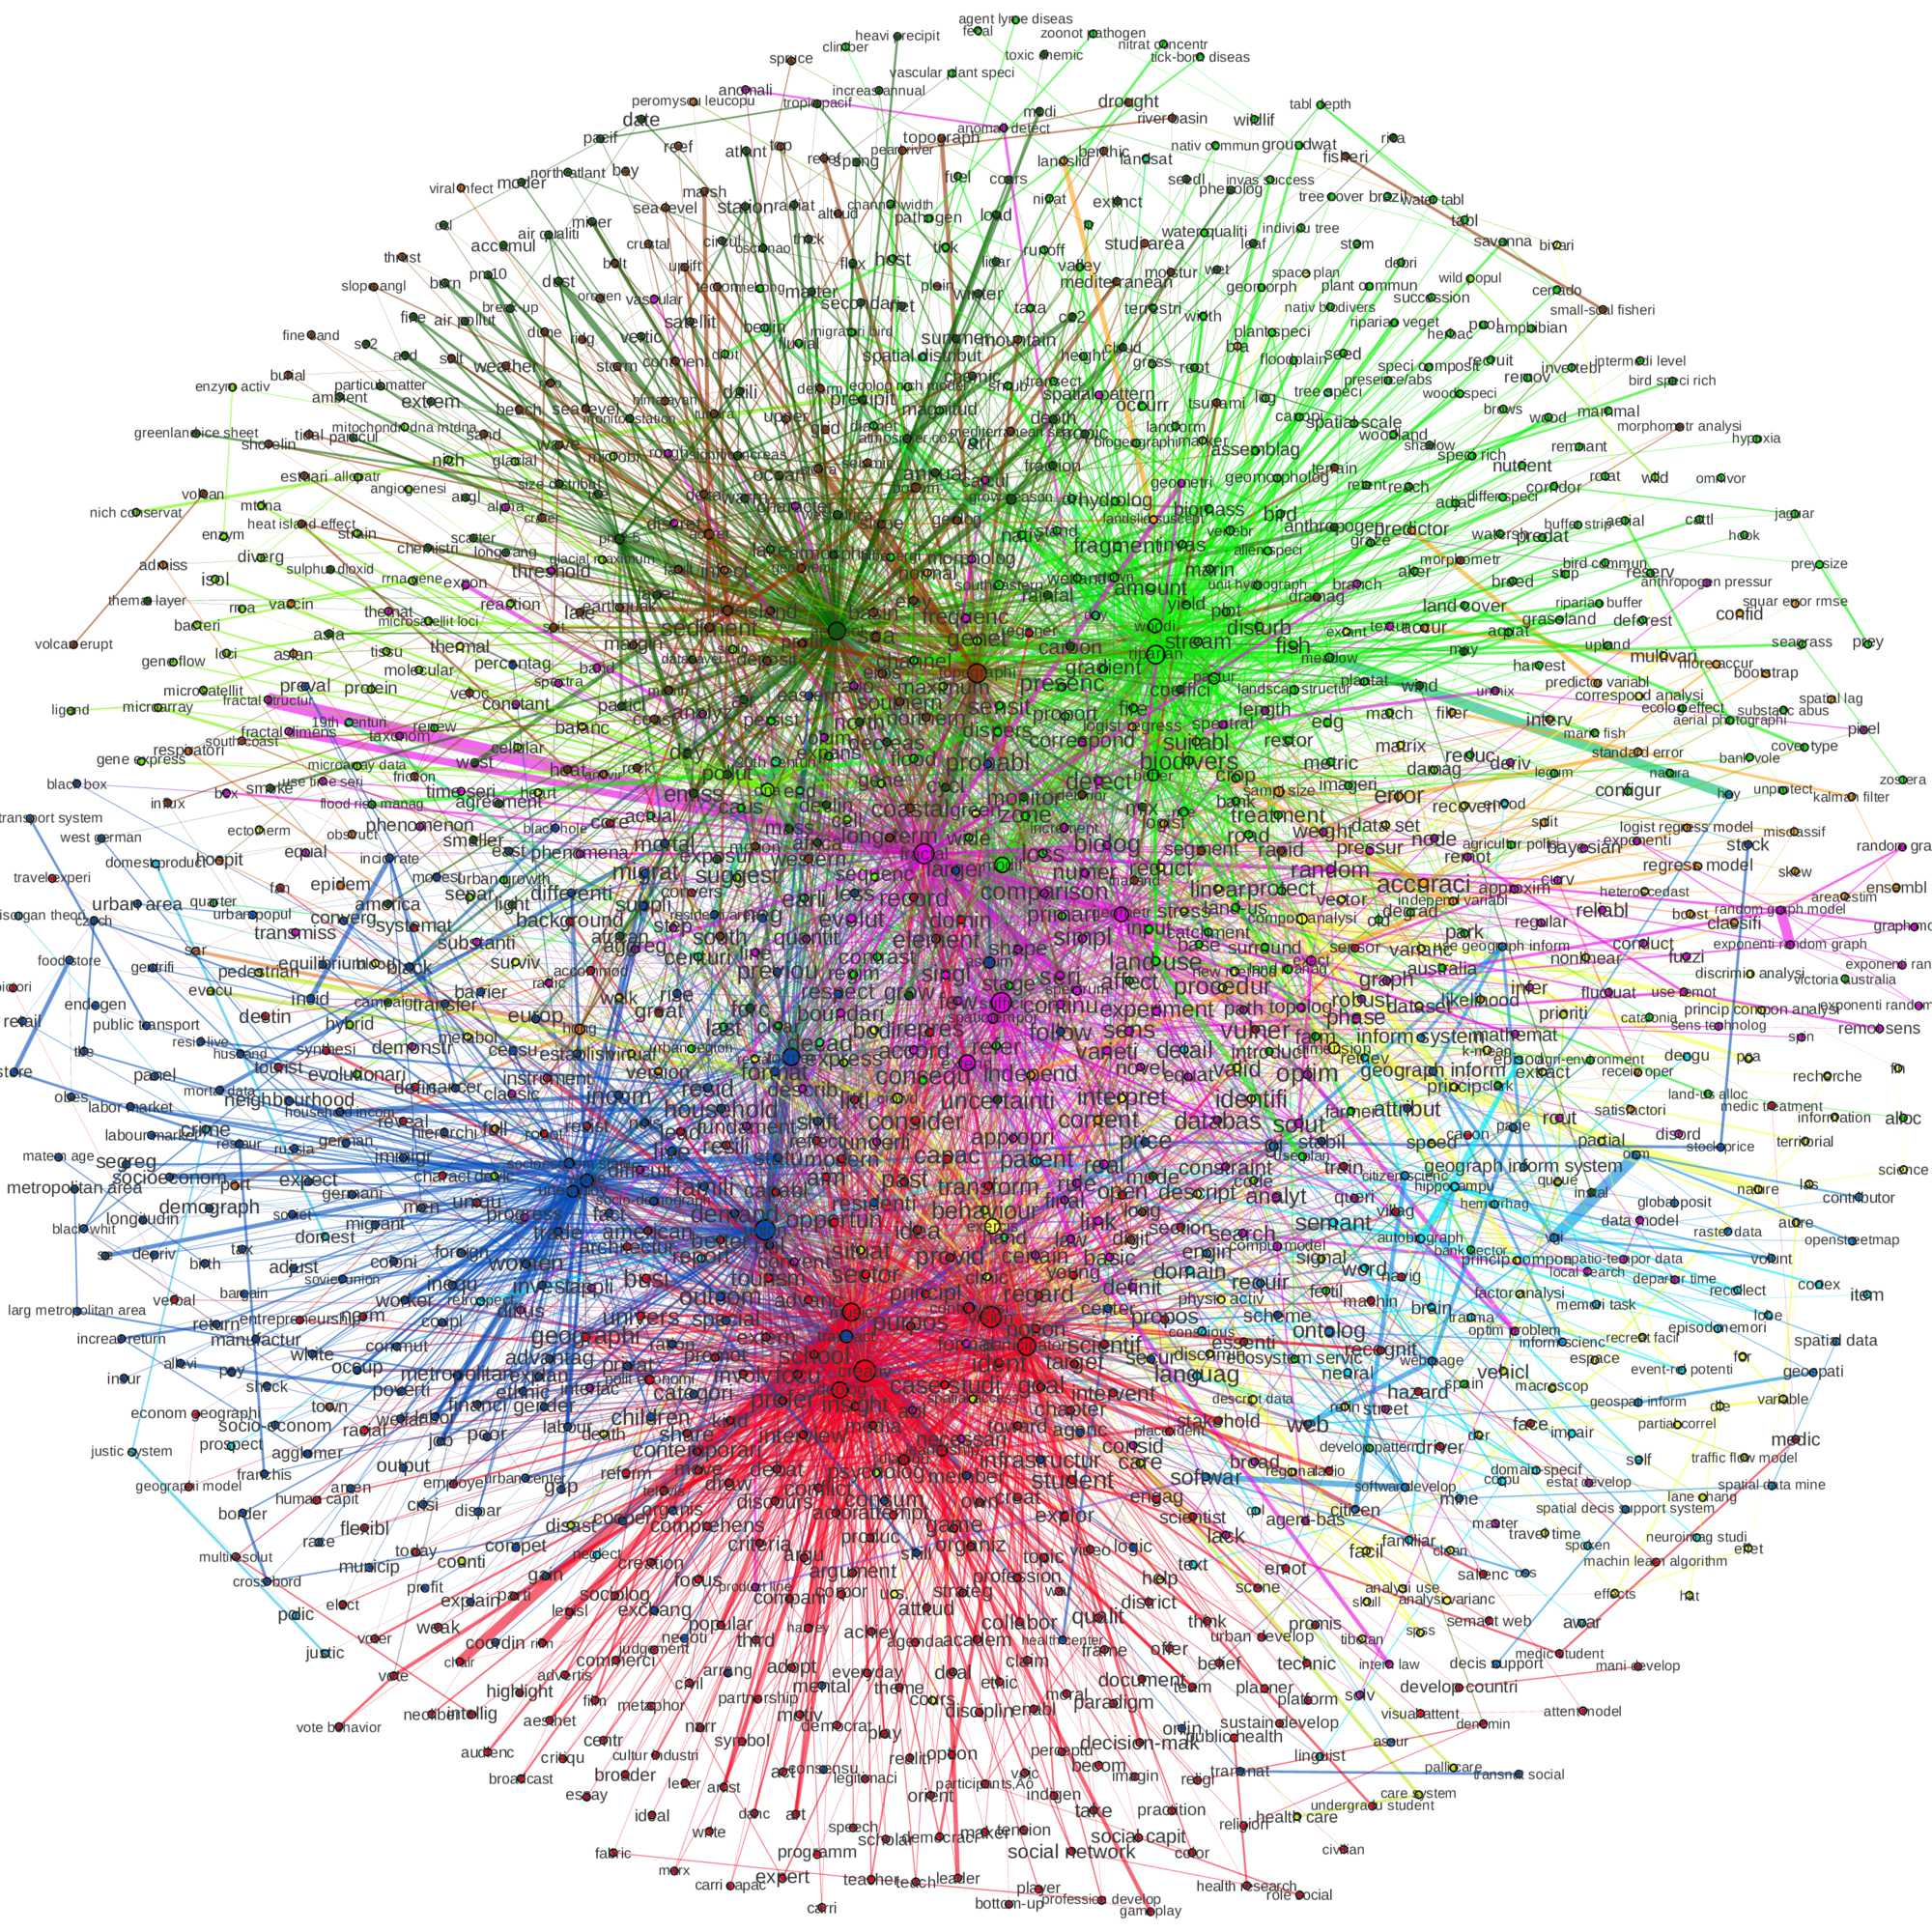
\includegraphics[width=1.6\textwidth]{Figures/Cybergeo/Fig7.jpg}
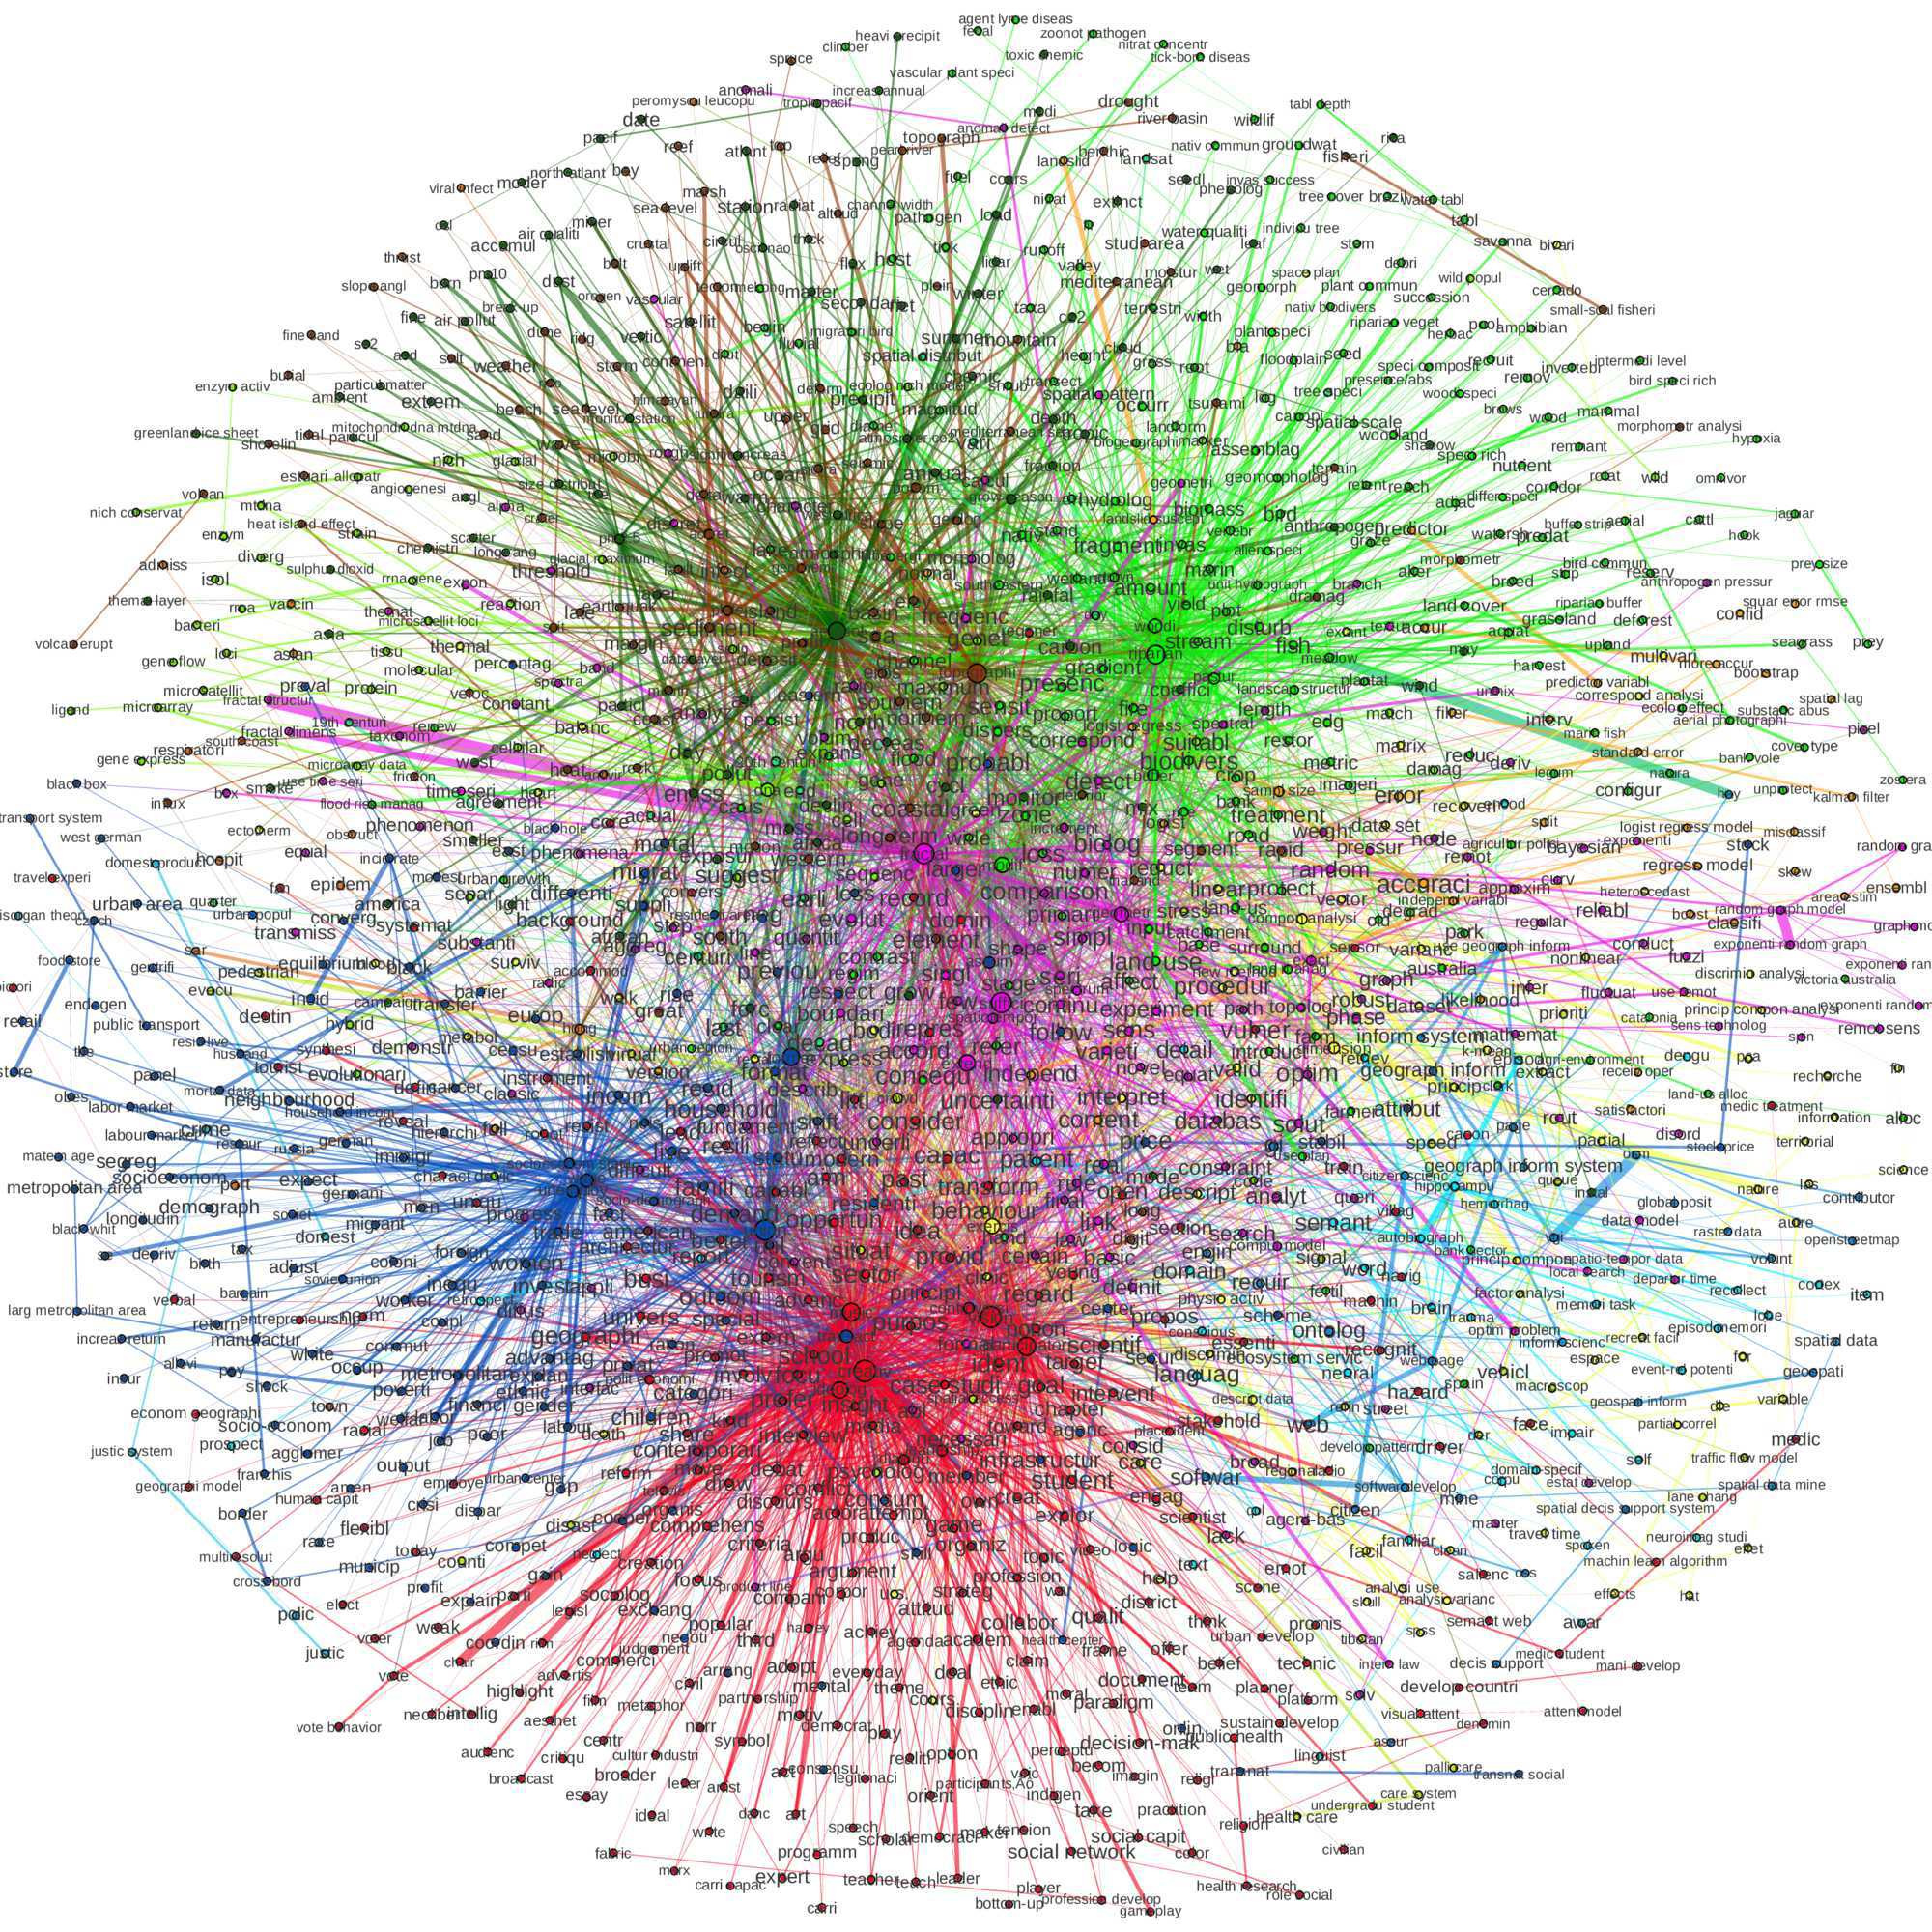
\includegraphics[width=\linewidth]{Figures/Final/B-cybergeo-fig7.jpg}
\appcaption{\textbf{Visualization of the semantic network.} Network is constructed by co-occurrences of most relevant keywords. Filtering parameters are here taken according to the multi-objective optimization done in Fig.~\ref{fig:cybergeo:fig6}, i.e. $(k_{max}=1200,\theta_w=100,f_{min}=50,f_{max}=10000)$. The graph spatialization algorithm (Fruchterman-Reingold), despite its stochastic and path-dependent character, unveils information on the relative positioning of communities.\label{fig:cybergeo:fig7}}{\textbf{Visualisation du réseau sémantique.} Le réseau est construit par co-occurrences des mots-clés les plus pertinents. Les paramètres de filtrage sont pris ici selon l'optimisation multi-objectifs faite en Fig.~\ref{fig:cybergeo:fig6}, i.e. $(k_{max}=1200,\theta_w=100,f_{min}=50,f_{max}=10000)$. L'algorithme de spatialisation du graphe (Fruchterman-Reingold), malgré son caractère stochastique et dépendant au chemin, révèle de l'information sur le positionnement relatif des communautés.\label{fig:cybergeo:fig7}}
\end{figure}
%%%%%%%%%%%%%%%%%%



%%%%%%%%%%%%%%%%%%
\begin{figure}
%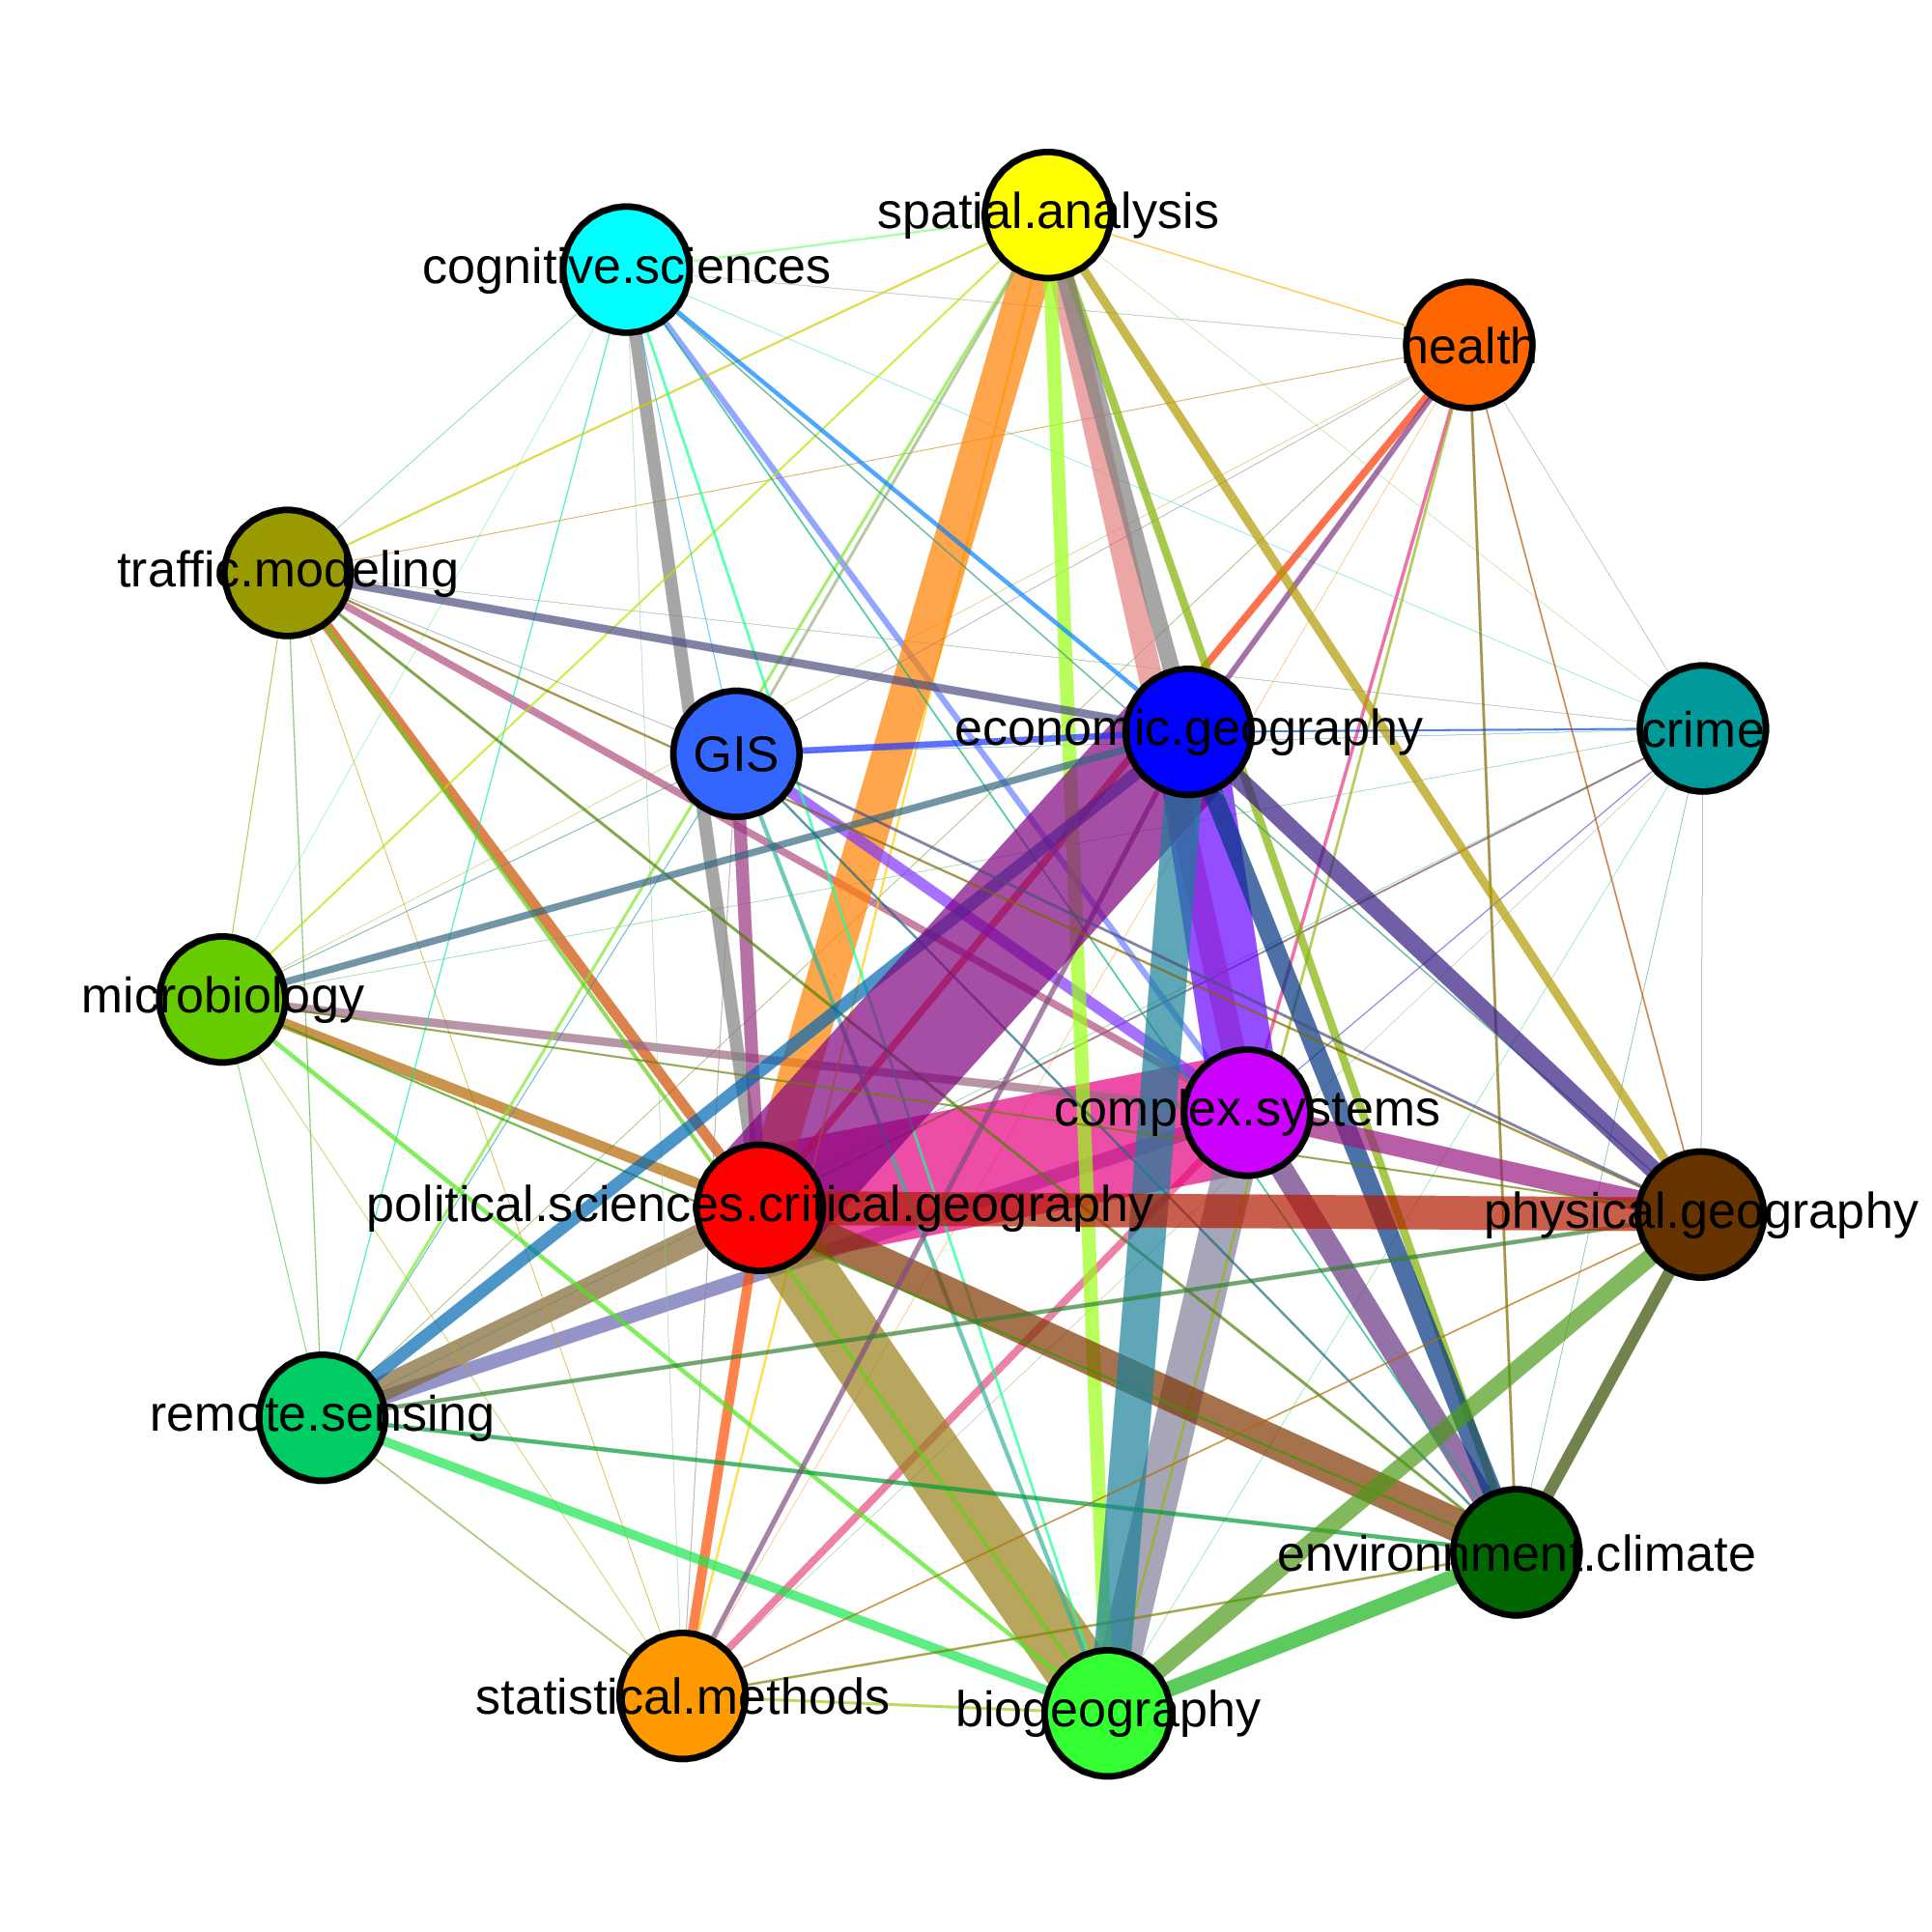
\includegraphics[width=\textwidth]{Figures/Cybergeo/Fig8.jpg}
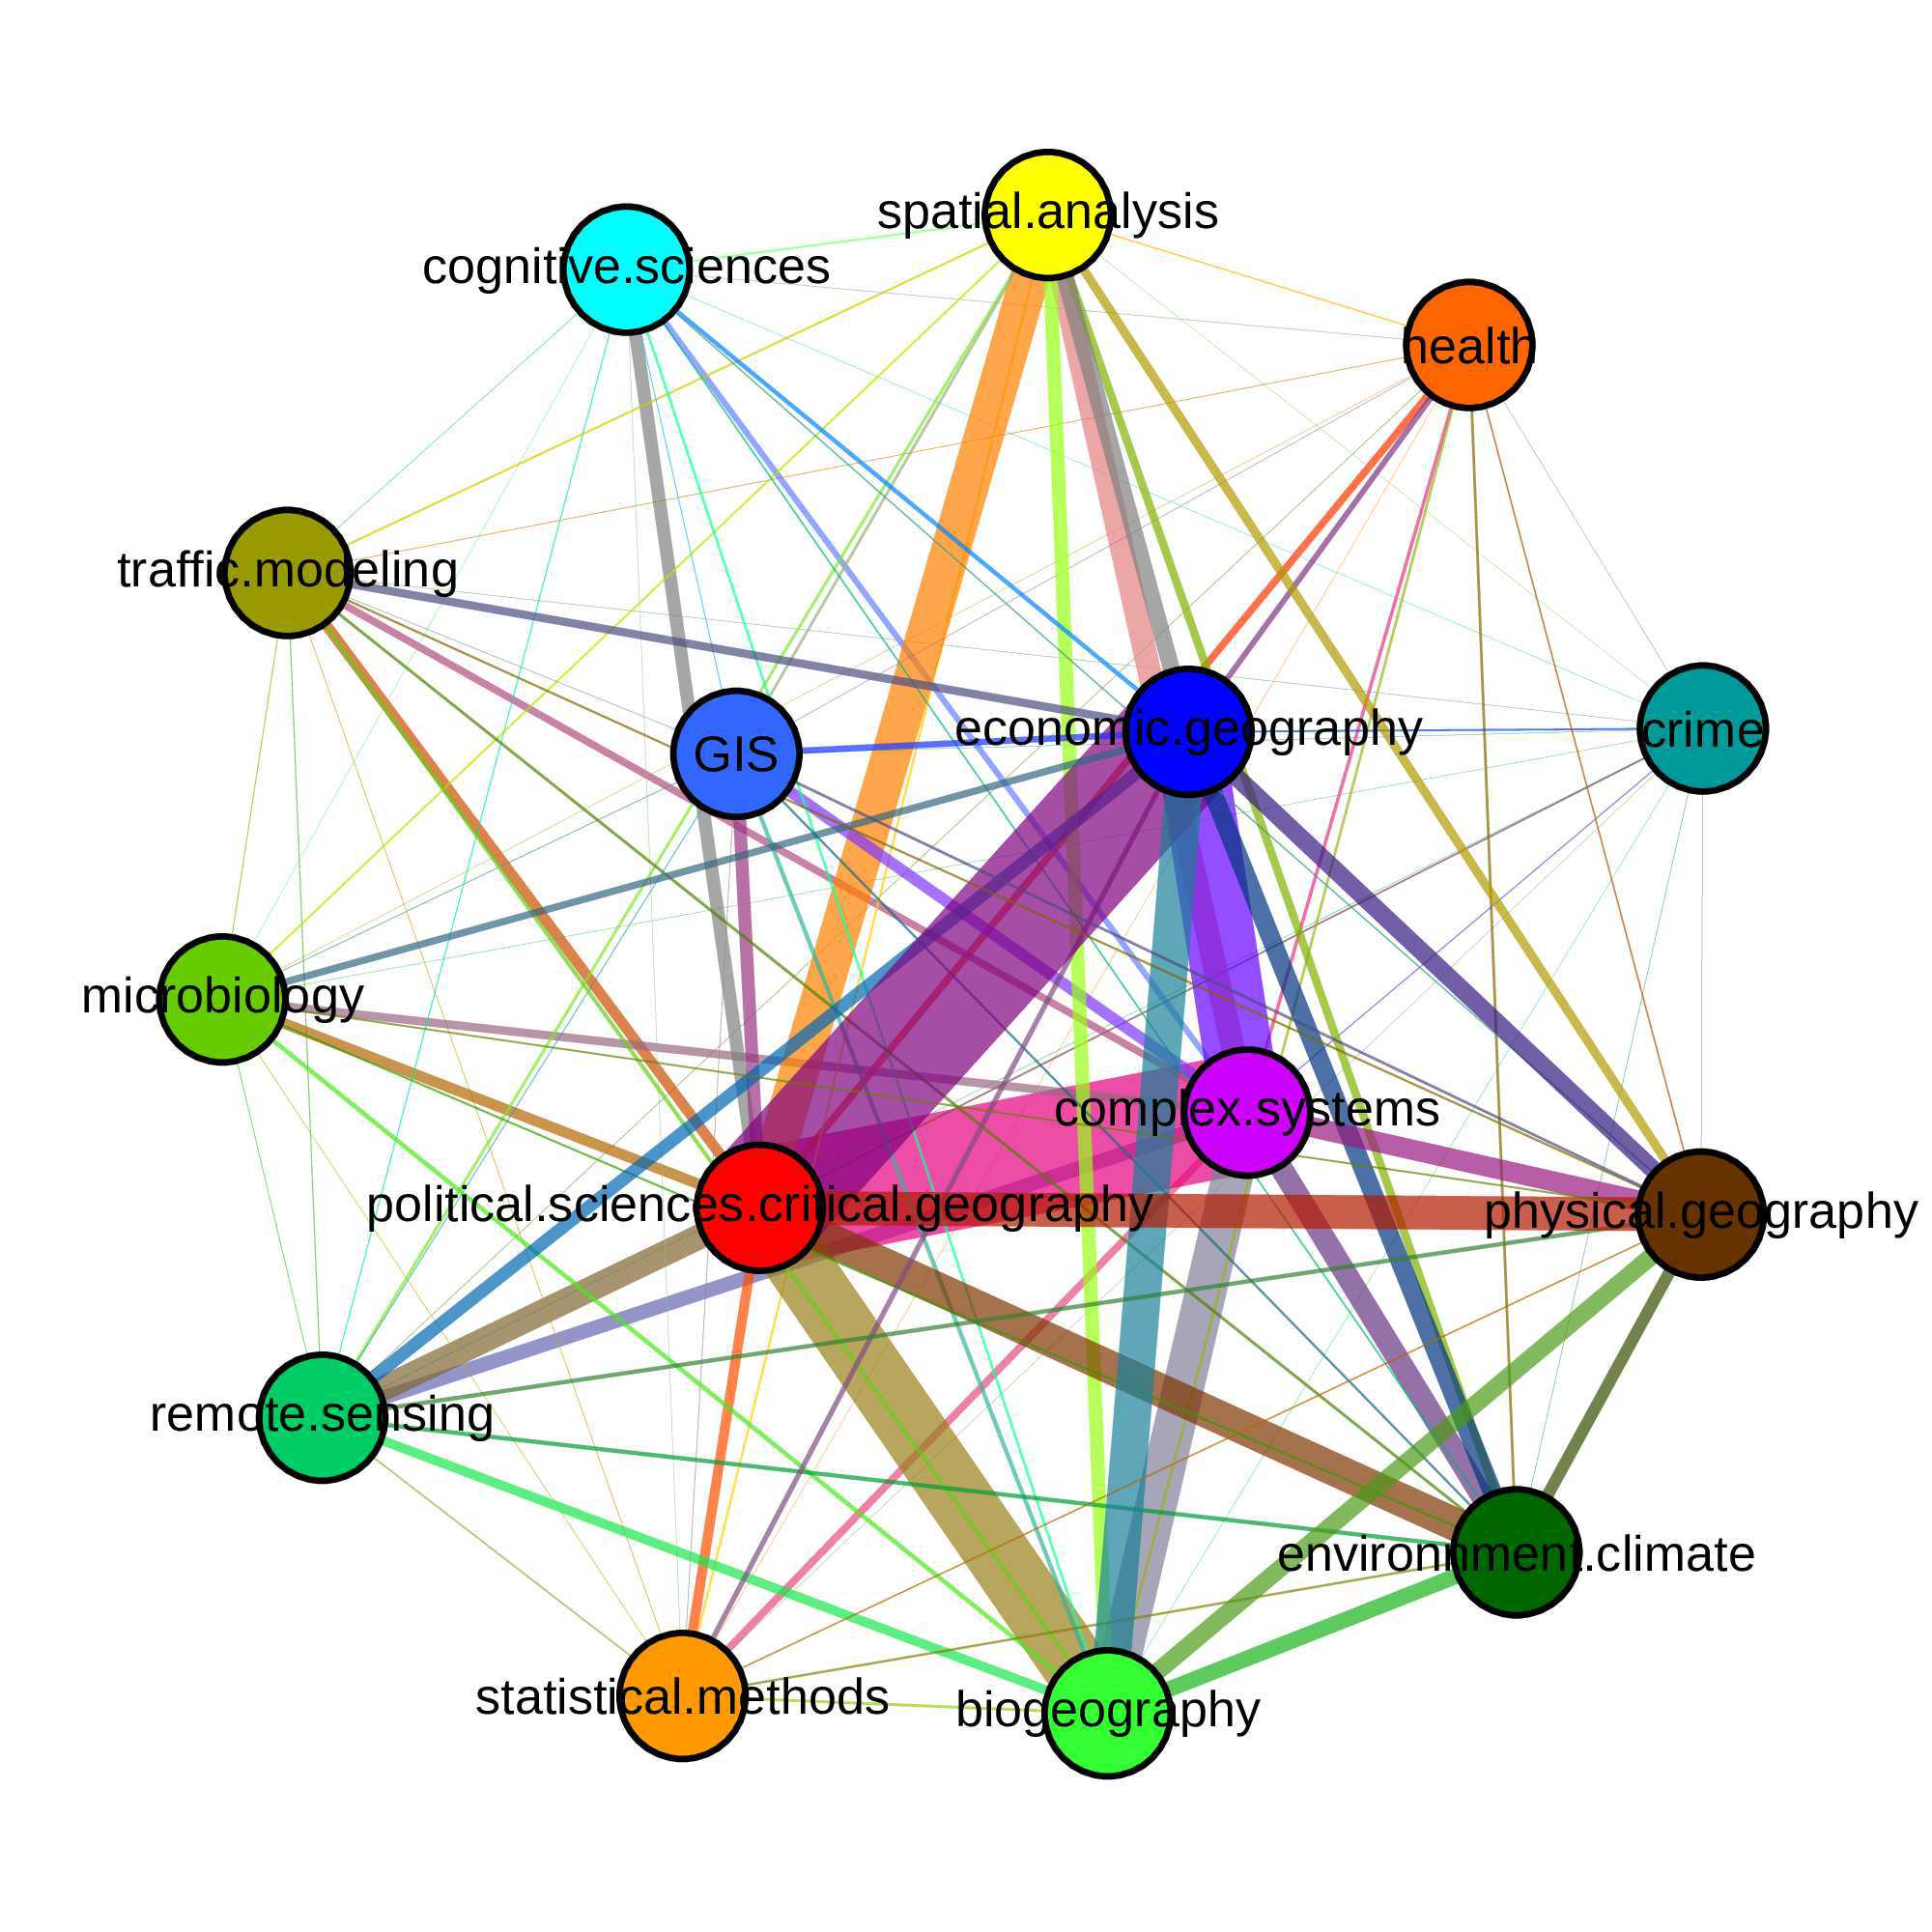
\includegraphics[width=\linewidth]{Figures/Final/B-cybergeo-fig8.jpg}
\appcaption{\textbf{Synthesis of semantic communities and their links.} Weights of links are computed as probabilities of co-occurrences of corresponding keywords within references.\label{fig:cybergeo:fig8}}{\textbf{Synthèse des communautés sémantiques et de leurs liens.} Les poids des liens sont calculés comme les probabilités de co-occurrence des mots-clés correspondants au sein des références.\label{fig:cybergeo:fig8}}
\end{figure}
%%%%%%%%%%%%%%%%%%


\bpar{
Table~\ref{tab:cybergeo:domains} summarizes the communities, giving their names, sizes, and corresponding keywords. The most important community is related to issues in political science and critical geography, what could have been expected as several previously obtained citations communities (Social geography, Urban studies) deal with these issues. We then obtain a large cluster of terms related to biogeography, that must correspond to publications in Ecology and Socio-ecology identified before, together with a community in Environment and Climate.
}{
La Table~\ref{tab:cybergeo:domains} résume les communautés, donnant leurs noms, tailles, et mots-clés correspondants. La communauté la plus importante est en rapport avec des questions de Sciences politiques et de Géographie critique, ce qui pouvait être attendu puisque plusieurs communautés de citation obtenues précédemment (\textit{Social Geography}, \textit{Urban Studies}) s'occupent de ces questions. Nous obtenons ensuite un groupement conséquent en termes de biogéographie, qui doit correspondre aux publications en écologie et socio-écologie identifiées précédemment, avec une communauté en environnement et climat.
}


\bpar{
In a way similar to the citation communities, but more pronounced here, we obtain endogenous ``disciplines'' that can correspond to real disciplines, to methodologies, to object of studies. This classification thus also unveil \emph{effective scientific practices}, here in terms of semantic content. A class here related to complex systems can be associated to a paradigm and various approaches that were separated in the citation communities : agent-based models and complex networks for example. On the contrary, some studies that were gathered in a large domain before can be precisely differentiated in the semantic network, such as microbiology and health here that are used by studies related to socio-ecology or ecology in the citation network. Some very specific domains appear here as they have very few connections in their actual semantic content : for example, Geography of crime is very precise and disconnected from other communities.
}{
De manière similaire au communautés de citation, mais plus prononcée ici, nous obtenons des ``disciplines'' endogènes qui peuvent correspondre à des vraies disciplines, à des méthodologies, à des objets d'étude. Cette classification révèle pour cela également des \emph{pratiques scientifiques effectives}, ici en termes de contenu sémantique. Une classe ici en rapport avec les Systèmes Complexes peut être associées à un paradigme et à différentes approches qui étaient séparées dans les communautés de citation : les modèles basés-agent et les réseaux complexes par exemple. Au contraire, certaines études qui étaient rassemblées dans de larges domaines précédemment peuvent être différenciées précisément dans le réseau sémantique, comme la microbiologie et la santé ici qui sont utilisées par des études en relation à l'écologie et la socio-écologie dans le réseau de citation. Certains domaines très spécifiques apparaissent ici puisqu'ils ont très peu de connections avec les autres dans leur contenu sémantique : par exemple, la géographie du crime est très précise et déconnectée des autres communautés.
}


\bpar{
We show in Fig.~\ref{fig:cybergeo:fig7} a visualisation of the semantic network, in which the positioning of communities, induced by a Fruchterman-Reingold algorithm (that we use here to have a more precise layout in the relative positioning compared to Force Atlas~\citep{jacomy2014forceatlas2}). The bridging between distant disciplines is done quite differently compared to the citation network, and reveals thus qualitatively an other dimension of interdisciplinarity, i.e. the semantics shared by disciplines. Here, the communities corresponding to Economic Geography (blue) and to Critical Geography (red) are close as in the citation network, but are linked to ecology and geomorphology (green and brown) by Complex Systems (magenta), although these were not present as a community in the citation network. Complexity methodologies such as Fractals, Scaling~\citep{west2017scale} or Networks~\citep{newman2003structure} are indeed widely used both in social sciences and in physics or biology. The semantic analysis reveals thus that very distant disciplines, that are distant in their citation patterns, are finally close in terms of actual content.
}{
Nous montrons en Fig.~\ref{fig:cybergeo:fig7} une visualisation du réseau sémantique, dans lequel le positionnement des communautés, induit par un algorithme de Fruchterman-Reingold (que nous utilisons ici pour avoir un positionnement plus précis dans le positionnement relatif en comparaison du Force-Atlas~\citep{jacomy2014forceatlas2}). Les ponts entre disciplines distantes est effectué différemment en comparaison du réseau de citation, et révèle ainsi qualitativement une autre dimension de l'interdisciplinarité, i.e. la sémantique partagée par les disciplines. Ici, les communautés correspondant à l'Economie Géographique (bleu) et à la Géographie critique (rouge) sont proches dans le réseau de citation, mais sont liés à l'écologie et la géomorphologie (vert et marron) par les Systèmes Complexes (magenta), bien que ceux-ci n'étaient pas présents comme communauté dans le réseau de citation. Les méthodologies de la complexité comme les fractales, les loi d'échelles~\cite{west2017scale}, ou les réseaux~\cite{newman2003structure} sont en effet largement utilisés à la fois en sciences sociales et en physique ou biologie. L'analyse sémantique montre ainsi que des disciplines très distantes, qui sont distantes dans leur motifs de citation, sont finalement proches en termes de contenu observé.
}


\bpar{
In terms of overlaps between communities, in the sense of co-occurrences of corresponding keywords within texts of references, we show a synthesis of links between semantic communities in Fig.~\ref{fig:cybergeo:fig8}. We see that communities such as Critical Geography and Biogeography are not totally disconnected and share still a certain number of co-occurrences. More isolated communities can be spotted such as Health and Crime Geographies. Surprisingly, Statistical Methods does not share strong links with other communities, what could mean that articles dealing with methodological issues in this field are rather disconnected from the field of application, or at least do not describe it extensively. On the contrary, methods in Complex Systems are organically integrated with the thematic issues they tackle.
}{
En termes de chevauchements entre les communautés, au sens des co-occurrences des mots-clés correspondants dans les textes des références, nous montrons une synthèse des liens entre communautés sémantiques en Fig.~\ref{fig:cybergeo:fig8}. Nous voyons que les communautés comme la Géographie critique et la biogéographie ne sont pas totalement déconnectées et partagent finalement un certain nombre de co-occurrences. Des communautés plus isolées peuvent être identifiées comme les géographies de la Santé et du Crime. De manière surprenante, les méthodes statistiques ne partagent pas de liens forts avec d'autres communautés, ce qui pourrait signifier que des articles traitant de questions méthodologiques dans ce champ sont plutôt déconnectées du champ d'application, ou au moins ne le décrivent pas en détail. Au contraire, les méthodes en Systèmes Complexes sont organiquement intégrées avec les questions thématiques qu'ils traitent.
}







%%%%%%%%%%%%%%%%%%
\subsubsection{Semantic composition of citation communities}{Composition sémantique des communautés de citation}


%%%%%%%%%%%%%%%%%%
\begin{figure}
%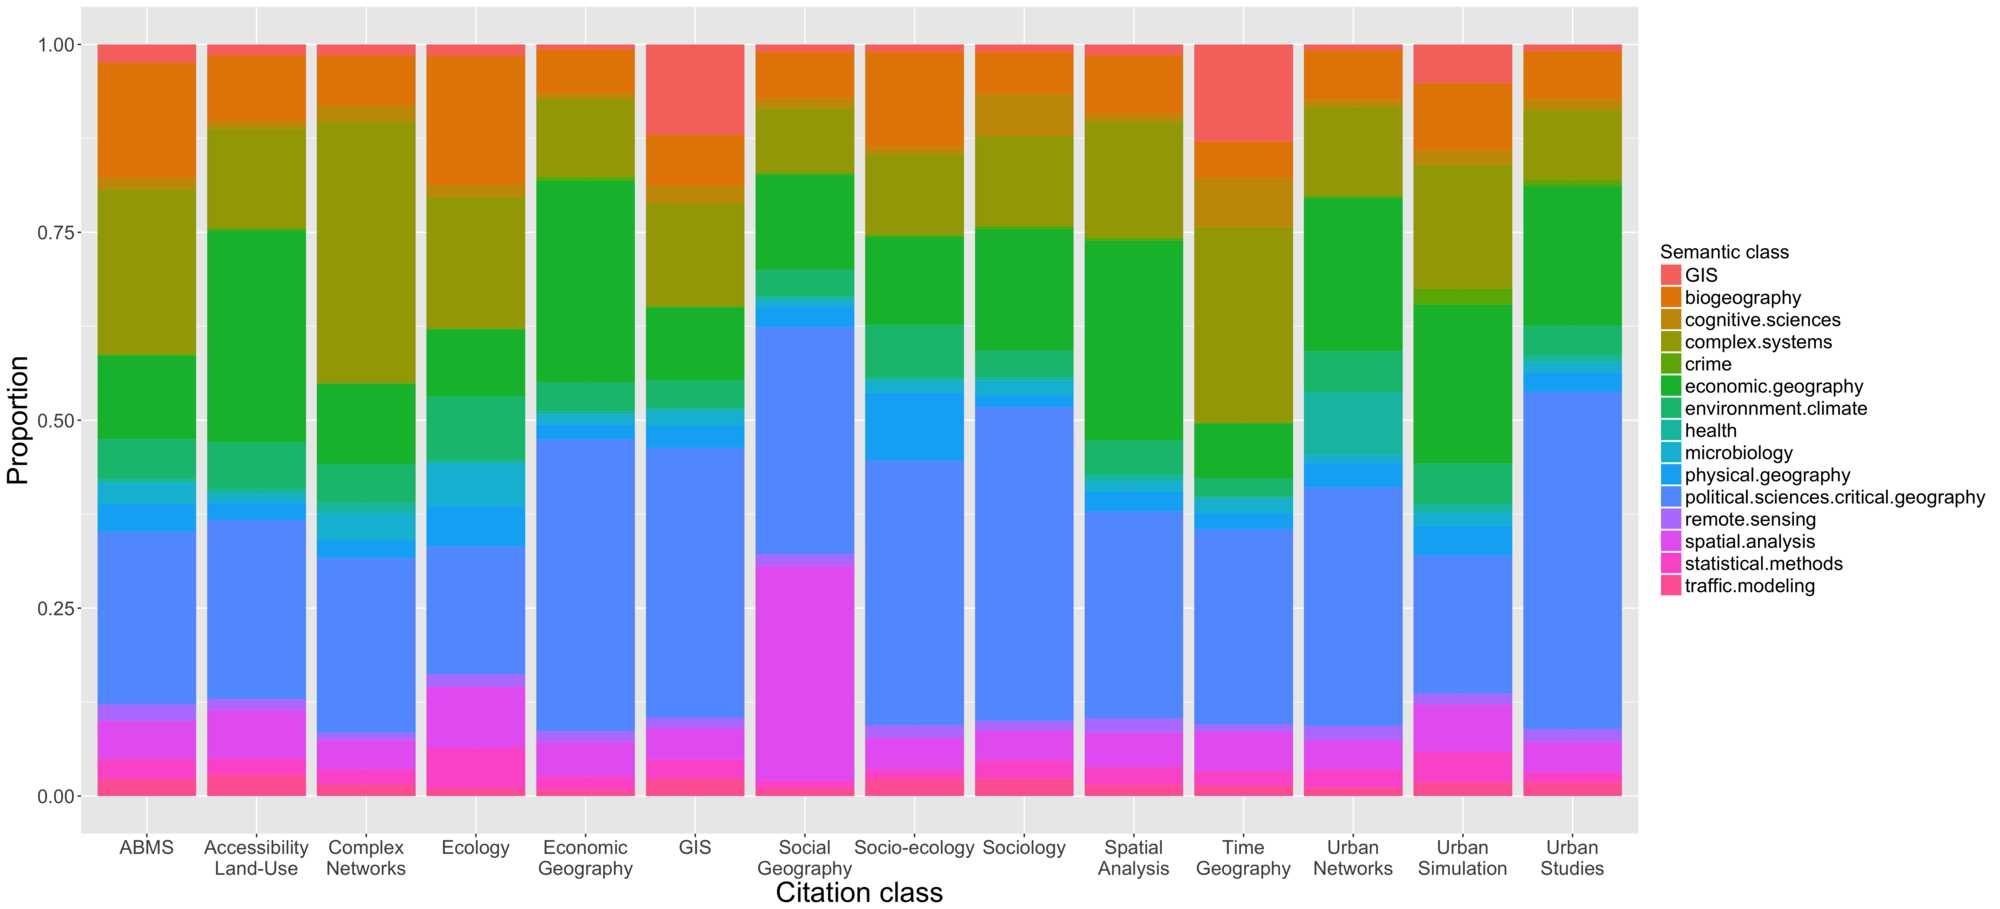
\includegraphics[width=\textwidth]{Figures/Cybergeo/Fig9.jpg}
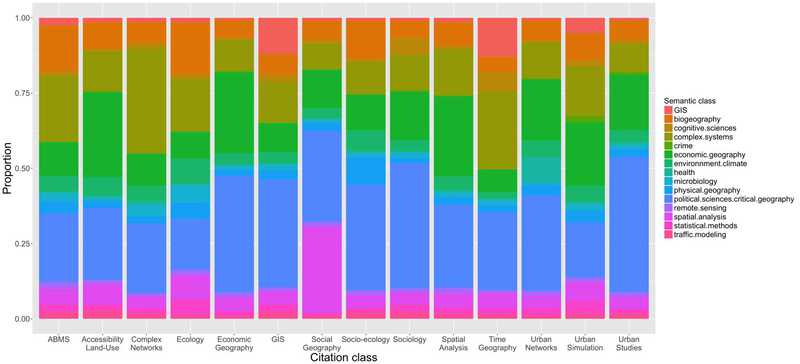
\includegraphics[width=\linewidth]{Figures/Final/B-cybergeo-fig9.jpg}
\appcaption{\textbf{Composition of citation communities in terms of semantic content.} For each citation class (horizontally), the bar is decomposed as the proportions of each semantic class (given by color).\label{fig:cybergeo:fig9}}{\textbf{Composition des communautés de citation en termes de contenu sémantique.} Pour chaque classe de citation (horizontalement), la barre est décomposée entre les proportions de chaque classe sémantique (données par la couleur).\label{fig:cybergeo:fig9}}
\end{figure}
%%%%%%%%%%%%%%%%%%


\bpar{
We can now turn to the study of the relation between classifications. First, a simple way to link them is to look at the semantic content of citation communities. Each reference has a given proportion of keywords within each semantic class, and an average composition in terms of semantic classes for each citation class can thus be computed. We show these composition in Fig.~\ref{fig:cybergeo:fig9}. Some expected results are obtained, such as Complex Networks (citation) having the largest part in Complex Systems (semantic), or GIS (citation) the largest in GIS (semantic), and similarly for Economic Geography.
}{
Nous pouvons à présent nous tourner vers l'étude des relations entre classifications. Tout d'abord, une façon simple de les relier est d'étudier le contenu sémantique des communautés de citations. Chaque référence a une proportion donnée de mots-clés dans chaque classe sémantique, et une composition moyenne en termes de classes sémantiques pour chaque classe de citation peut ainsi être calculée. Nous montrons ces compositions en Fig.~\ref{fig:cybergeo:fig9}. Des résultats attendus sont obtenus, comme \textit{Complex Networks} (citation) ayant la proportion la plus forte en \textit{Complex Systems} (sémantique), ou le GIS (citation) le plus fort en GIS (sémantique), et de même pour l'économie géographique.
}


\bpar{
But the study of patterns that could have not been expected is very informative, and unveils practices of interdisciplinarity. For example, Time Geography (citation) uses as much GIS (semantic) as GIS (citation), what means that they should be using the corresponding methods and tools to study the thematic question of spatio-temporal trajectories of geographical agents. The most important in terms of political science (semantic) are Urban Studies, what suggest a convergence of the City as an object of study and of the disciplines of Political Science and Critical Geography. Also interestingly, the citation communities using most biogeography are Ecology (what could have been expected) and ABMS, confirming again the role of the thematic application in complex systems methodologies.
}{
Mais l'étude de motifs qui auraient pu ne pas être attendus est très informatif, et dévoile des pratiques d'interdisciplinarité. Par exemple, la \textit{Time Geography} (citation) utilise quasiment autant de GIS (sémantique) que le GIS (citation), ce qui signifie qu'ils doivent utiliser les méthodes et outils correspondants pour étudier la question thématique des trajectoires spatio-temporelles des agents géographiques. Le plus important en termes de sciences politiques (sémantique) sont les \textit{Urban Studies}, ce qui suggère une convergence de la Ville comme objet d'étude et des disciplines de Sciences politiques et de Géographie critique. Egalement de manière intéressante, les communautés de citation utilisant le plus la biogéographie sont l'écologie (ce qui pouvait être attendu) et les ABMS, confirmant ainsi le rôle de l'application thématique dans les méthodologies des Systèmes Complexes.
}




%%%%%%%%%%%%%%%%%%
\subsubsection{Measuring interdisciplinarity}{Mesure de l'interdisciplinarité}


%%%%%%%%%%%%%%%%%%
\begin{figure}
%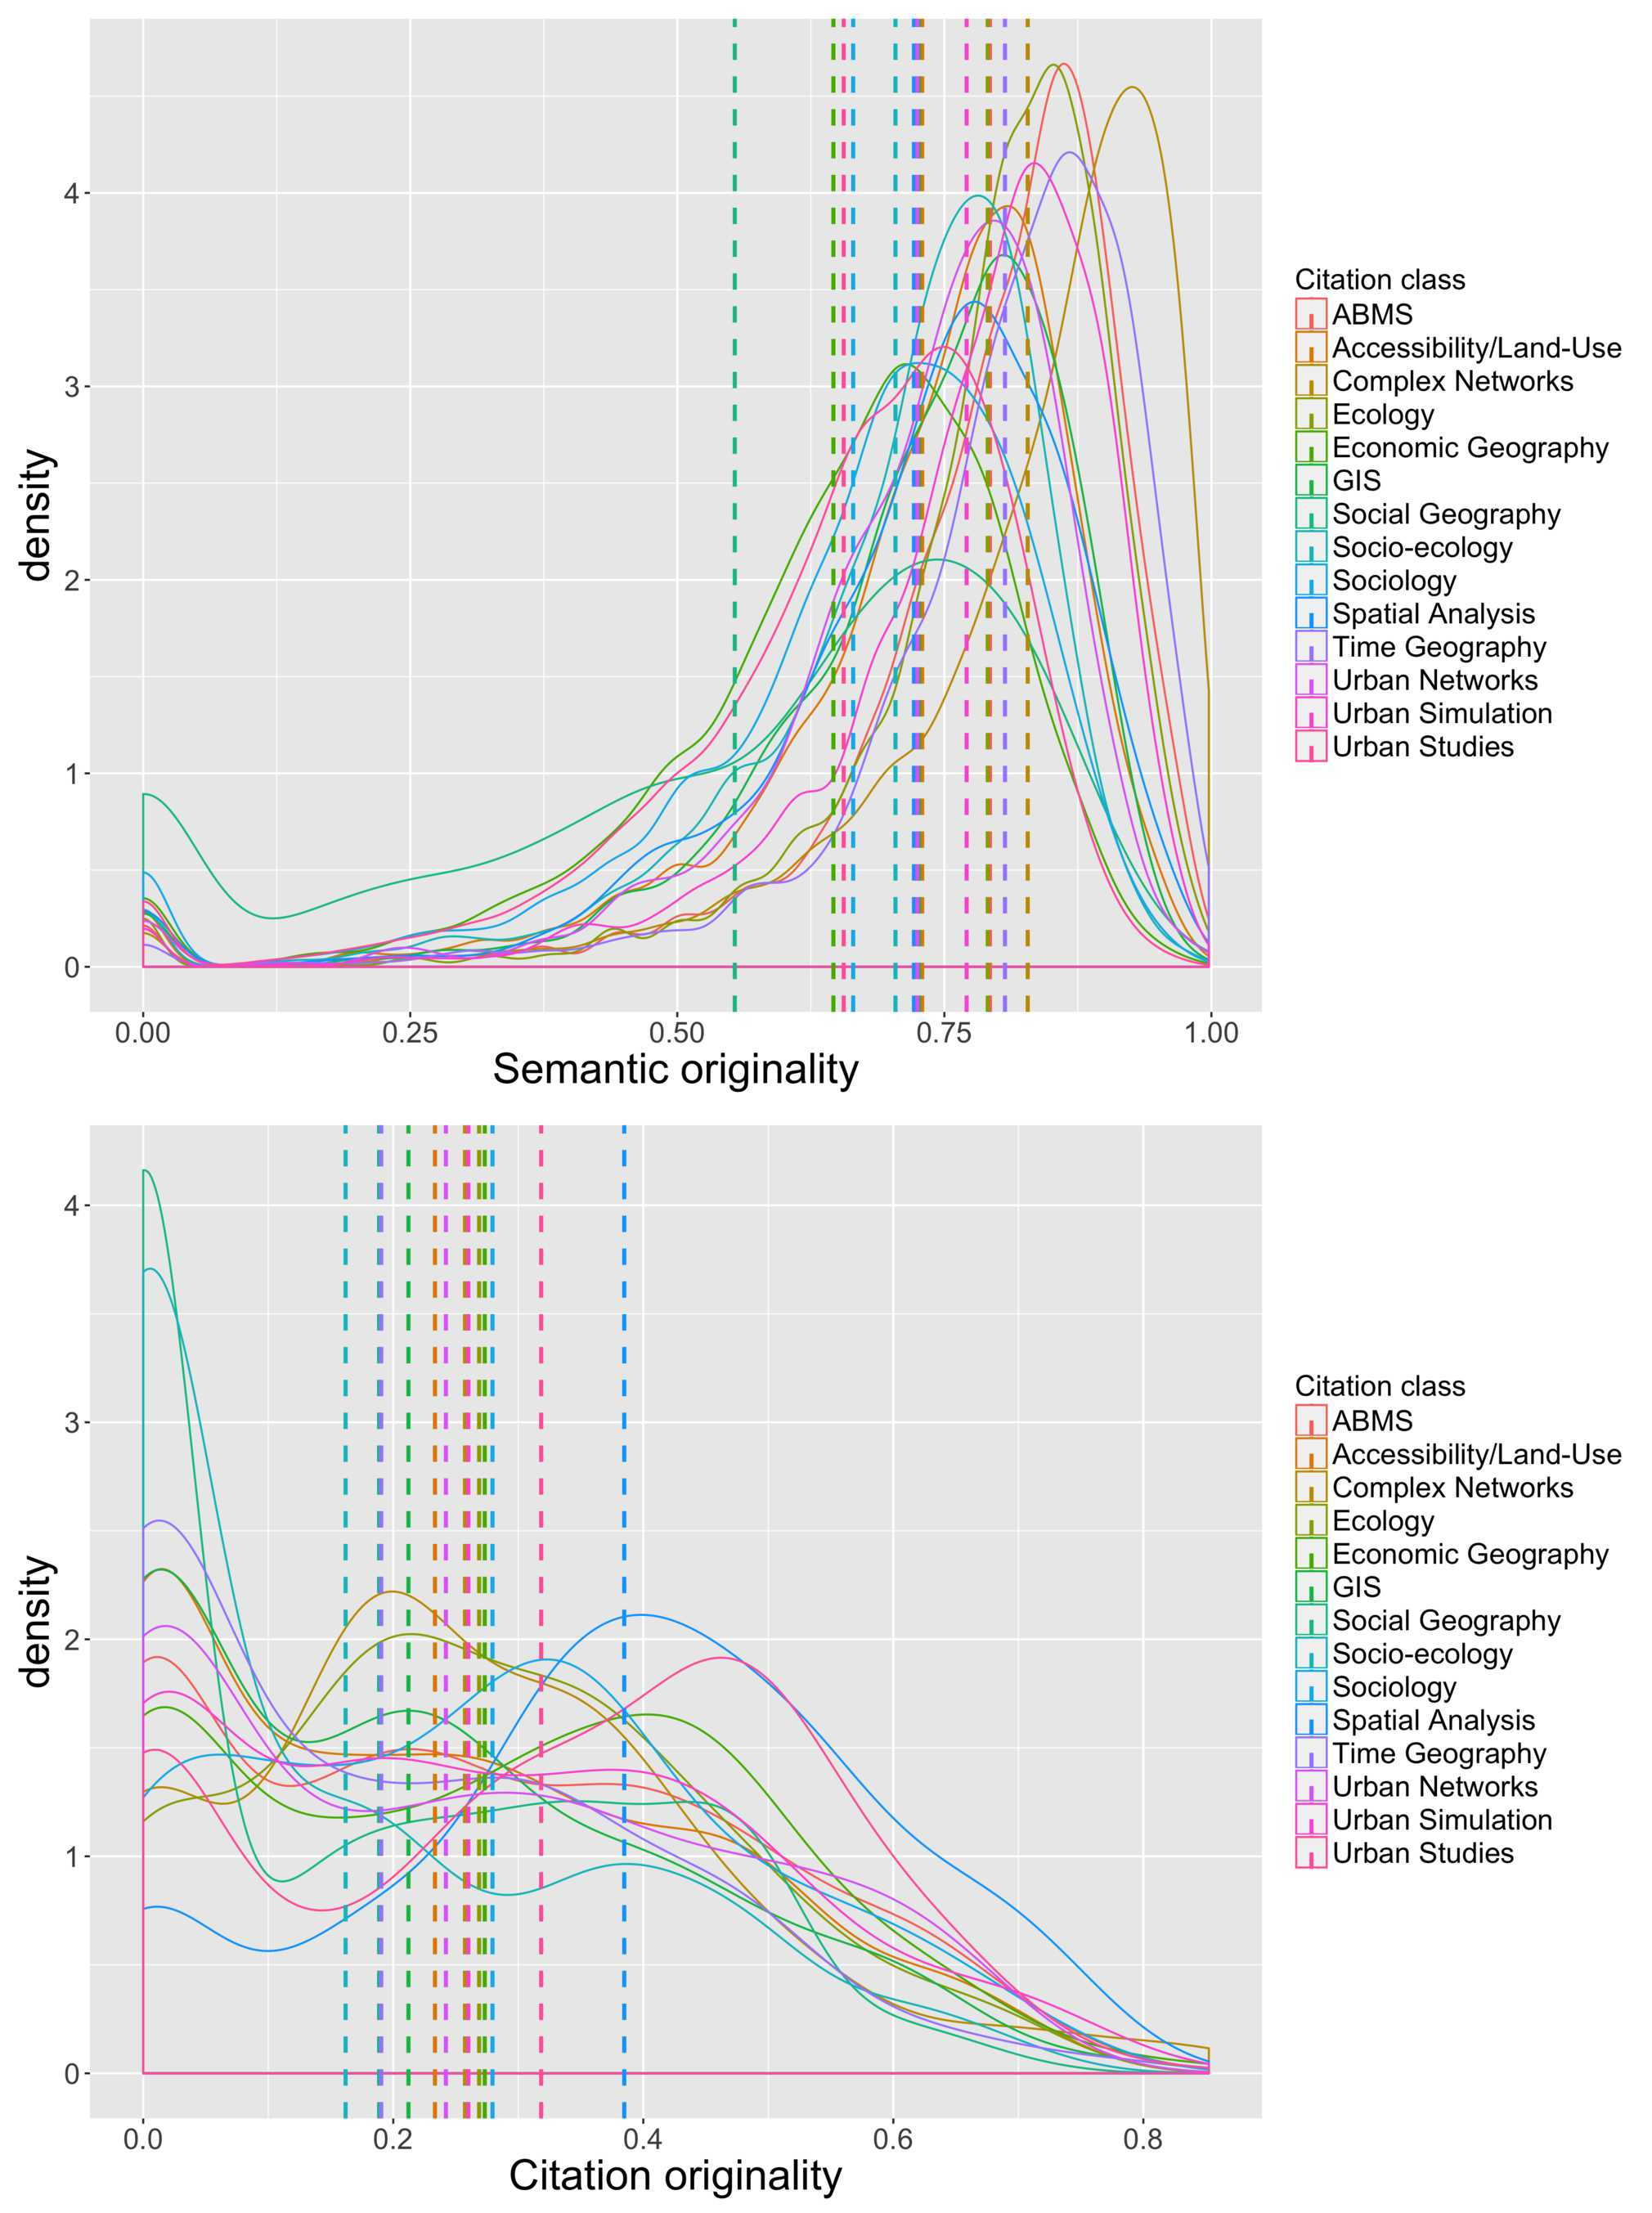
\includegraphics[width=\textwidth]{Figures/Cybergeo/Fig10}
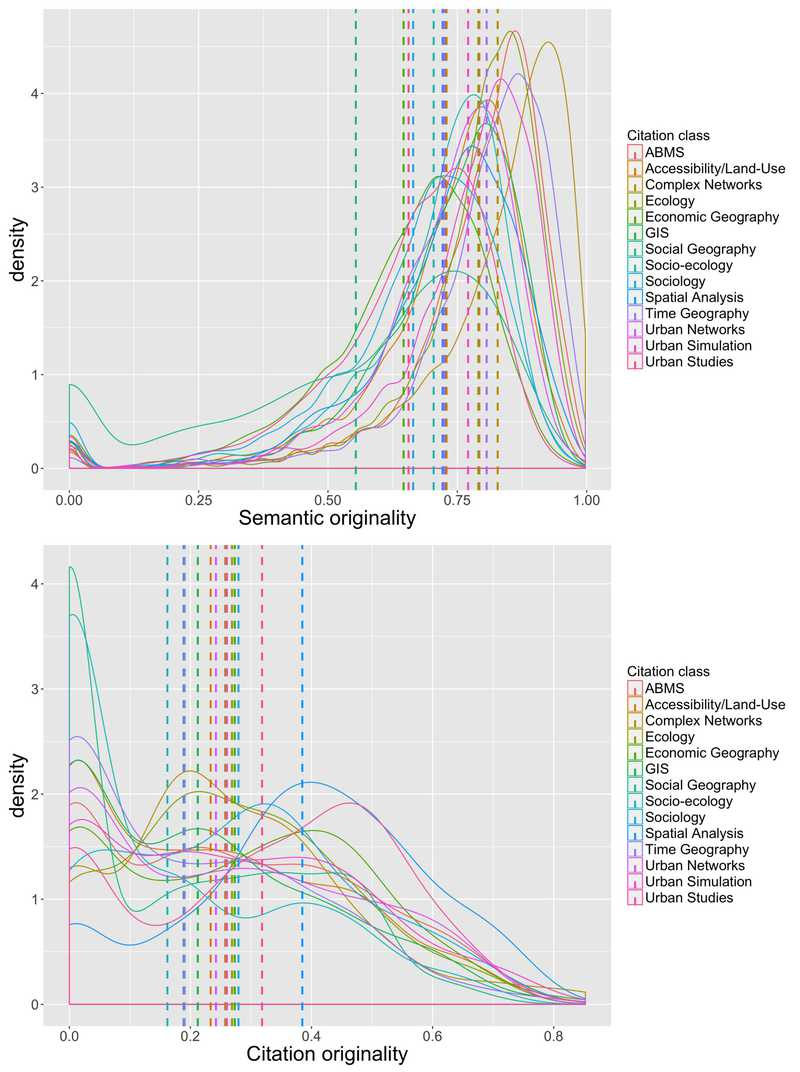
\includegraphics[width=\linewidth,height=0.9\textheight]{Figures/Final/B-cybergeo-fig10.jpg}
\appcaption{\textbf{Statistical distribution of originalities.} We show the smoothed probability densities of originality indexes, by citation class (given by color), for the Semantic originality $o^{(Semantic)}$ (top plot) and for the Citation originality $o^{(Citation)}$ (bottom plot). Dashed lines give the mean for each distribution, with the corresponding color.\label{fig:cybergeo:fig10}}{\textbf{Distribution statistique des originalités.} Nous donnons les densités de probabilité lissées des indices d'originalité, par classe de citation (donnée par la couleur), pour l'originalité sémantique $o^{(Semantic)}$ (\textit{Haut}) et pour l'originalité de citation $o^{(Citation)}$ (\textit{Bas}). Les lignes pointillées donnent la moyenne pour chaque distribution, avec la couleur correspondante.\label{fig:cybergeo:fig10}}
\end{figure}
%%%%%%%%%%%%%%%%%%


\bpar{
We had up to now a qualitative view on interdisciplinarity patterns, by looking at the relative localisation of communities within the citation and semantic classifications, and the relation between the classifications. We propose now to look at quantitative measures of interdisciplinarity, for each classification.
}{
Nous avons eu jusqu'à présent une vue qualitative sur les motifs d'interdisciplinarité, en s'intéressant à la localisation relative des communautés au sein des classifications de citation et sémantique, et la relation entre les classifications. Nous proposons à présent de regarder des mesures quantitatives de l'interdisciplinarité, pour chaque classification.
}

\bpar{
More precisely, for a given classification $C \in \{ Citation,Semantic\}$ a reference $i$ can be viewed as a probability vector $(p_{ij}^{(C)})_j$ on classes $j$ that give for each class the probability to belong to it. Given this setting, we measure interdisciplinarity of one reference using Herfindhal concentration index~\citep{porter2009science}, that can also be called an originality index. We define originality as
}{
Plus précisément, pour une classification donnée $C \in \{ Citation,Semantic\}$ une référence $i$ peut être représentée par un vecteur de probabilités $(p_{ij}^{(C)})_j$ sur les classes $j$ qui donne pour chaque classe la probabilité d'y appartenir. Etant donné cette configuration, nous mesurons l'interdisciplinarité d'une référence en utilisant une concentration d'Herfindhal~\cite{porter2009science}, qui peut aussi être appelée indice d'originalité. Nous définissons l'originalité par
}
\[
o_i^{(C)} = 1 - \sum_j {p_{ij}^{(C)}}^2
\]
\bpar{
For the semantic classification, probabilities are defined as the proportion of keywords of the abstract within each semantic class. With the deterministic citation classification, each reference has only one class and the originality index is always 0. Therefore in order to be able to compare the two classification, we associate a probability to each citation class for each article as the proportion of citations received from this class. The induced index is original, and measures interdisciplinarity as \emph{how a reference is used} by different disciplines in its lifetime.
}{
Pour la classification sémantique, les probabilités sont définies comme la proportion de mots-clés du résumé dans chaque classe sémantique. Avec la classification de citation déterministe, chaque référence a une classe unique et l'index d'originalité est toujours nul. Pour cette raison, afin de pouvoir comparer les deux classifications, nous associons une probabilité à chaque classe de citation pour chaque article comme la proportion de citations reçues de cette classe. L'indice induit est original, et mesure l'interdisciplinarité comme la façon dont une référence \emph{est utilisée} par différentes disciplines pendant sa vie.
}


\bpar{
We show in Fig.~\ref{fig:cybergeo:fig10} the statistical distribution for both indexes $o^{(Semantic)}$ and $o^{(Citation)}$, stratified by citation class. This allow a direct comparison between the two and also an indirect comparison by the variation of semantic distribution between citation classes. For the distribution of semantic originalities, all citation classes exhibit a similar pattern, that is a peak around large values and a smaller peak at zero. It means that either references are highly specialized and have keywords in one class only, or they use keywords from different classes in a quite even manner (for comparison, an abstract with half keywords in a class and half in an other gives an originality of 0.5). The most original, i.e. the most mixed, citation class, is Complex Networks, with a distribution clearly detached from others, what would confirm their use as a method with a lot of different problems. Social Geography is from far the less original, with a large number of single class references, and an average far lower than other classes, what would mean an increased presence of compartmentalization within the associated disciplines.
}{
Nous montrons en Fig.~\ref{fig:cybergeo:fig10} la distribution statistique des deux indices $o^{(Semantic)}$ et $o^{(Citation)}$, stratifiées par classe de citation. Cela permet une comparaison directe entre les deux et également une comparaison indirecte par la variation des distributions sémantiques selon les classes de citations. Pour la distribution des originalités sémantiques, l'ensemble des classes de citation présentent un motif similaire, qui correspond à un pic autour d'une grande valeur et un pic plus faible à zéro. Cela signifie que soit les références sont fortement spécialisées et n'ont des mots-clés que dans une seule classe, ou bien elles utilisent des mots-clés de différentes classes de façon relativement équilibrée (pour comparaison, un résumé avec moitié de mots dans une classe et moitié dans une autre donne une originalité de 0.5). La classe de citation la plus originale, i.e. la plus mélangée, est \textit{Complex Networks}, avec une distribution clairement détachée des autres, ce qui confirmerait leur utilisation comme une méthode pour un certain nombre de problèmes différents. La Géographie sociale est de très loin la moins originale, avec un grand nombre de références à classe unique, et une moyenne bien plus basse que celle des autres classes, ce qui signifierait une présence accrue d'isolation dans les disciplines associées.
}


\bpar{
In terms of citation originality index, the global picture is fundamentally different, as average originality indexes are all lower than 0.4 and most of distributions show their mode in 0, meaning that most references are only cited by their own citation class. Again, Social Geography is the less original, confirming a similar behavior in terms of citation practice than in terms of research content. The most original classes in average, with a peak in large values, are Spatial Analysis and Urban Simulation: this corresponds to the fact that these class feature quite generic methods that can be applied in several fields and are cited accordingly. Complex Networks do not reach the same level, but however exhibit a peak around 0.2 and no peak in 0, together with Ecology, suggesting disciplines having still significant impact in other disciplines.
}{
En termes d'indice d'originalité de citation, le comportement général est fondamentalement différent, les indices d'originalité moyens étant tous inférieurs à 0.4 et la plupart des distributions ont leur mode en 0, ce qui signifie que la majorité des références sont citées uniquement par leur propre classe de citation. A nouveau, la Géographie sociale est la moins originale, confirmant un comportement similaire en termes de pratiques de citation qu'en termes de contenu de la recherche. Les classes les plus originales en moyenne, avec un pic dans les grandes valeurs, sont \textit{Spatial Analysis} et \textit{Urban Simulation} : cela correspond au fait que ces classes contiennent des méthodes relativement génériques qui peuvent être appliquées dans différents champs et sont citées de manière appropriée. Les \textit{Complex Networks} n'atteignent pas le même niveau, mais présentent cependant un pic autour de 0.2 et pas de pic en 0, de la même manière que l'écologie, suggérant des disciplines ayant toujours un impact significatif sur les autres disciplines.
}

\bpar{
To summarize, we show (i) different patterns of interdisciplinarity, depending on disciplines, in terms of scientific content (semantic) and of scientific impact (citation); and (ii) a strong qualitative difference in behavior of originalities between the two classifications, what suggests their complementarity.
}{
En résumé, nous montrons (i) différents motifs d'interdisciplinarité, selon les disciplines, en termes de contenu scientifique (sémantique) et d'impact scientifique (citation) ; et (ii) une forte différence qualitative de comportement des originalités entre les deux classifications, ce qui suggère leur complémentarité.
}


%%%%%%%%%%%%%%%%%%
\subsubsection{Correlation between classifications}{Corrélation entre classifications}

\bpar{
In order to strengthen the idea of a complementarity of classifications, that would each capture different dimensions of processes of knowledge production, we finally look at the correlation matrix between classifications. We use this time effective class probabilities for the citation classification, i.e. a vector of zeros except with a one at the index of the class of the reference. We compute a Pearson correlation coefficient between classes $k$ (in semantic) and $k'$ (in citation) as
}{
Afin de renforcer l'idée d'une complémentarité des classifications, qui captureraient chacune différentes dimensions des processus de production de connaissance, nous examinons finalement la matrice des corrélations entre les classifications. Nous utilisons cette fois les probabilités de classes effectives pour la classification de citation, i.e. un vecteur de zeros à l'exception d'un un à l'index de la classe de la référence. Nous calculons un coefficient de corrélation de Pearson entre les classes $k$ (sémantique) et la classe $k'$ (citation) comme
}
\[
\rho_{k,k'} = \frac{Cov \left[ (p^{(Sem)}_{ik})_i , (p^{(Cit)}_{ik'})_i \right]}{\sqrt{\Var\left[(p^{(Sem)}_{ik})_i\right]\Var\left[(p^{(Sem)}_{ik})_i\right]}}
\]

\bpar{
\noindent where the covariance is estimated with the unbiased estimator.
}{
\noindent où la covariance est estimée avec l'estimateur non biaisé.
}

\bpar{
The structure of the correlation matrix recalls the conclusions obtained when studying the semantic composition of citation communities, such as GIS being strongly correlated with GIS ($\rho=0.26$), or Sociology with Political Science ($\rho=0.16$). More importantly for our question are summary statistics of the overall matrix. It has a minimum of $-0.16$ (Ecology (citation) against Political Sciences (semantic)), an average of $-0.002$ and a maximum of $0.33$ (Social geography (citation) and Spatial Analysis (semantic)). The ``high'' values are highly skewed, as the first decile is at $-0.06$ and the last at $0.09$, what means that 80\% of coefficient lie within that interval, corresponding to low correlations. In a nutshell, classifications are consistent as highest correlations are observed where one can expect them, but most of classes are uncorrelated, meaning that the classifications are quite orthogonal and therefore complementary.
}{
La structure de la matrice de correlation rejoint les conclusions obtenues lors de l'étude de la composition sémantique des communautés de citation, comme le GIS étant fortement corrélé au GIS ($\rho=0.26$), ou la Sociologie à la Science politique ($\rho=0.16$). Plus importantes pour notre questions sont les statistiques de synthèse de la matrice entière. Elle a un minimum de $-0.16$ (\textit{Ecology} (citation) contre les sciences politiques (sémantique)), une moyenne de $-0.002$ et un maximum de $0.33$ (\textit{Social geography} (citation) et \textit{Spatial Analysis} (sémantique)). Les valeurs ``fortes'' sont fortement isolées, comme le premier décile est à $-0.06$ et le dernier à $0.09$, ce qui signifie que 80\% des coefficients tombent dans cet intervalle, correspondant à des corrélations faibles. En résumé, les classifications sont cohérentes puisque les corrélations les plus fortes sont observées où on peut les attendre, mais la majorité des classes ne sont pas corrélées, ce qui signifie que les classifications sont relativement orthogonales et ainsi complémentaires.
}



%summary(as.numeric(rho))
%      Min.    1st Qu.     Median       Mean    3rd Qu.       Max. 
%-0.1631820 -0.0397953 -0.0187894 -0.0003216  0.0089678  0.3262073 

%summary(as.numeric(rho[,2:ncol(rho)]))
%     Min.   1st Qu.    Median      Mean   3rd Qu.      Max. 
% -0.157525 -0.039676 -0.018789 -0.001669  0.008007  0.326207 


% correlation matrix between classifications

%                                                NA Complex Networks      Ecology Social Geography
%health                                 0.084217277      0.015642565 -0.031280002    -0.0304122878
%crime                                 -0.034264269     -0.027466263 -0.030184851    -0.0109058566
%statistical methods                   -0.045196471     -0.009985336  0.134773697    -0.0427562039
%remote sensing                         0.008677423     -0.039616065  0.004274342    -0.0001037131
%political sciences/critical geography -0.163182024     -0.063553835 -0.157524519     0.0103925609
%traffic modeling                       0.135493504     -0.025760072 -0.053805346    -0.0401532076
%microbiology                           0.005013388      0.069833747  0.175721643    -0.0428300111
%cognitive sciences                    -0.057904751      0.021390559 -0.008878000    -0.0183249948
%spatial analysis                      -0.028954136     -0.040284497  0.038681879     0.3262073464
%GIS                                   -0.068226509     -0.025851971 -0.027627123    -0.0355896609
%biogeography                           0.157670367     -0.065793131  0.155044018    -0.0622661875
%environnment/climate                   0.146864511     -0.016857698  0.081698376    -0.0499190937
%economic geography                    -0.036386086     -0.088454740 -0.131327817    -0.0516875579
%physical geography                     0.155877876     -0.050479420  0.044855501    -0.0342161549
%                                         Sociology          GIS Spatial Analysis         ABMS Socio-ecology
%health                                -0.035281096 -0.027390702    -0.0092406664 -0.028471411  -0.039977735
%crime                                 -0.003511700 -0.016330983    -0.0034925253 -0.026372584  -0.016182744
%statistical methods                    0.006204335  0.009875529     0.0006603197  0.016162014  -0.048901119
%remote sensing                        -0.022526140 -0.008140740     0.0161506994  0.051559757   0.009078915
%political sciences/critical geography  0.164538990  0.070441824    -0.0099431496 -0.070547880   0.092456547
%traffic modeling                       0.006759964  0.003892643    -0.0200454337  0.004937954   0.009572245
%microbiology                          -0.010887689 -0.004926871    -0.0256598780  0.032859898  -0.025374219
%cognitive sciences                     0.189133684  0.021302626    -0.0233197884 -0.012683768  -0.039854983
%spatial analysis                      -0.039550918 -0.026571766    -0.0200352507 -0.019253896  -0.036900317
%GIS                                   -0.044445811  0.266230113    -0.0196994093  0.008379501  -0.048098115
%biogeography                          -0.090286092 -0.047362187    -0.0314376536  0.118217762   0.063732285
%environnment/climate                  -0.061530547 -0.043172212    -0.0228268820 -0.010868666   0.042866717
%economic geography                    -0.007205760 -0.080607481     0.1107474038 -0.087310233  -0.080743040
%physical geography                    -0.077603719 -0.024403758    -0.0309332281 -0.007944706   0.177918682
%                                      Urban Networks Urban Simulation Urban Studies Economic Geography
%health                                   0.227985960      0.003101104  -0.011951445       -0.029092421
%crime                                   -0.007323995      0.151779291   0.037625633        0.007882492
%statistical methods                      0.002304641      0.074944283  -0.047068353       -0.019986633
%remote sensing                           0.011034168     -0.007373975   0.009064606       -0.008777581
%political sciences/critical geography    0.024982340     -0.129188848   0.250087262        0.123687818
%traffic modeling                        -0.026107672     -0.016873541  -0.020788824       -0.056640509
%microbiology                            -0.031639788     -0.015875901  -0.048817564       -0.039139437
%cognitive sciences                      -0.024141333      0.006168384  -0.017845169       -0.051689224
%spatial analysis                        -0.022931057      0.004936436  -0.048686678       -0.027250467
%GIS                                     -0.031369284      0.107217335  -0.059539768       -0.055057115
%biogeography                            -0.038744405     -0.019857075  -0.093015237       -0.081157234
%environnment/climate                    -0.003931271     -0.009427780  -0.061113194       -0.052661932
%economic geography                       0.035747109      0.070533726   0.036039127        0.154483917
%physical geography                      -0.013960728     -0.003533876  -0.058702622       -0.064289131
%                                      Accessibility/Land-Use Time Geography
%health                                          -0.020422023   -0.026027683
%crime                                           -0.009526164   -0.019419266
%statistical methods                             -0.008130459   -0.008458811
%remote sensing                                  -0.009152899   -0.023371493
%political sciences/critical geography           -0.073794569   -0.017737603
%traffic modeling                                 0.035398096   -0.020400327
%microbiology                                    -0.055066210   -0.003858738
%cognitive sciences                              -0.049222763    0.141081799
%spatial analysis                                 0.007710532   -0.009041103
%GIS                                             -0.033615280    0.237580646
%biogeography                                    -0.029578349   -0.062363162
%environnment/climate                             0.012457860   -0.055488257
%economic geography                               0.213283602   -0.087410630
%physical geography                              -0.069686740   -0.037465822
%








%%%%%%%%%%%%%%%%%%
\subsection{Discussion}{Discussion}
%%%%%%%%%%%%%%%%%%


\bpar{
We have this way shown the complementarity of classifications in the qualitative patterns they unveil, but also quantitatively in terms of interdisciplinarity measures and quantitatively in terms of correlations. Our work can be extended regarding several aspects, of which we give some suggestions below.
}{
Nous avons ainsi montré la complémentarité des classifications dans les motifs qualitatifs qu'elles dévoilent, mais aussi quantitativement en termes de mesures d'interdisciplinarité et quantitativement en termes de corrélations. Notre travail peut être étendu selon différents aspects, desquels nous donnons certaines suggestions par la suite.
}

\subsubsection{Further Developments}{Développements}


\bpar{
A first development consists in the comparison of journals. The starting point for construction of the scientific environment, the journal \textit{Cybergeo}, was the entry point but not the subject of our study. A development more focused on journals, trying for example to answer comparative issues, or to classify journals according to their effective level of interdisciplinarity regarding different dimensions, would be potentially interesting. The collection of precise data on the origin of references is however a first step that need to be solved first.
}{
Un premier développement consiste en la comparaison de journaux. Le point de départ pour la construction de l'environnement scientifique, le journal \textit{Cybergeo}, était le point d'entrée mais pas le sujet principal de notre étude. Un développement se concentrant plus sur les journaux, essayant par exemple de répondre à des questions comparatives, ou de classifier les journaux selon leur niveau effectif d'interdisciplinarité selon différentes dimensions, serait potentiellement intéressant. La collection de données précises sur l'origine des références est cependant un premier point qui doit d'abord être résolu.
}


\bpar{
The performance of the semantic classification was also not quantified here. A further validation of the relevance of using complementary information contained in both classifications could be done by the analysis of modularities within the citation network, as done in~\cite{bergeaud2017classifying}. This would however require a baseline classification to compare with, which is not available in the type of data we use. Open repository such as arXiv (for physics mainly) or Repec (for Economics) provide API to access metadata including abstracts, and could be starting points for such targeted case studies.
}{
La performance de la classification sémantique n'a également pas été quantifiée ici. Une validation approfondie de la pertinence en utilisant l'information complémentaire contenue dans les deux classifications pourrait être menée par l'analyse des modularités dans le réseau de citation, comme fait dans~\cite{bergeaud2017classifying}. Cela nécessiterait cependant une classification de référence pour comparaison, qui n'est pas disponible avec le type de données que nous utilisons. Des archives ouvertes comme arXiv (principalement pour la physique) ou Repec (pour l'économie) fournissent des API pour accéder aux métadonnées incluant les résumés, et pourraient être des points de départ pour de telles études ciblées.
}



\subsubsection{Applications}{Applications}


\bpar{
A first potential application of our methodology relies on the facts that both classifications unveils thematic domains (objects of study), classical disciplines, methodological communities. These different types of communities can indeed be understood as different \emph{Knowledge Domains}. \cite{raimbault2017applied} postulates co-evolving Knowledge Domains in every process of scientific knowledge production, that are Theoretical, Empirical, Modeling, Methodology, Tools and Data domains. Most of them are necessary for any process, and investigations within one conditions the advances in others. A refinement of classifications, associated with supervised classification to associate knowledge domains to some communities (potentially using full texts to have more precise information on the proportion of each knowledge domains involved in each), would allow to quantify relations between domains. Furthermore, using temporal data with the date of publications, would yield an effective quantification of the \emph{co-evolution} of domains in the sense of patterns of temporal correlations (e.g. Granger causality).
}{
Une première application potentielle de notre méthodologie se base sur le fait que les deux classifications dévoilent à la fois des domaines thématiques (objets d'étude), des disciplines classiques, des communautés méthodologiques. Ces différents types de communautés peuvent en effet être comprises comme différents \emph{Domaines de Connaissance}. \cite{raimbault2017applied} postule des Domaines de Connaissance en co-évolution dans tout processus de production de connaissance scientifique, qui sont les domaines Théorique, Empirique, des Modèles, Méthodologique, des Outils et des Données. La majorité sont nécessaire pour tout processus, et les investigations dans l'un conditionne les avances dans les autres. Un raffinement des classifications, associé à une classification supervisée pour associer des domaines de connaissance à des communautés (en utilisant potentiellement les textes complets pour avoir une information plus précise sur la proportion de chaque domaine de connaissance impliqué dans chaque), permettrait de quantifier les relations entre domaines. De plus, l'utilisation de données temporelles avec les dates des publications, fournirait une quantification effective de la \emph{co-évolution} des domaines au sens des motifs de corrélations temporelles (e.g. causalité de Granger).
}


\bpar{
An other interesting direction is the application of our classifications to the quantification of spatial diffusion of knowledge, as \cite{maisonobe2013diffusion} does for the diffusion of a specific question in genetics. It is not clear if different dimensions of knowledge diffuse the same way: for example citation practices can be correlated to social networks and thus exhibit different patterns than effective research contents. Therefore, our work would allow to study such questions from complementary point of views.
}{
Une autre direction intéressante est l'application de nos classifications à la quantification de la diffusion spatiale de la connaissance, comme \cite{maisonobe2013diffusion} fait pour la diffusion d'un question spécifique en génétique. Il n'est pas évident si des dimensions différentes de la connaissance se diffusent de la même façon : par exemple les pratiques de citation peuvent être corrélées aux réseaux sociaux et peuvent ainsi montrer différents motifs que les contenus effectifs de la recherche. Ainsi, notre travail permettrait d'étudier de telles questions de points de vue complémentaires.
}

\bpar{
Finally, we believe the tool we developed can contribute to an increased empowerment of authors and to the development of open science practices. Among the various visions of Open Science~\citep{fecher2014open}, the opening of data is always an important aspect, together with a development of reflexivity in all disciplines, beyond the sole Social Sciences to which it is classically associated. The first point is dealt with by our open tools for dataset construction, whereas the second is implied by the new knowledge of the different dimensions of the scientific environment we studied.
}{
Enfin, nous affirmons que les outils que nous avons développé peuvent contribuer à une autonomisation accrue des auteurs et au développement de pratiques de science ouverte. Au sein des différentes visions de la Science Ouverte~\cite{fecher2014open}, l'ouverture des données est toujours un aspect important, en même temps d'un développement de la réflexivité dans toutes les disciplines, au delà des seules sciences sociales auxquelles elle est classiquement associée. Le premier point est traité par nos outils ouverts pour la construction de jeux de données, tandis que le second est impliqué par la connaissance nouvelle des différentes dimensions de l'environnement scientifique que nous avons étudié.
}







%%%%%%%%%%%%%%%%%%
\subsection{Conclusion}{Conclusion}
%%%%%%%%%%%%%%%%%%


\bpar{
We have introduced a multi-dimensional approach to the understanding of interdisciplinarity, based on citation network and semantic network analysis. Starting from a generalist journal in Geography, we construct a large corpus of the citation neighborhood, from which we extract relevant keywords to elaborate a semantic classification. We then show qualitatively and quantitatively the complementarity of classifications. The methodology and associated tools are open and can be reused in similar studies for which data is difficult to access or poorly referenced in classical databases.
}{
Nous avons introduit une approche multi-dimensionnelle pour la compréhension de l'interdisciplinarité, basée sur les analyses du réseau de citation et du réseau sémantique. A partir d'un journal généraliste en Géographie, nous construisons un vaste corpus du voisinage de citation, duquel nous extrayons les mots-clés pertinents pour élaborer une classification sémantique. Nous montrons ensuite qualitativement et quantitativement la complémentarité des classifications. La méthodologie et les outils associés sont ouverts et peuvent être réutilisés dans des études similaires pour lesquelles les données sont difficiles à obtenir ou faiblement référencées dans les bases classiques. 
}


\stars


%%%%%%%%%%%%%%%%%%%%%
%%%%%%%%%%%%%%%%%%%%%

%\subsection*{acknowledgements}{Remerciements}
%The author would like to thank the editorial board of Cybergeo, and more particularly Denise Pumain and Christine Kosmopoulos, for having offered the opportunity to work on that subject and provided the production database of the journal. 





